\section{Application Overview}
\label{sec:application_overview}

Having introduced the foundational principles as well as the application and market model architecture in preceding sections, this section provides an overview over the major interfaces that are available in the game. The new implementation can be separated into three major categories of views:

\begin{itemize}
  \item \textbf{Administration Views:} The administrator views can only be accessed with a previously created and authorized user account. New users can be created from the corresponding view in the administrator environment.
  \item \textbf{Team Views:} The team views are only accessible for teams that have been created in a game that is at least in a planned state.
  \item \textbf{Reporting:} The reporting screens are visible to both administrators and teams of a game, as they share the same information. It is planned to differentiate the displayed information based on the role of the user in future extensions. Administrators could e.g. be able to display additional details and team decisions.
\end{itemize}

\subsection{Administration Views}
\subsubsection{Administrator Login}
An administrator needs to have a login to access administrative functionalities. After entering his game master credentials on \Cref{fig:admin_login}, the administrator is authorized and redirected to the game overview.
\begin{figure}[h!]
  \centering
  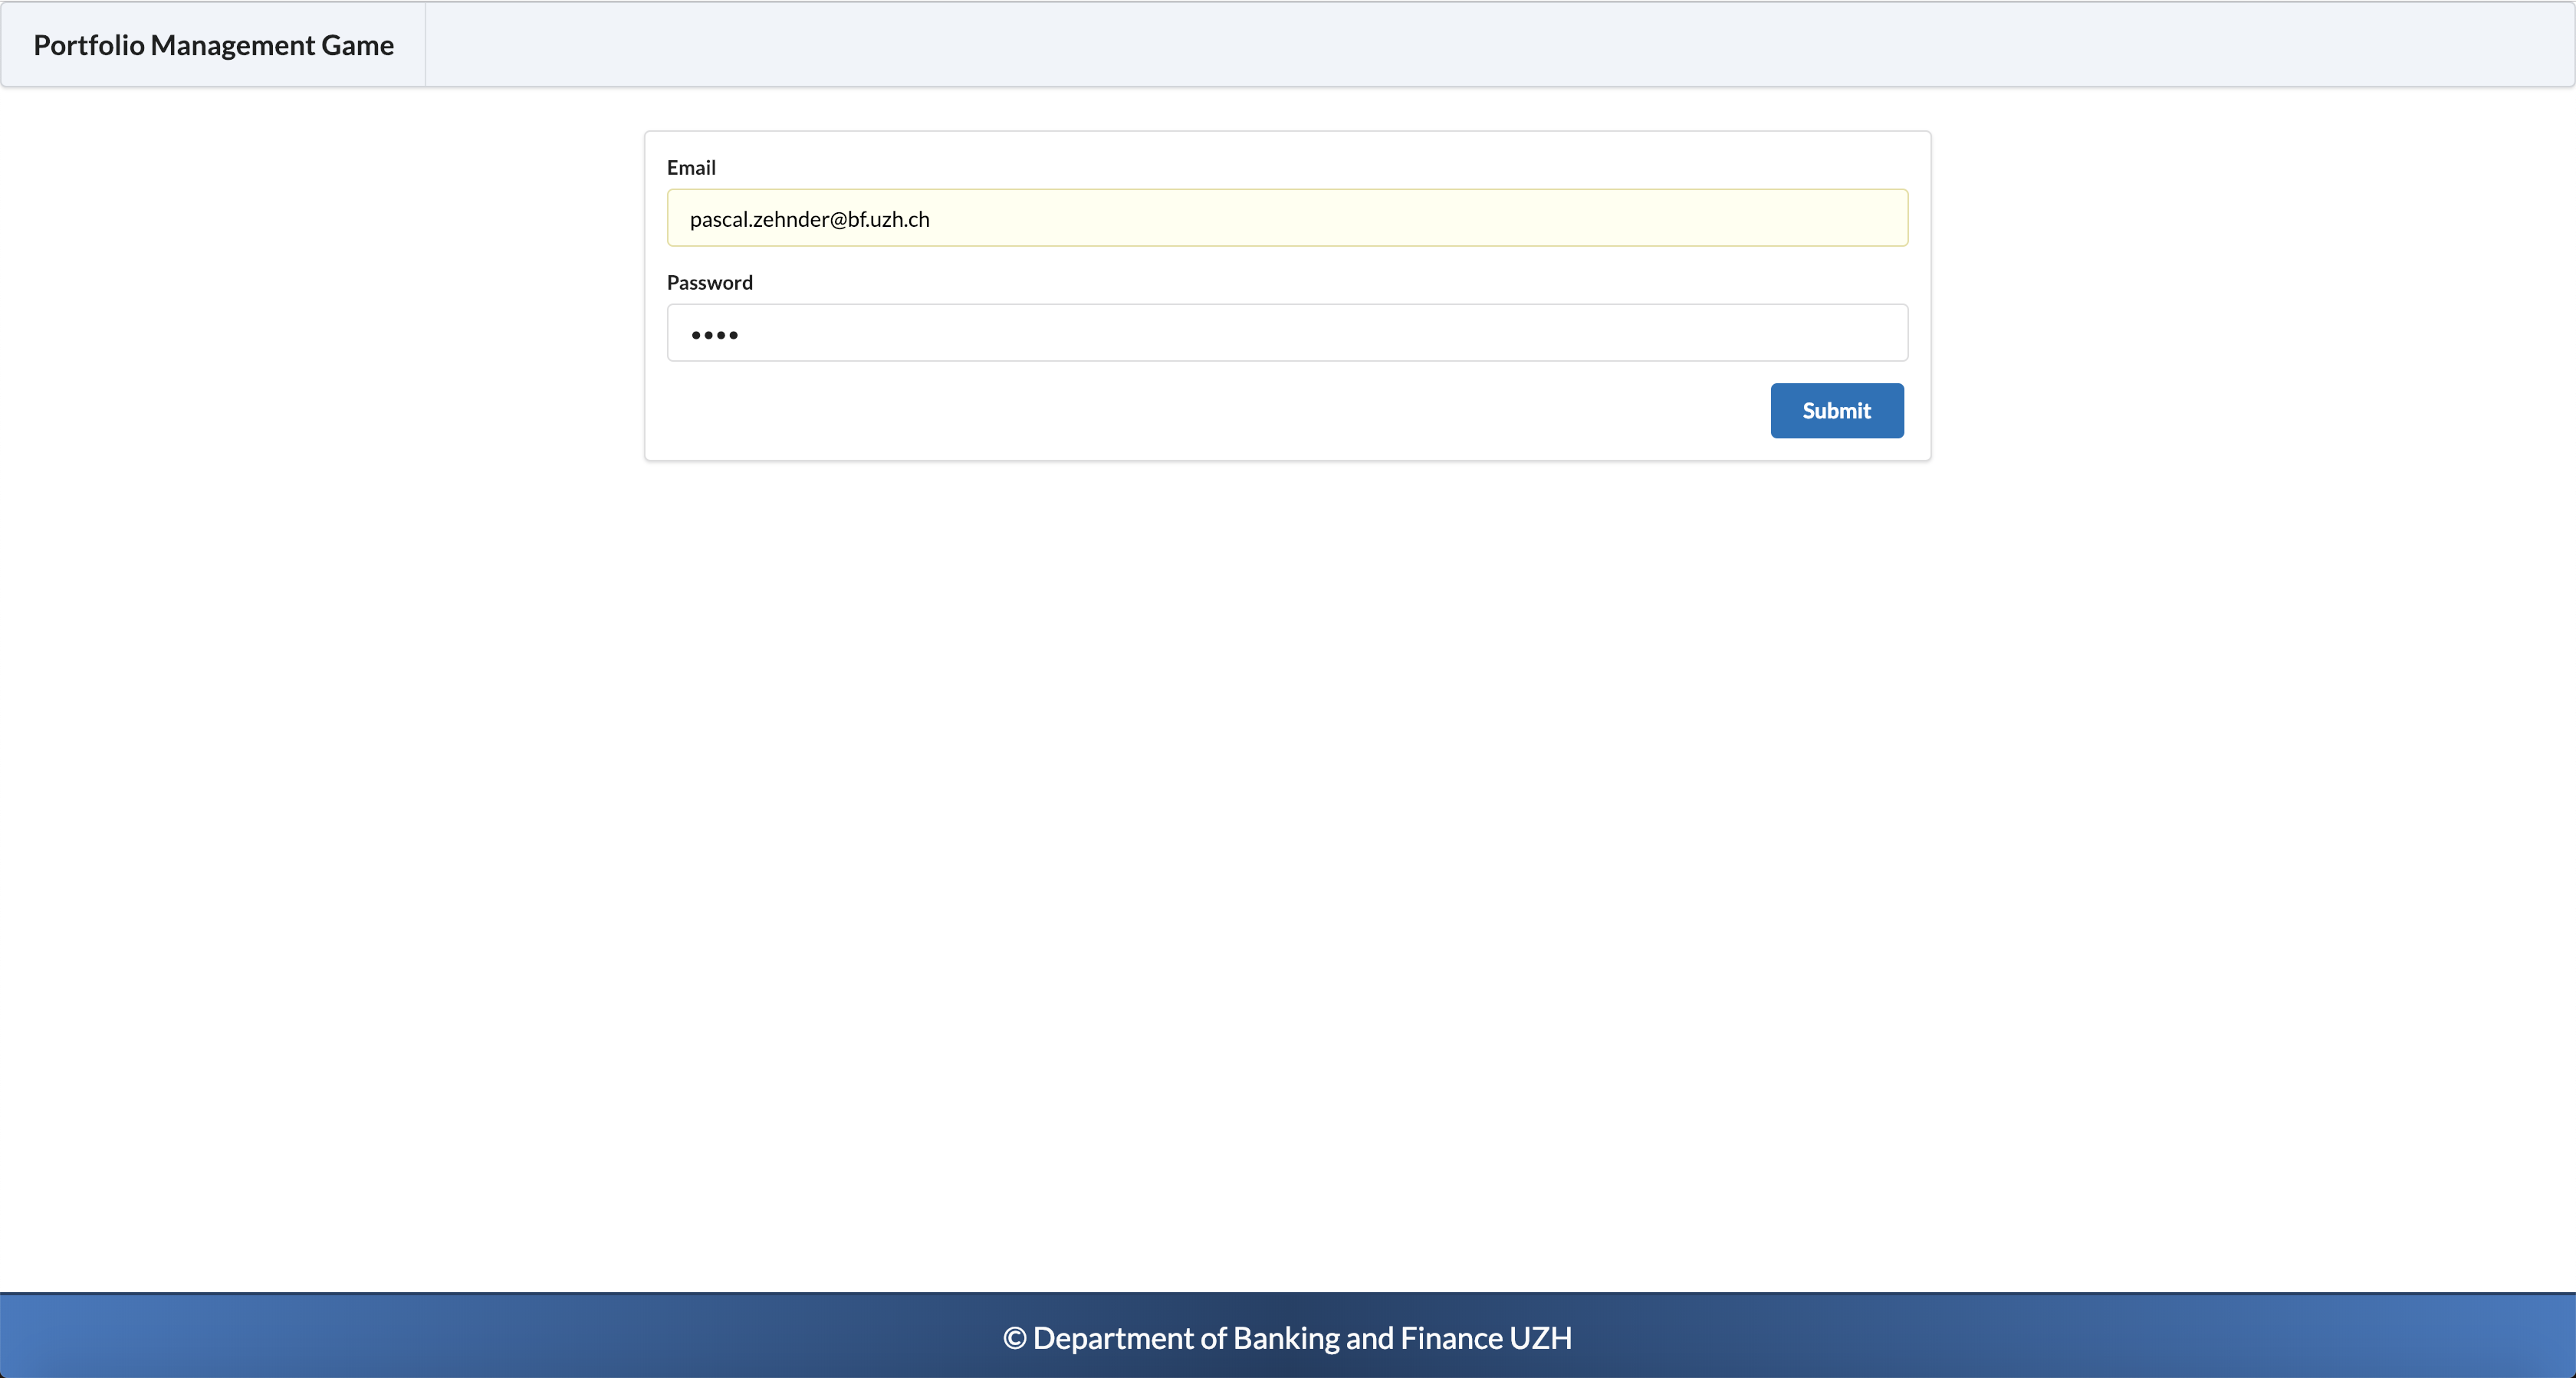
\includegraphics[scale=0.2]{img/application-overview/administrator/01_login.png}
  \caption{Administrator Login}
  \label{fig:admin_login}
\end{figure}

\subsubsection{Game Management}

\paragraph{Game Overview}
The landing page the administrator is redirected to after a successful login is the game overview (\Cref{fig:game_overview}). It serves as a control center, as multiple games can be maintained simultaneously by a single game master. Some instant information identifies the current progress of the game within the list, such as game name, short game id or the current phase of the game.
\begin{figure}[h!]
  \centering
  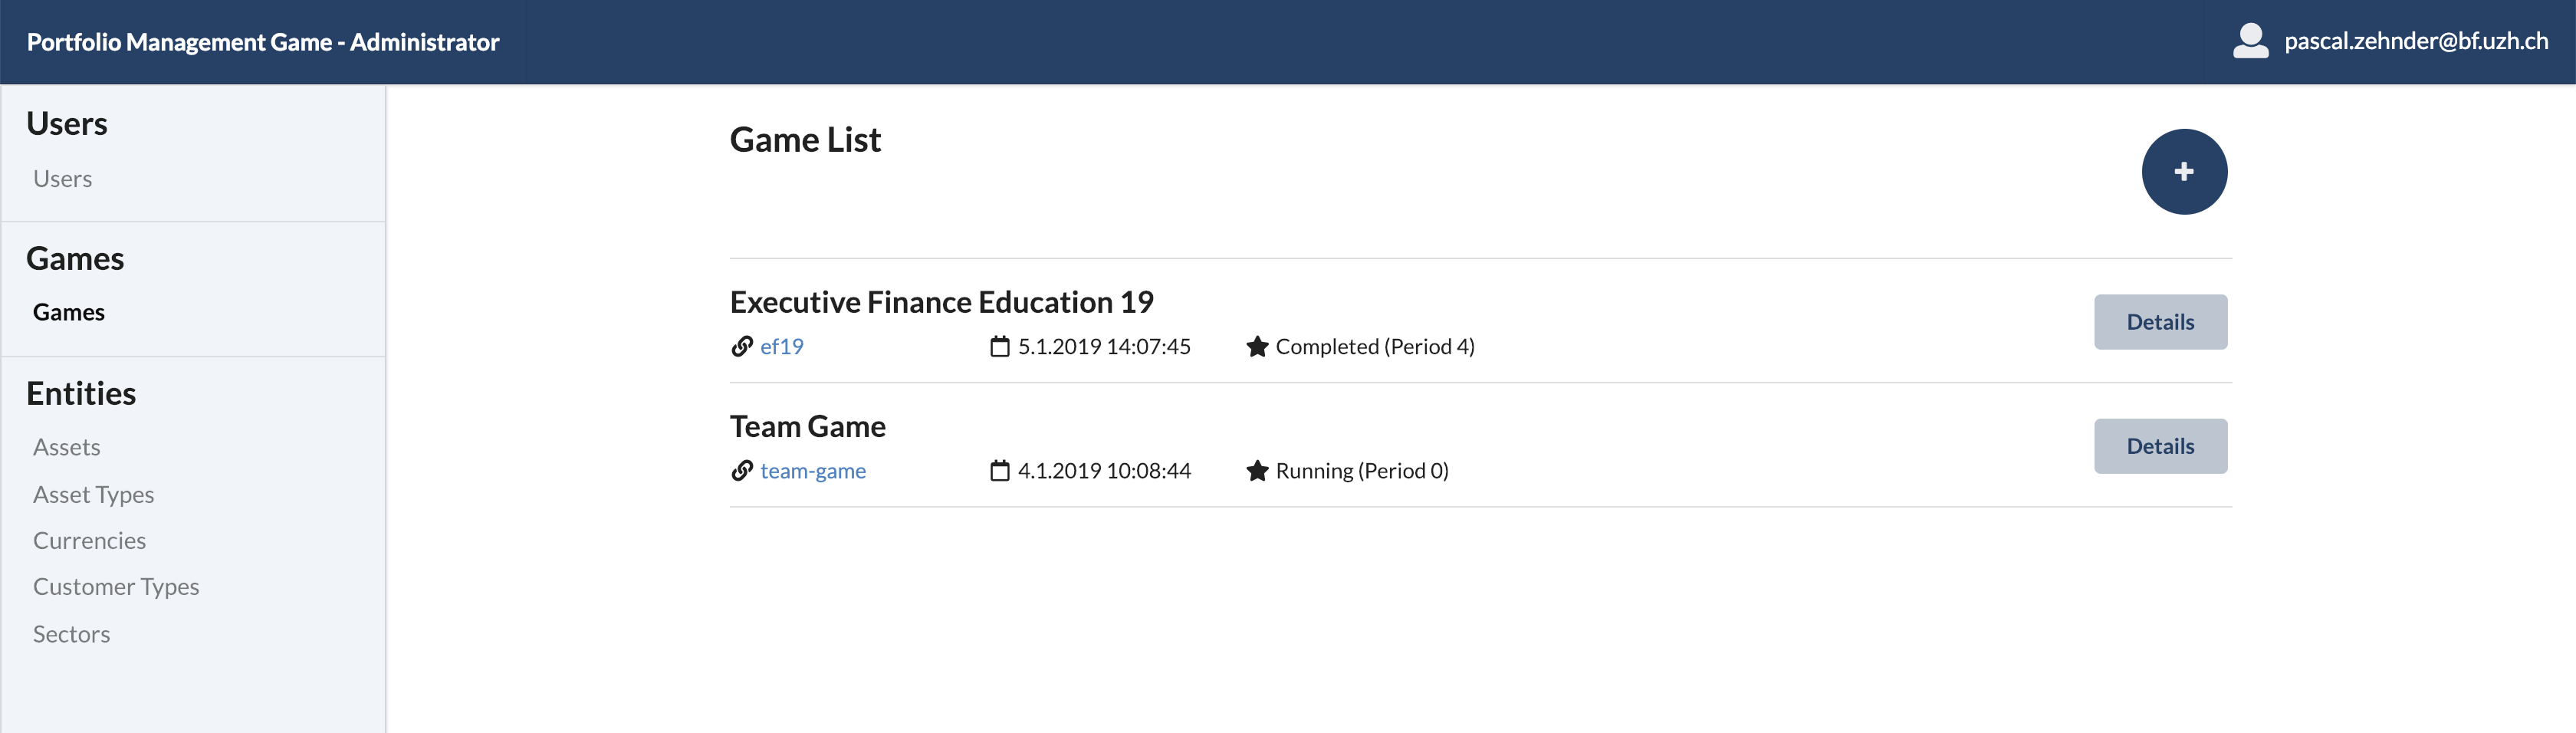
\includegraphics[scale=0.2]{img/application-overview/administrator/02_game_overview.png}
  \caption{Game Overview}
  \label{fig:game_overview}
\end{figure}

\paragraph{Game Creation}
When creating a game the administrator needs to define some parameters by filling out a form (\Cref{fig:game_creation}) structured into three steps. By pressing on the ``next''-button, the administrator will be led through the form. Some tooltips help users to understand the purpose of the input to provide.
\begin{figure}[h!]
  \centering
  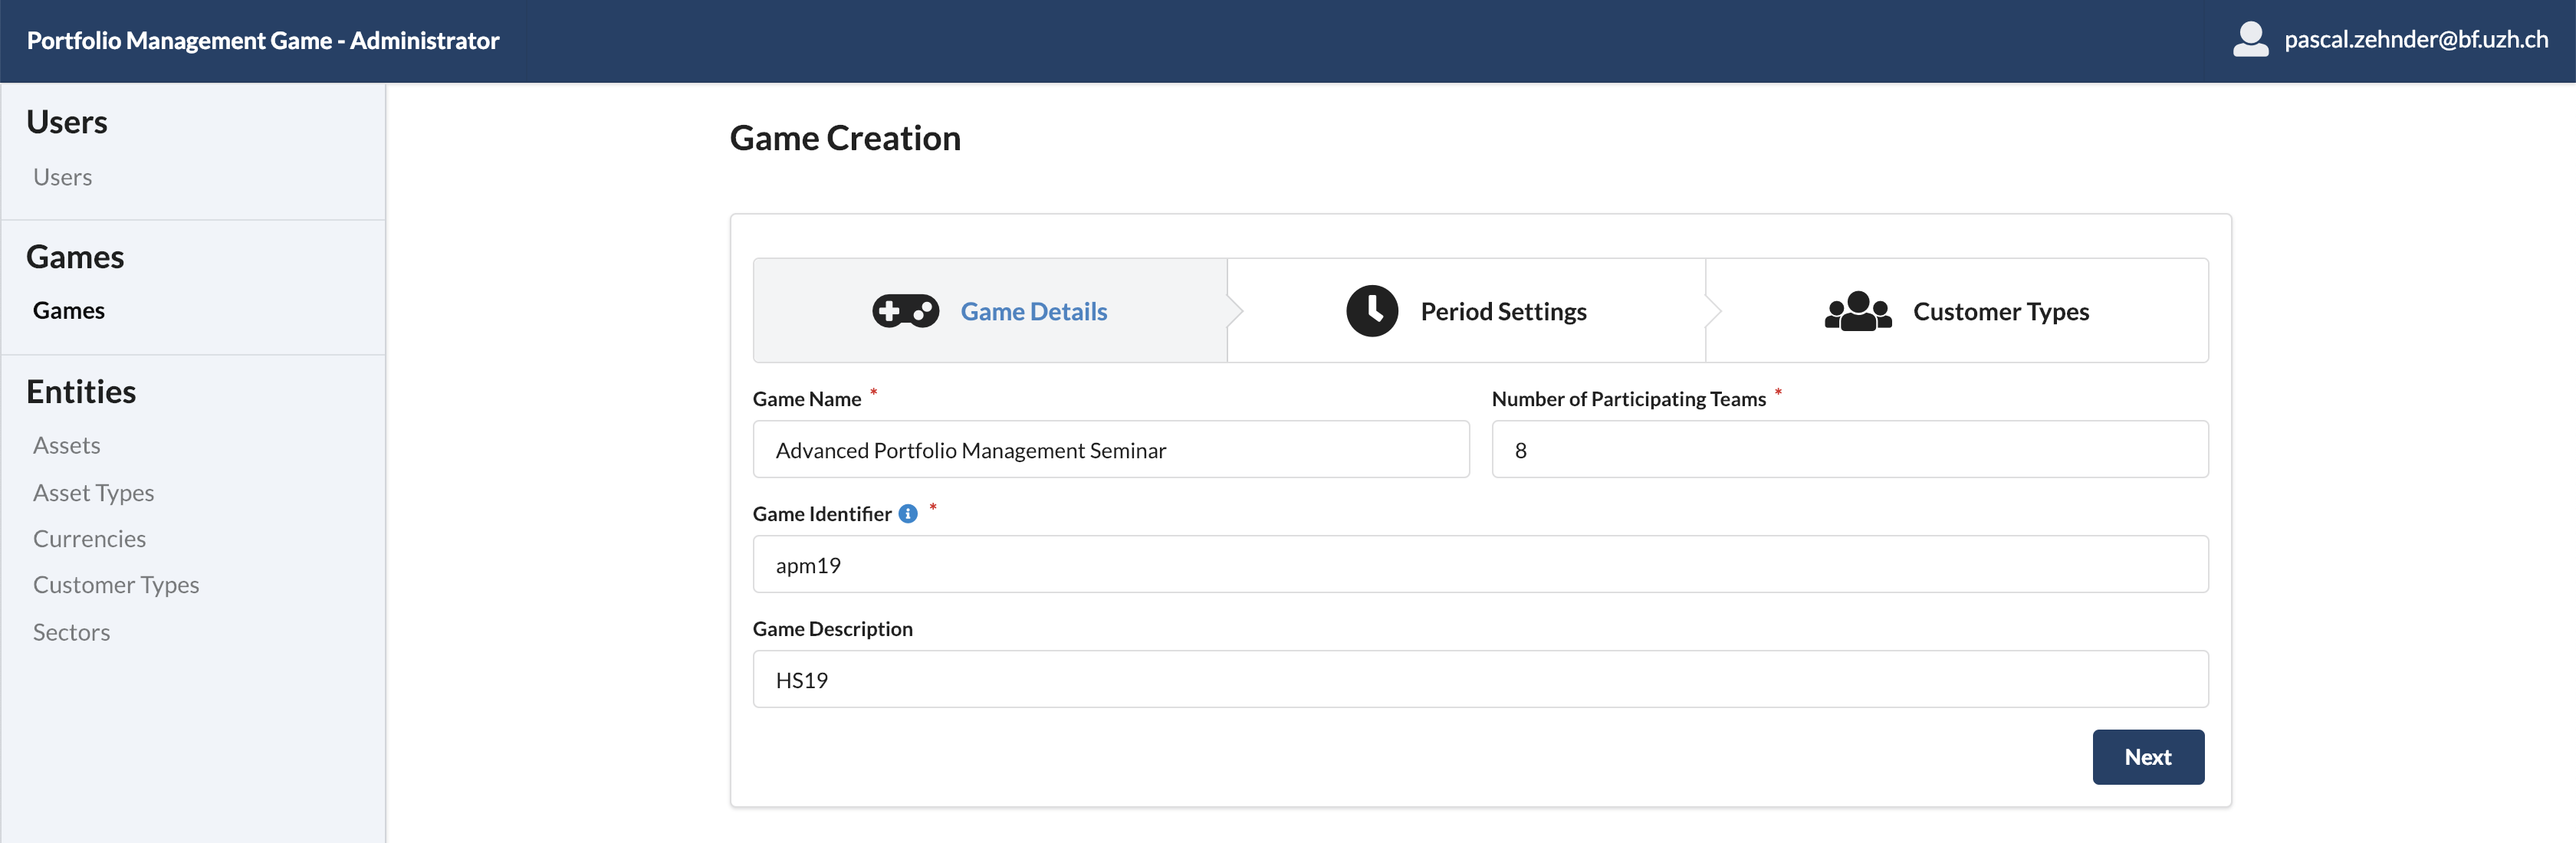
\includegraphics[scale=0.2]{img/application-overview/administrator/03_game_creation.png}
  \caption{Game Creation}
  \label{fig:game_creation}
\end{figure}

\paragraph{Game Initialization}
The game detail for each game may be accessed over the game overview list, as seen in \Cref{fig:game_overview}.  As the game creation may be done in advance we have split the game creation from the game initialization (\Cref{fig:game_initialization}), such that final adjustments of the game may be done just before the start of the game.
\begin{figure}[h!]
  \centering
  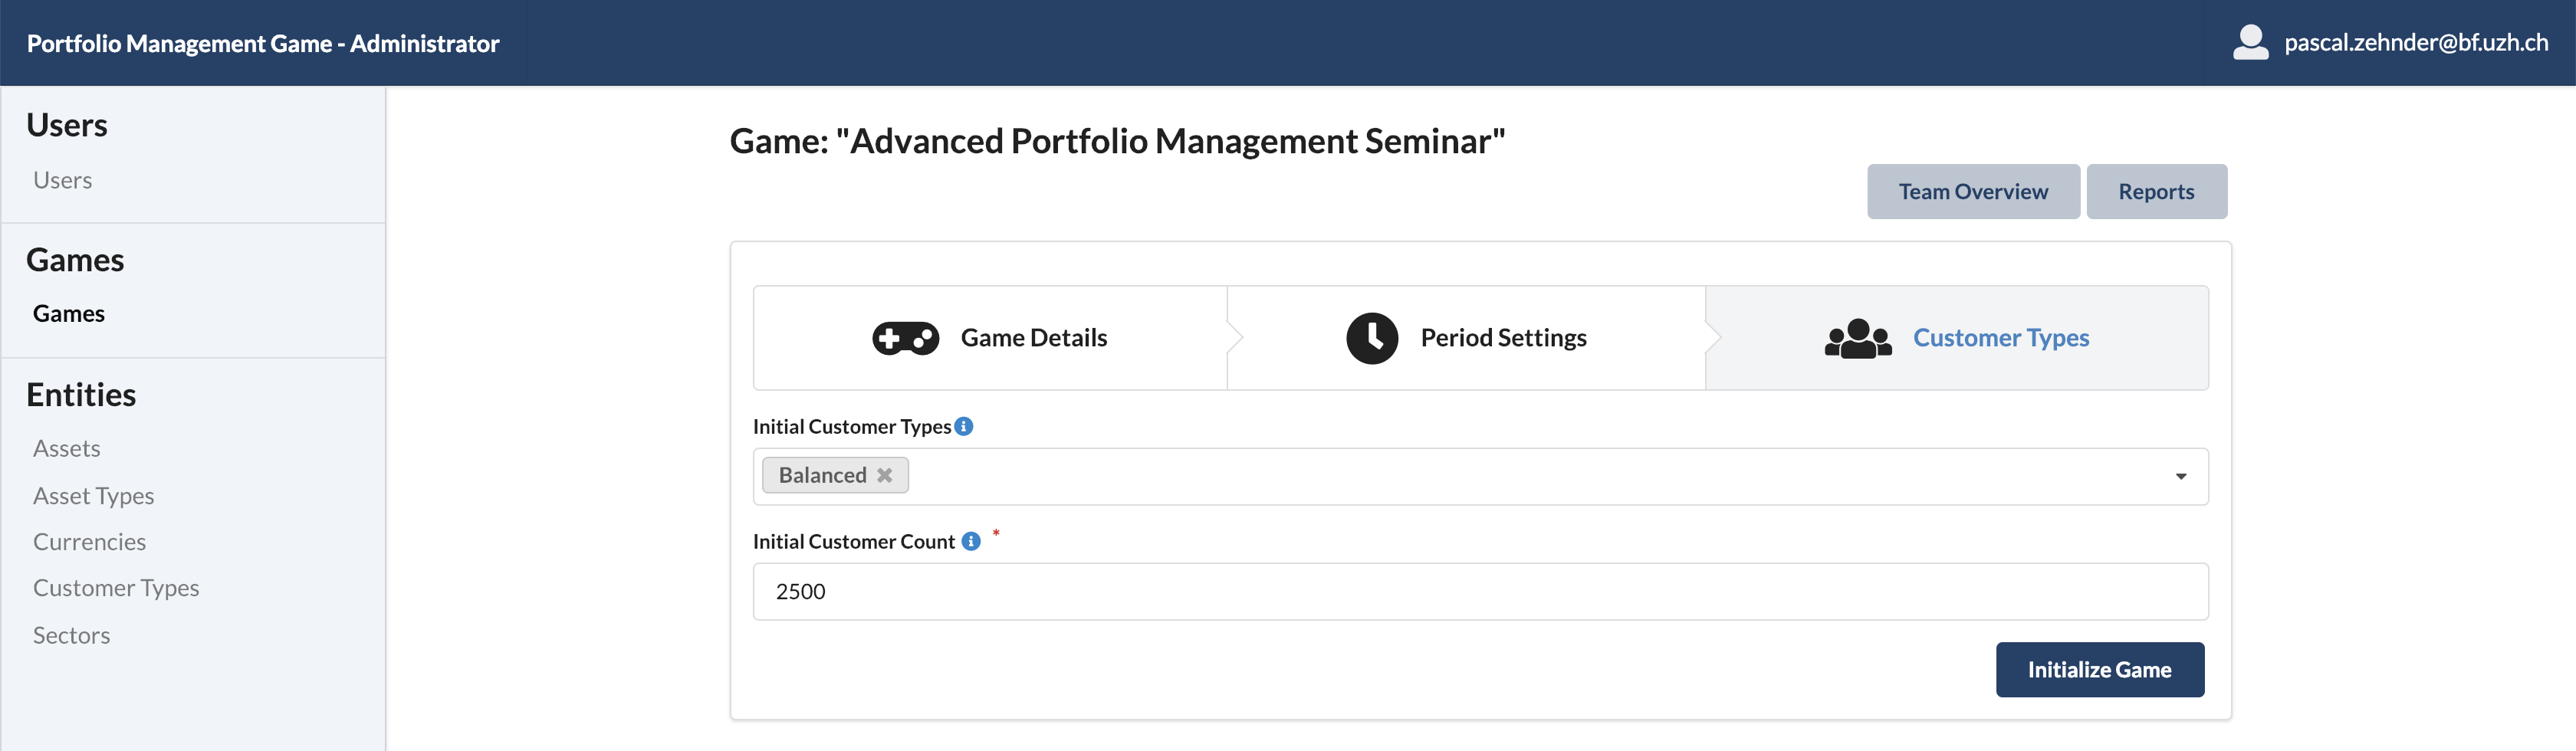
\includegraphics[scale=0.2]{img/application-overview/administrator/04_game_initialization.png}
  \caption{Game Initialization}
  \label{fig:game_initialization}
\end{figure}

\paragraph{Team Overview}
For each team participating in a game, a random password is generated on game creation. To view a list of all team credentials, the administrator can open the team overview as seen on \Cref{fig:team_overview}.
\begin{figure}[h!]
  \centering
  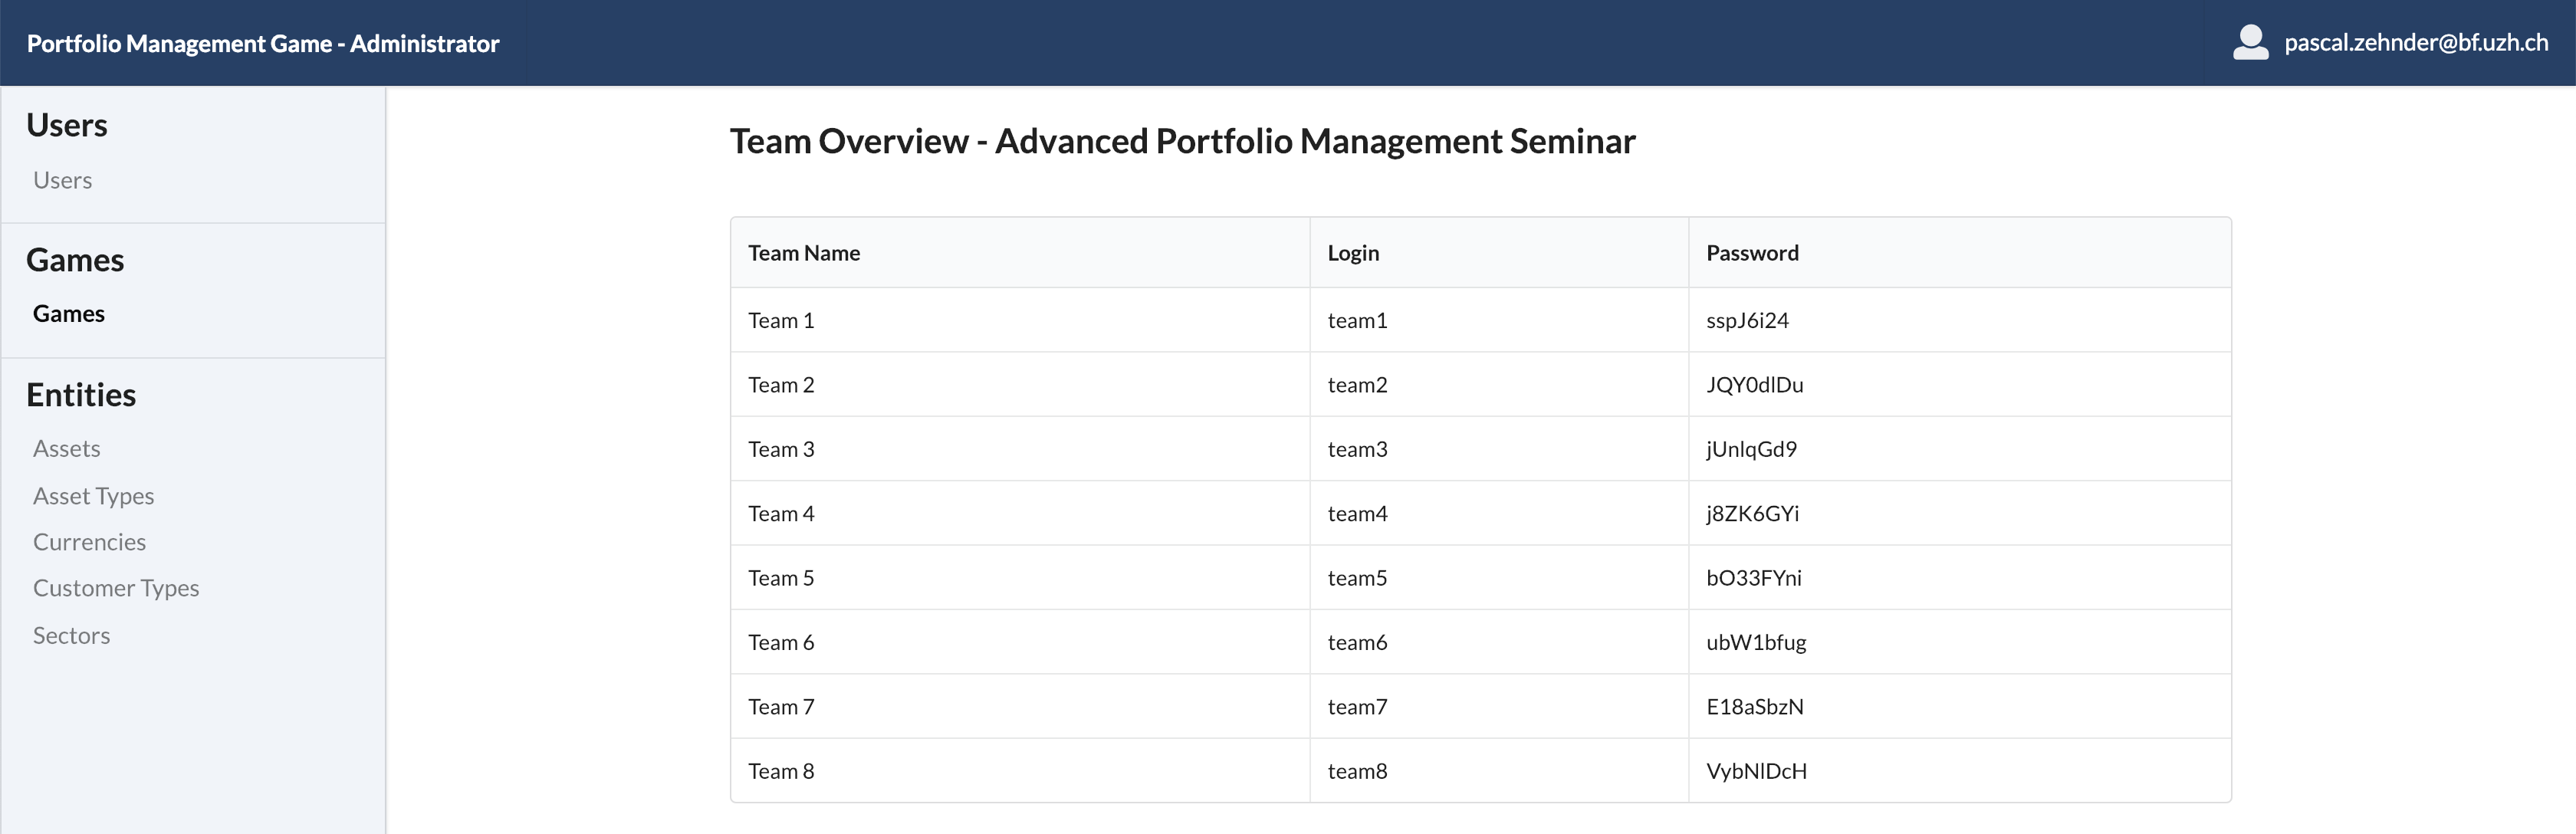
\includegraphics[scale=0.2]{img/application-overview/administrator/06_team_login_overview.png}
  \caption{Team Overview}
  \label{fig:team_overview}
\end{figure}

\paragraph{Game Start}
After starting a game, the students or teams are able to start with their period zero decisions. Administrators are able to give their participants some guidance with messages that will be visible for the teams in their report section. \Cref{fig:game_start} shows a game that is still planned and may be started in a next step.
\begin{figure}[h!]
  \centering
  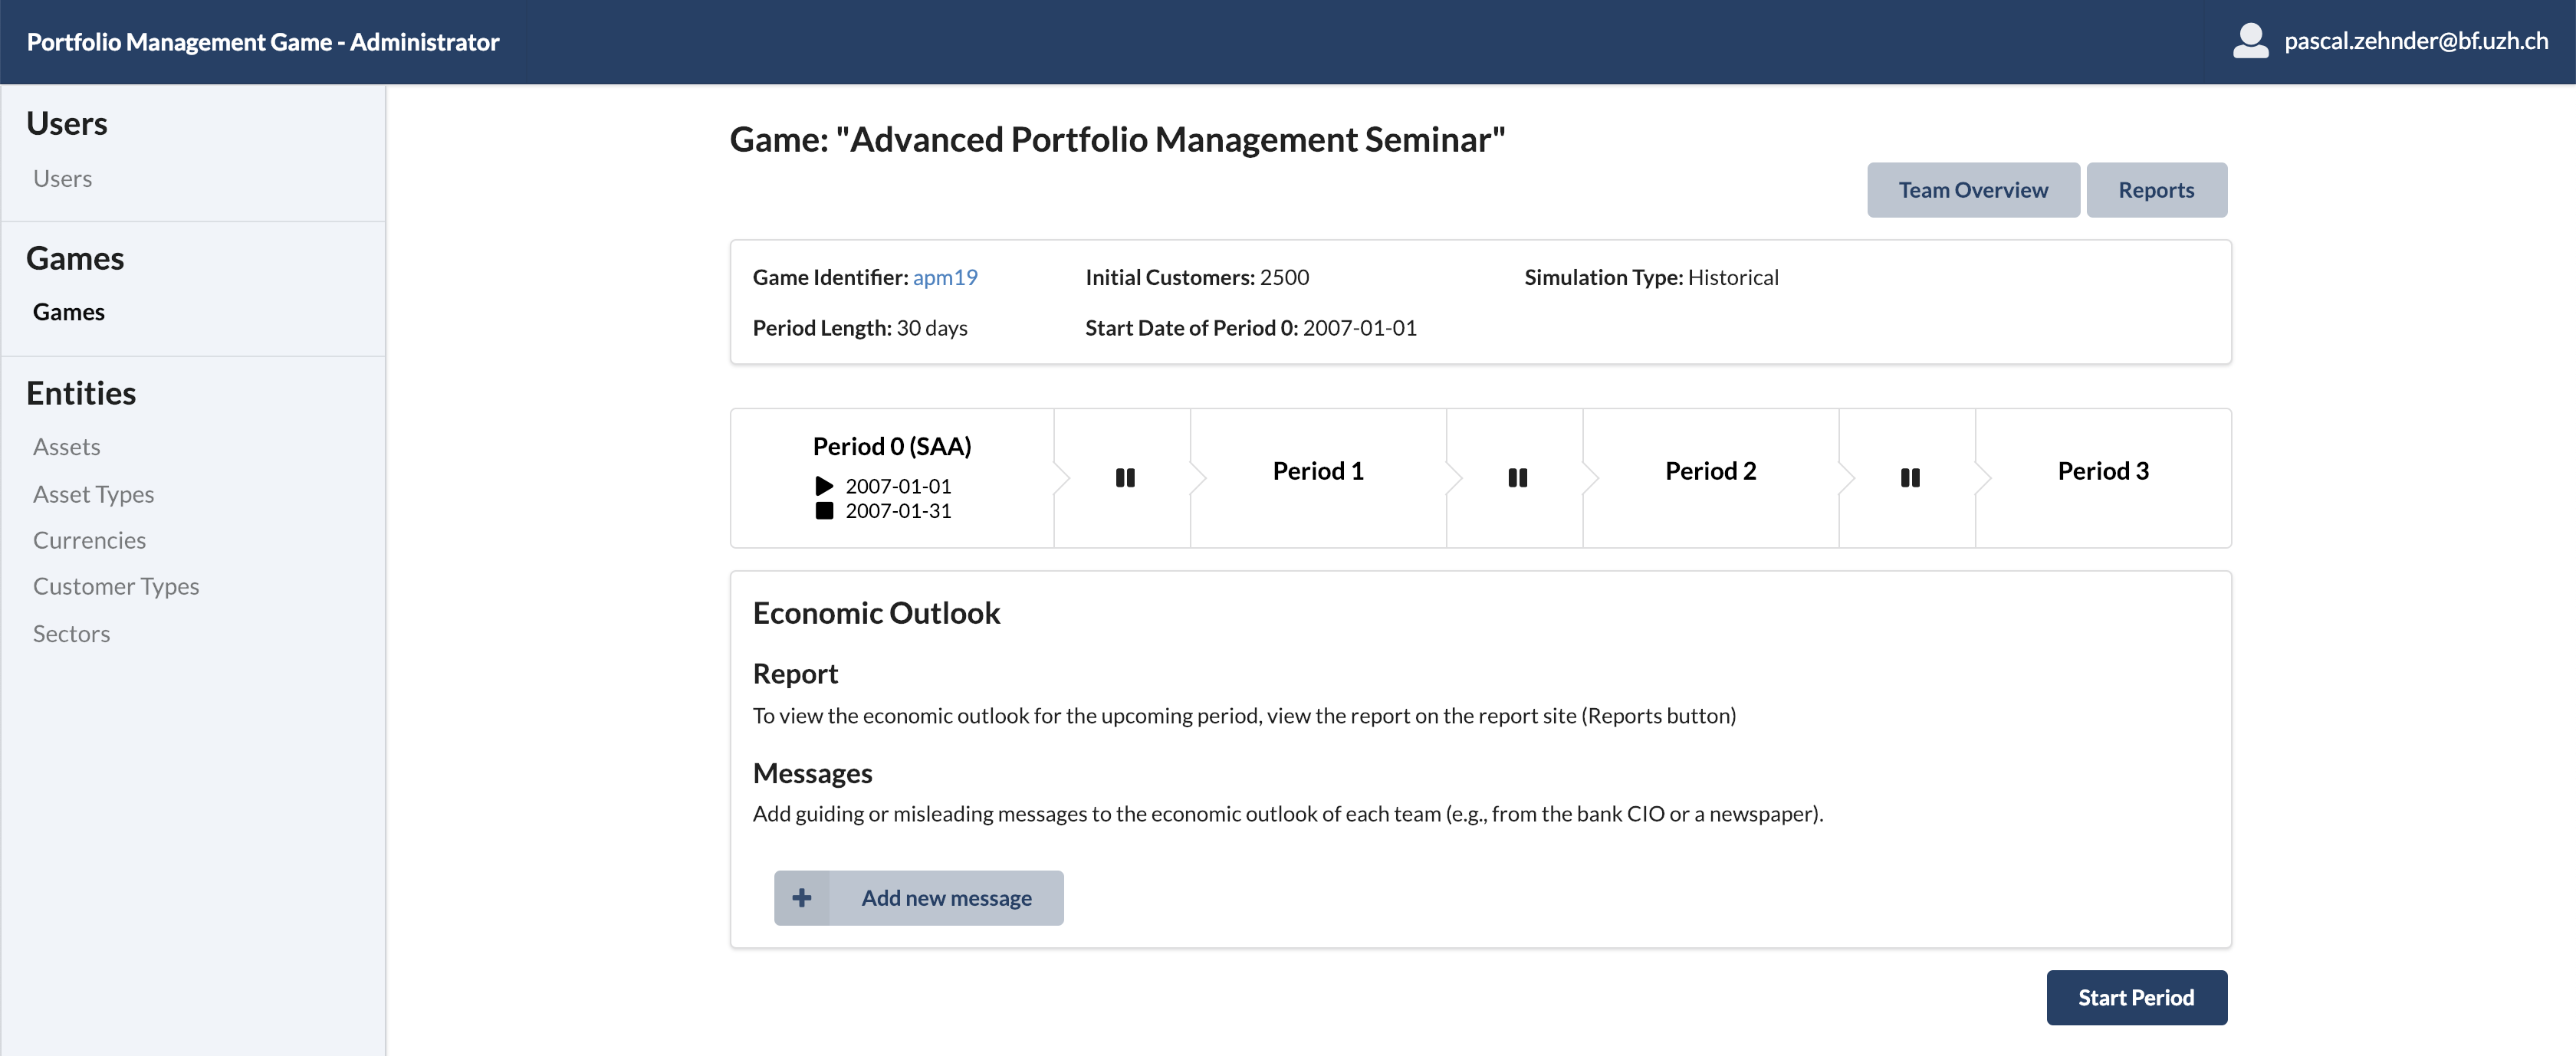
\includegraphics[scale=0.2]{img/application-overview/administrator/05_game_start.png}
  \caption{Game Start}
  \label{fig:game_start}
\end{figure}

\paragraph{Running Period Zero}
When a period is running, the game detail screen shows an overview of the submission state of all teams (\Cref{fig:running_period}). The period can only be finished once all teams have submitted a decision. The administrator is further able to get an insight about the SAA decisions of teams.
\begin{figure}[h!]
  \centering
  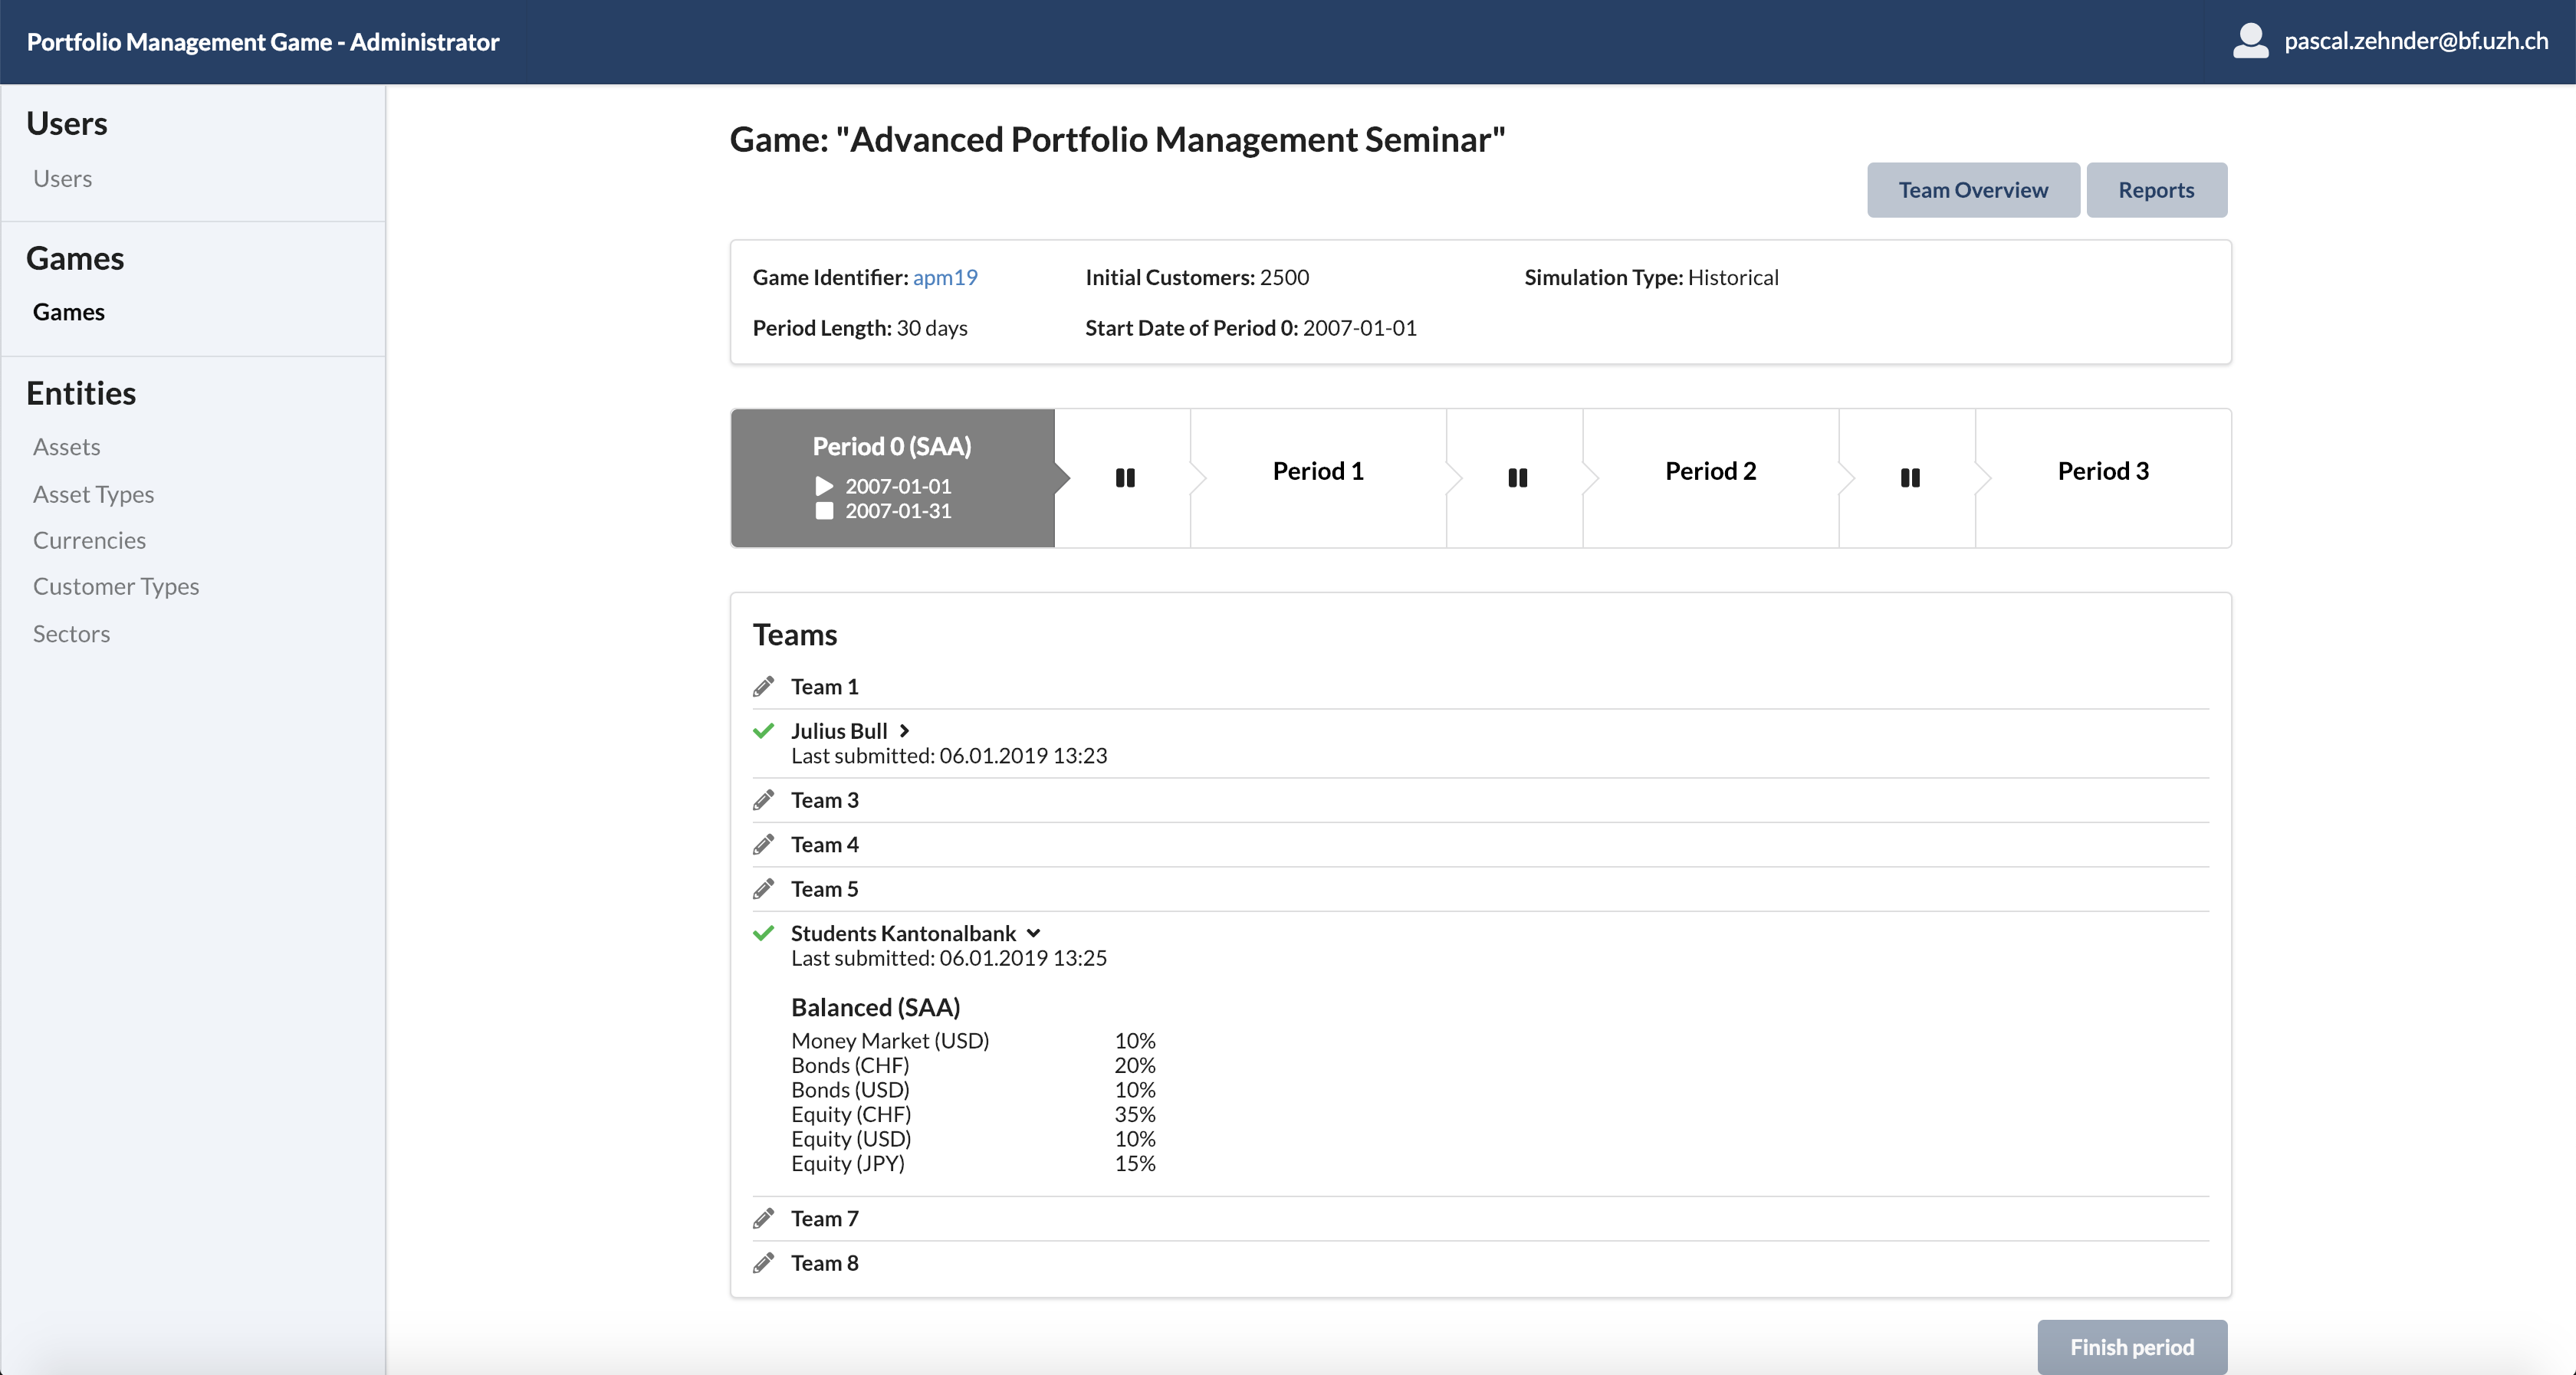
\includegraphics[scale=0.2]{img/application-overview/administrator/07_running_game.png}
  \caption{Running Period Zero}
  \label{fig:running_period}
\end{figure}

\paragraph{Initializing Period One}
After completing period zero, the administrator can continue on to initialize the second period of the game (\Cref{fig:initializing_period}), which is called Period 1. This is the first period that allows students to actually invest and make business decisions. Additionally, new customer types for the next period and other settings could be defined in this phase of the game once period one has been played. New customer types may be added for the next period while all existing ones are not removable. A new customer type has the initial number of customers as defined in the game creation form. Future developments will include additional simulation settings on this screen, which is why the process is separated in two parts (initialization and starting). The simulation would then run between initialization and starting, after which simulation results could be previewed on the starting screen.
% TODO replace with a screen including customer type settings from period 2 e.g.
\begin{figure}[h!]
  \centering
  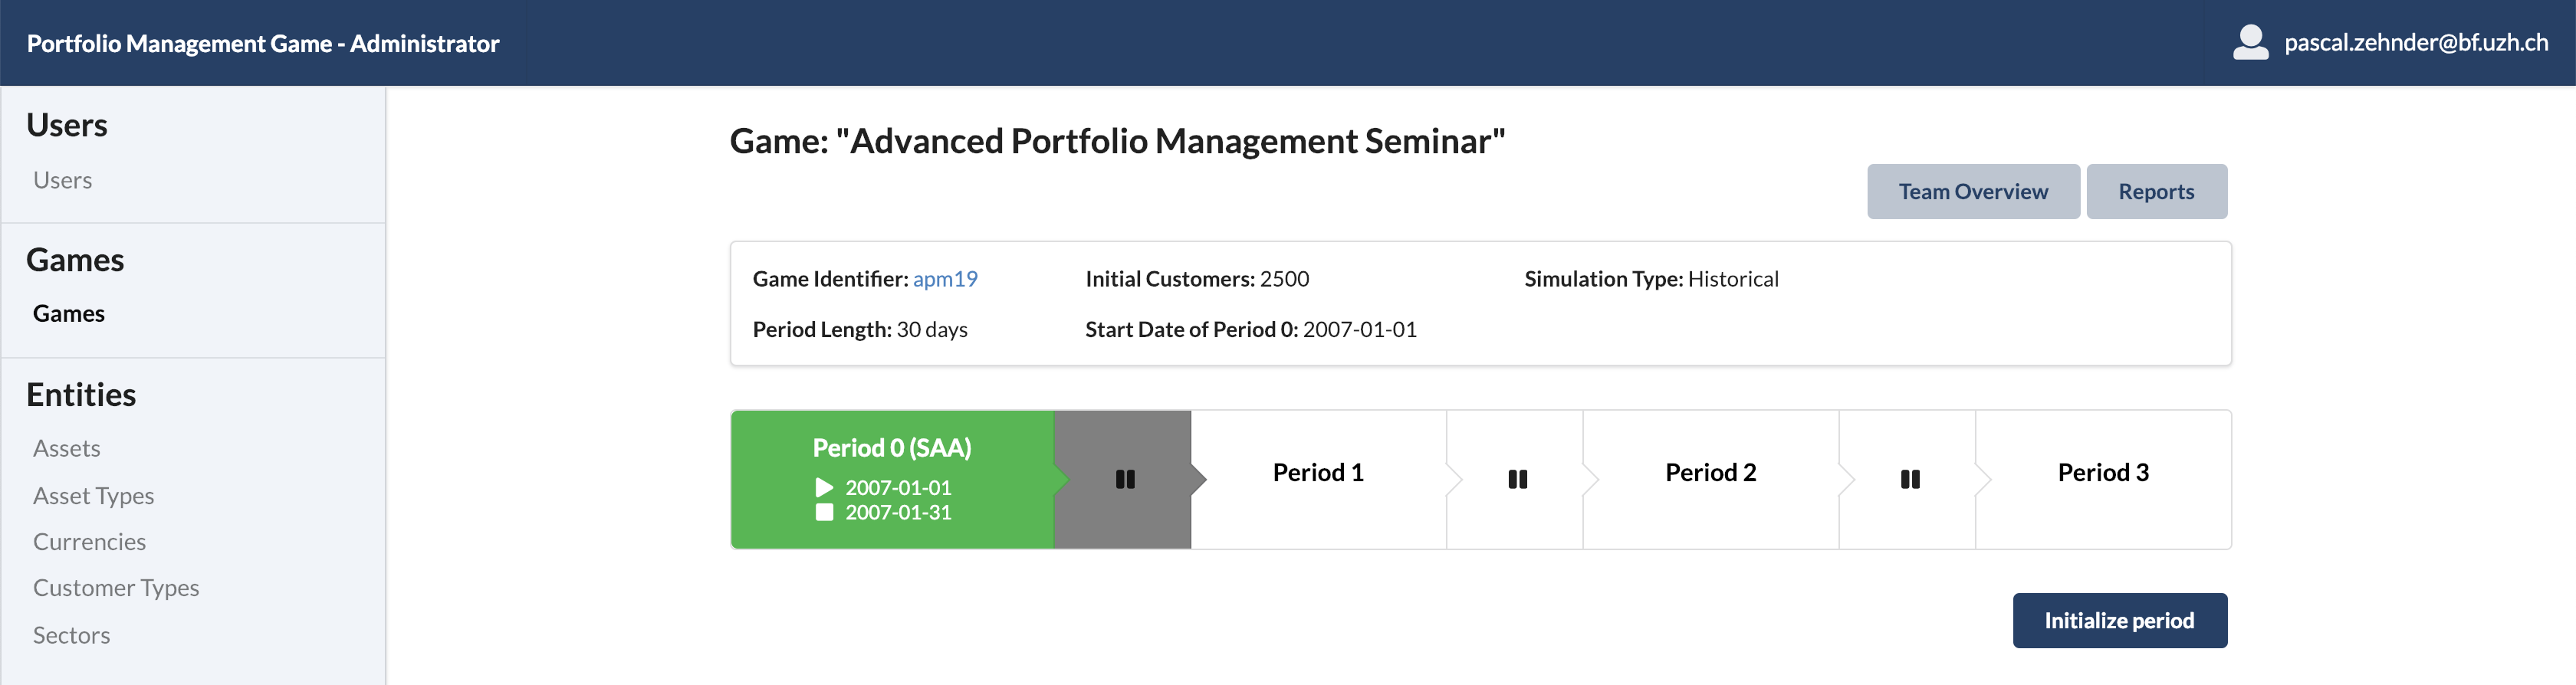
\includegraphics[scale=0.2]{img/application-overview/administrator/08_period_initialization.png}
  \caption{Initialize Period One}
  \label{fig:initializing_period}
\end{figure}

\paragraph{Start Period One}
After initializing the next period of a game, the administratos can define some messages (same as in period zero / game initialization, \Cref{fig:starting_period_one}). On starting the next period, teams can then define their decisions as described for the previous screen.
\begin{figure}[h!]
  \centering
  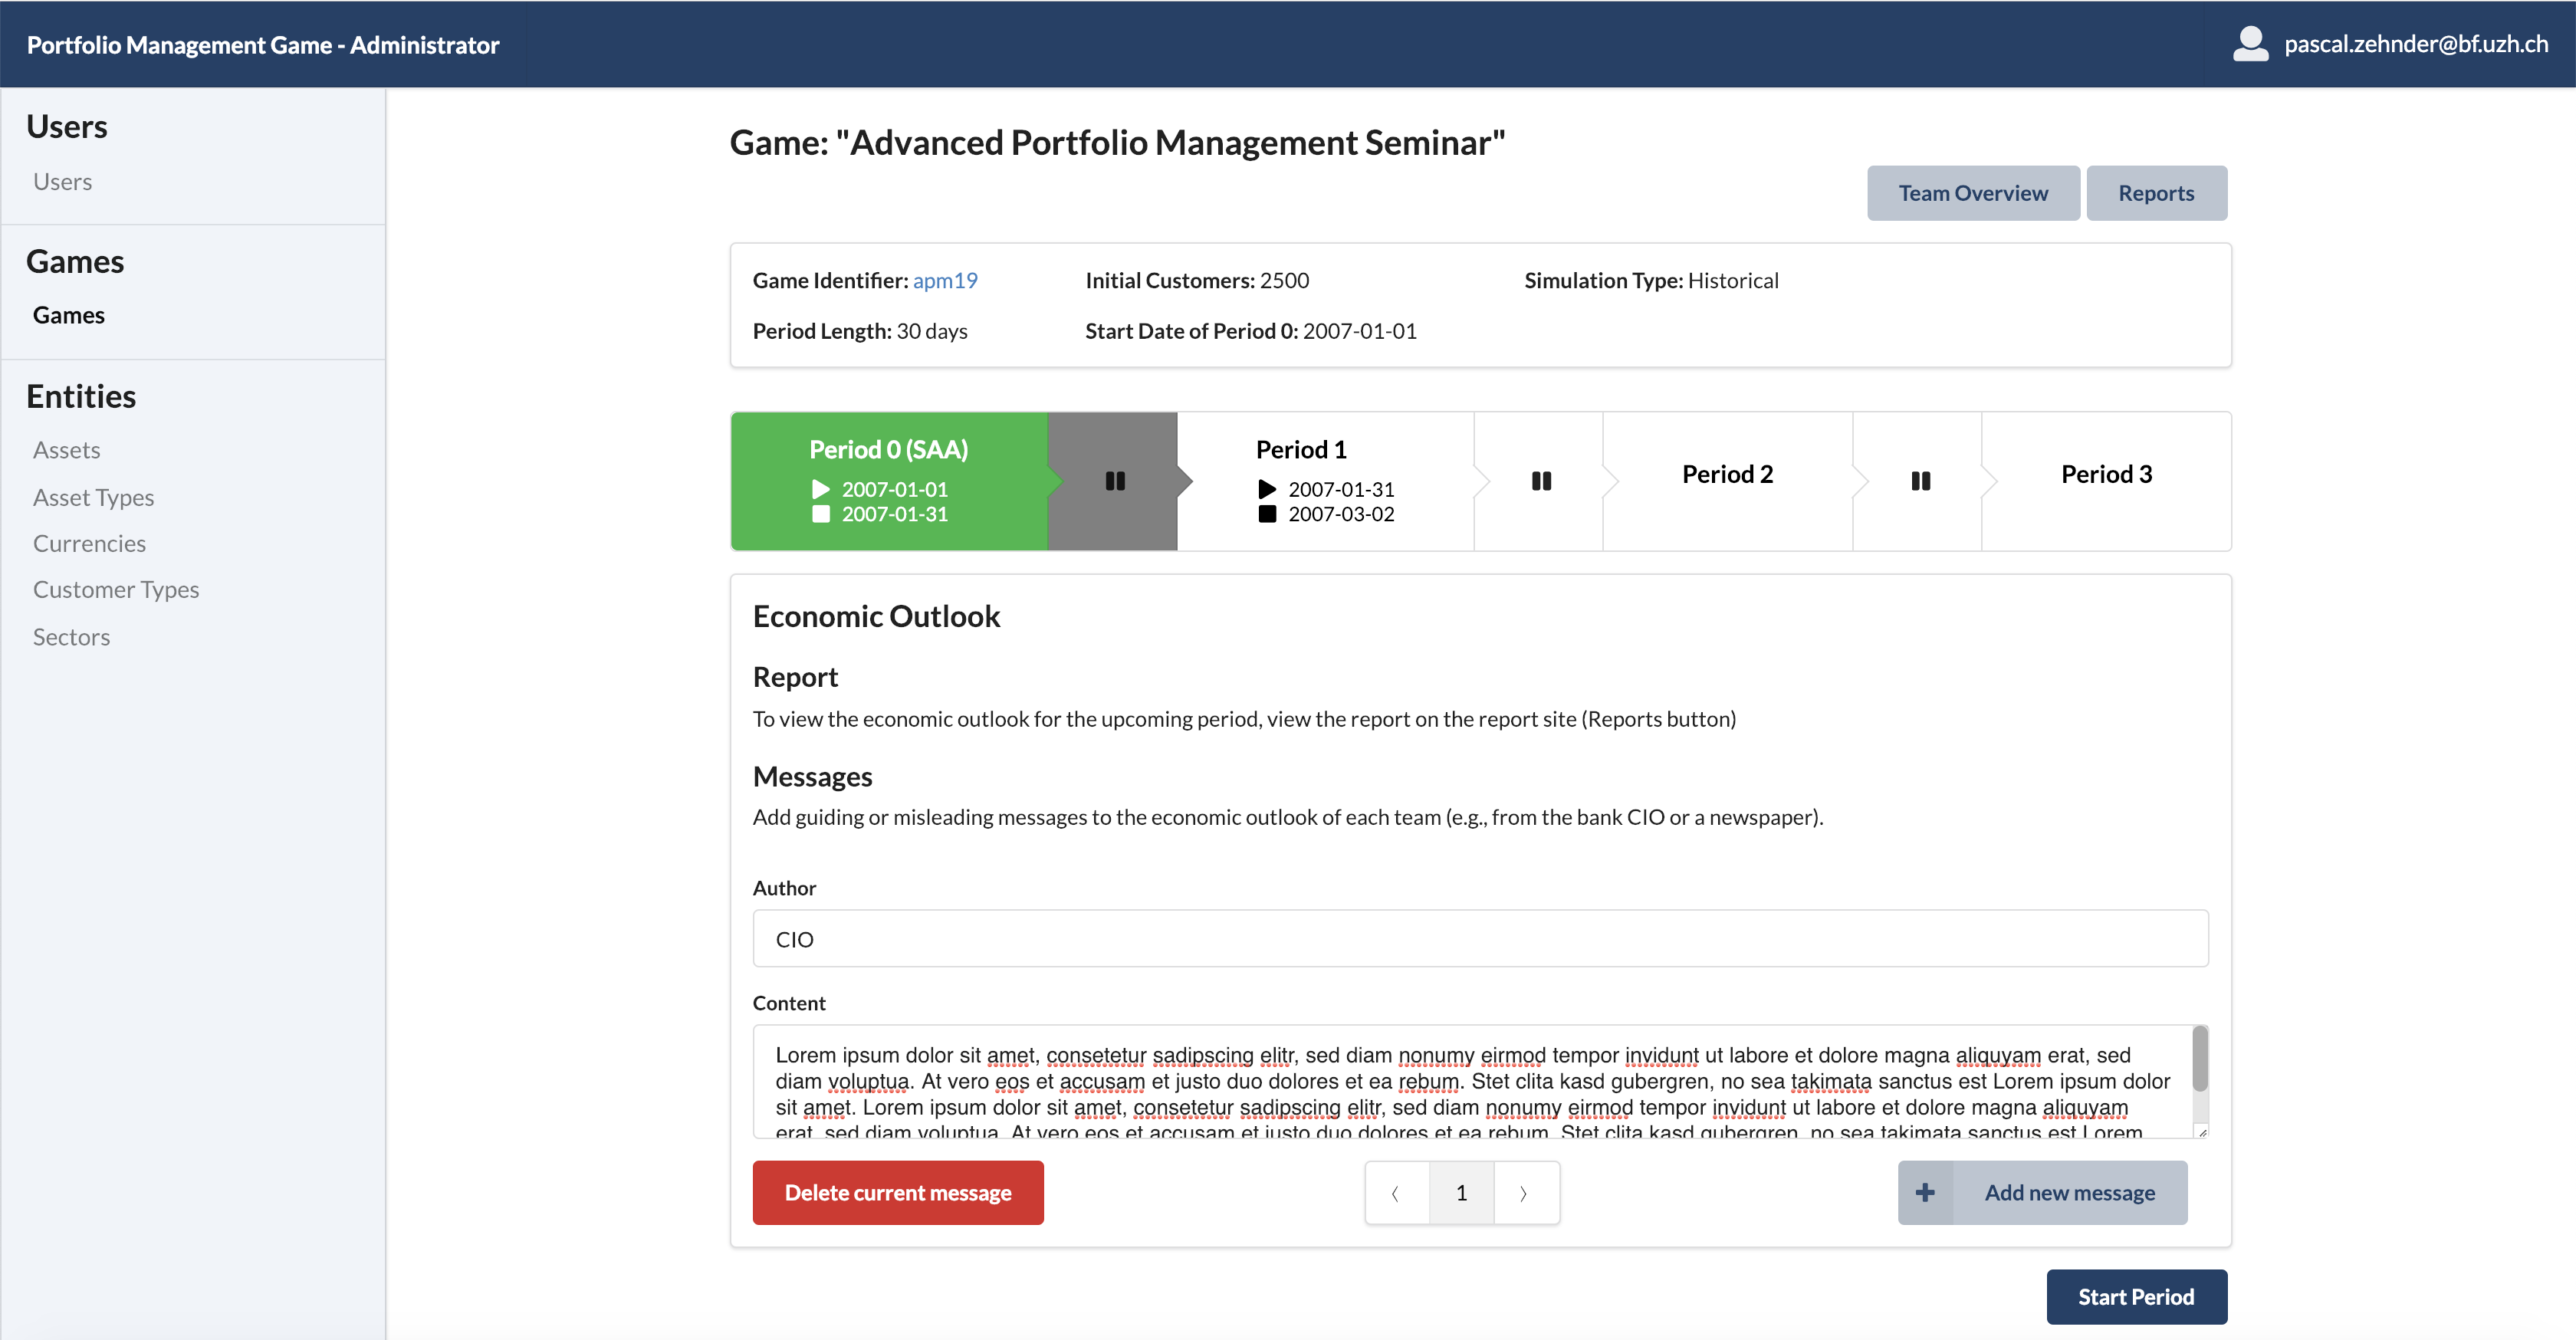
\includegraphics[scale=0.2]{img/application-overview/administrator/09_period_start.png}
  \caption{Start Period One}
  \label{fig:starting_period_one}
\end{figure}

\paragraph{Reports}
For the presentation of the team results in between two running periods, a reporting screen is accessible to the administrator. A detailed description can be found in \Cref{subsec:reports}, as the teams access the same reports as the administrator of that running game.


\subsubsection{Entities Administration}

\paragraph{Assets}
All assets are visible within this page which are available for all game masters, as visible in \Cref{fig:assets}. They can be synchronized with the InfluxDB database to reflect the current contents of the database. When synchronizing those assets, they will be updated for all users.
\begin{figure}[h!]
  \centering
  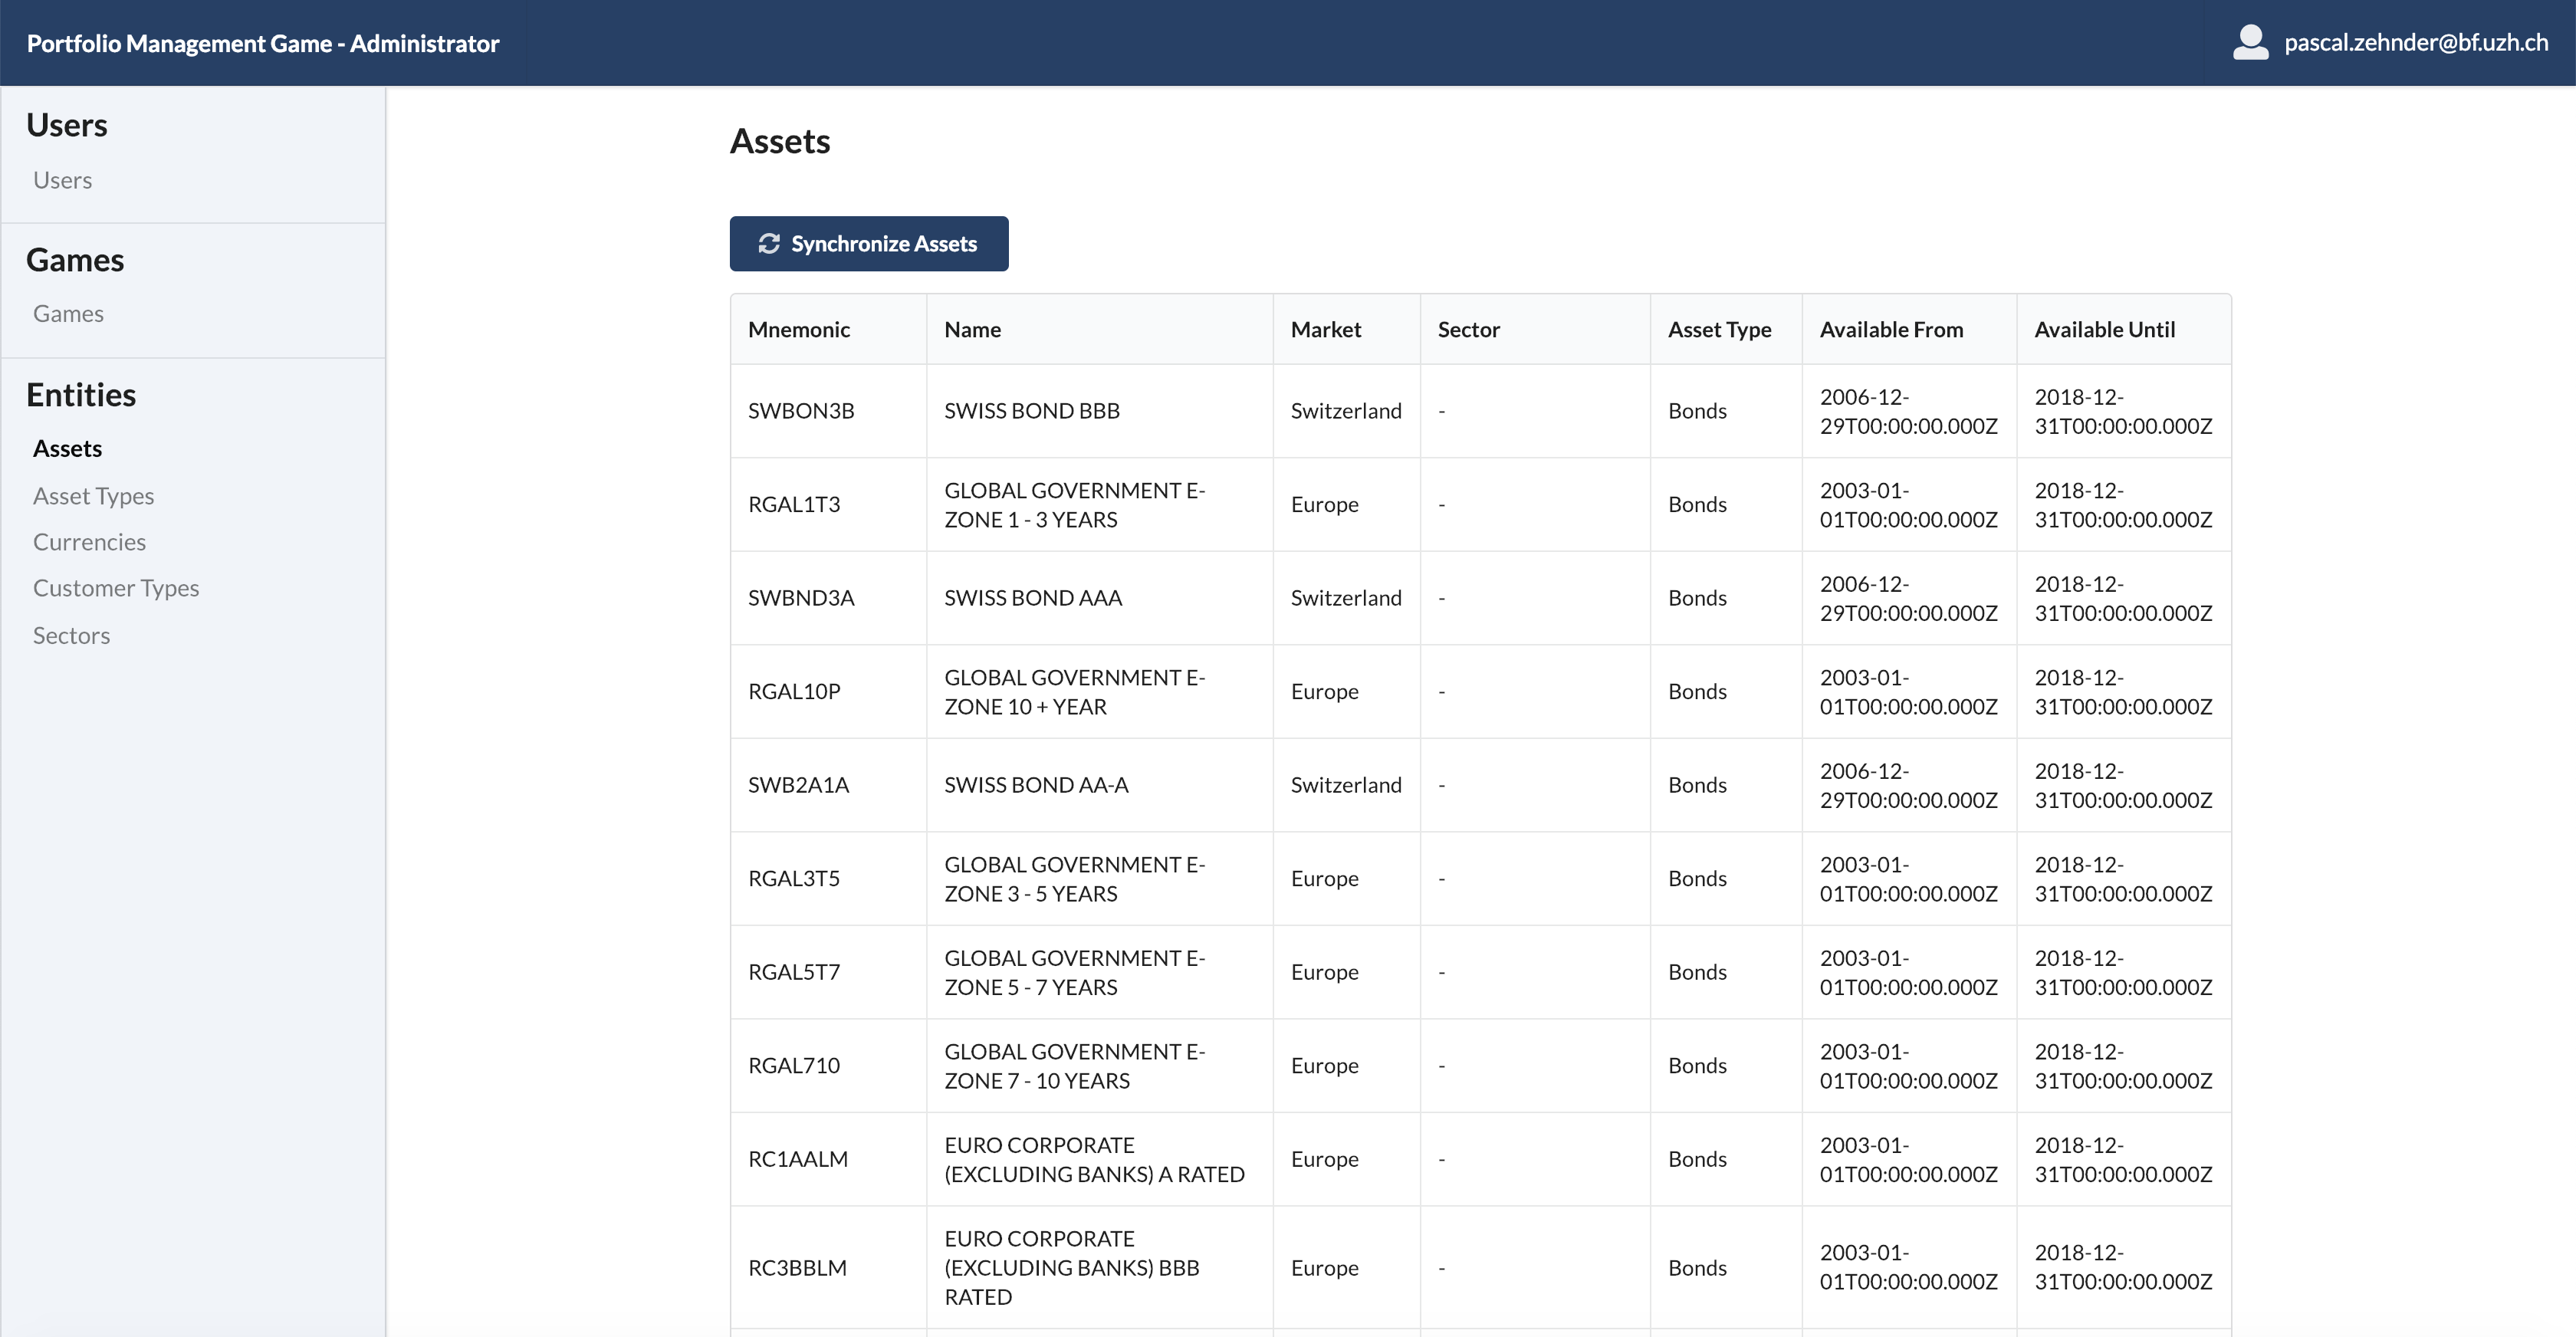
\includegraphics[scale=0.2]{img/application-overview/administrator/entities_assets.png}
  \caption{Assets Administration}
  \label{fig:assets}
\end{figure}


\paragraph{Asset Types}
A table showing all asset types that may be edited is the landing page of this entity. By editing a specified asset type, the administrator can change some characteristics of its type, such as info text as shown in \Cref{fig:asset_types}.
\begin{figure}[h!]
  \centering
  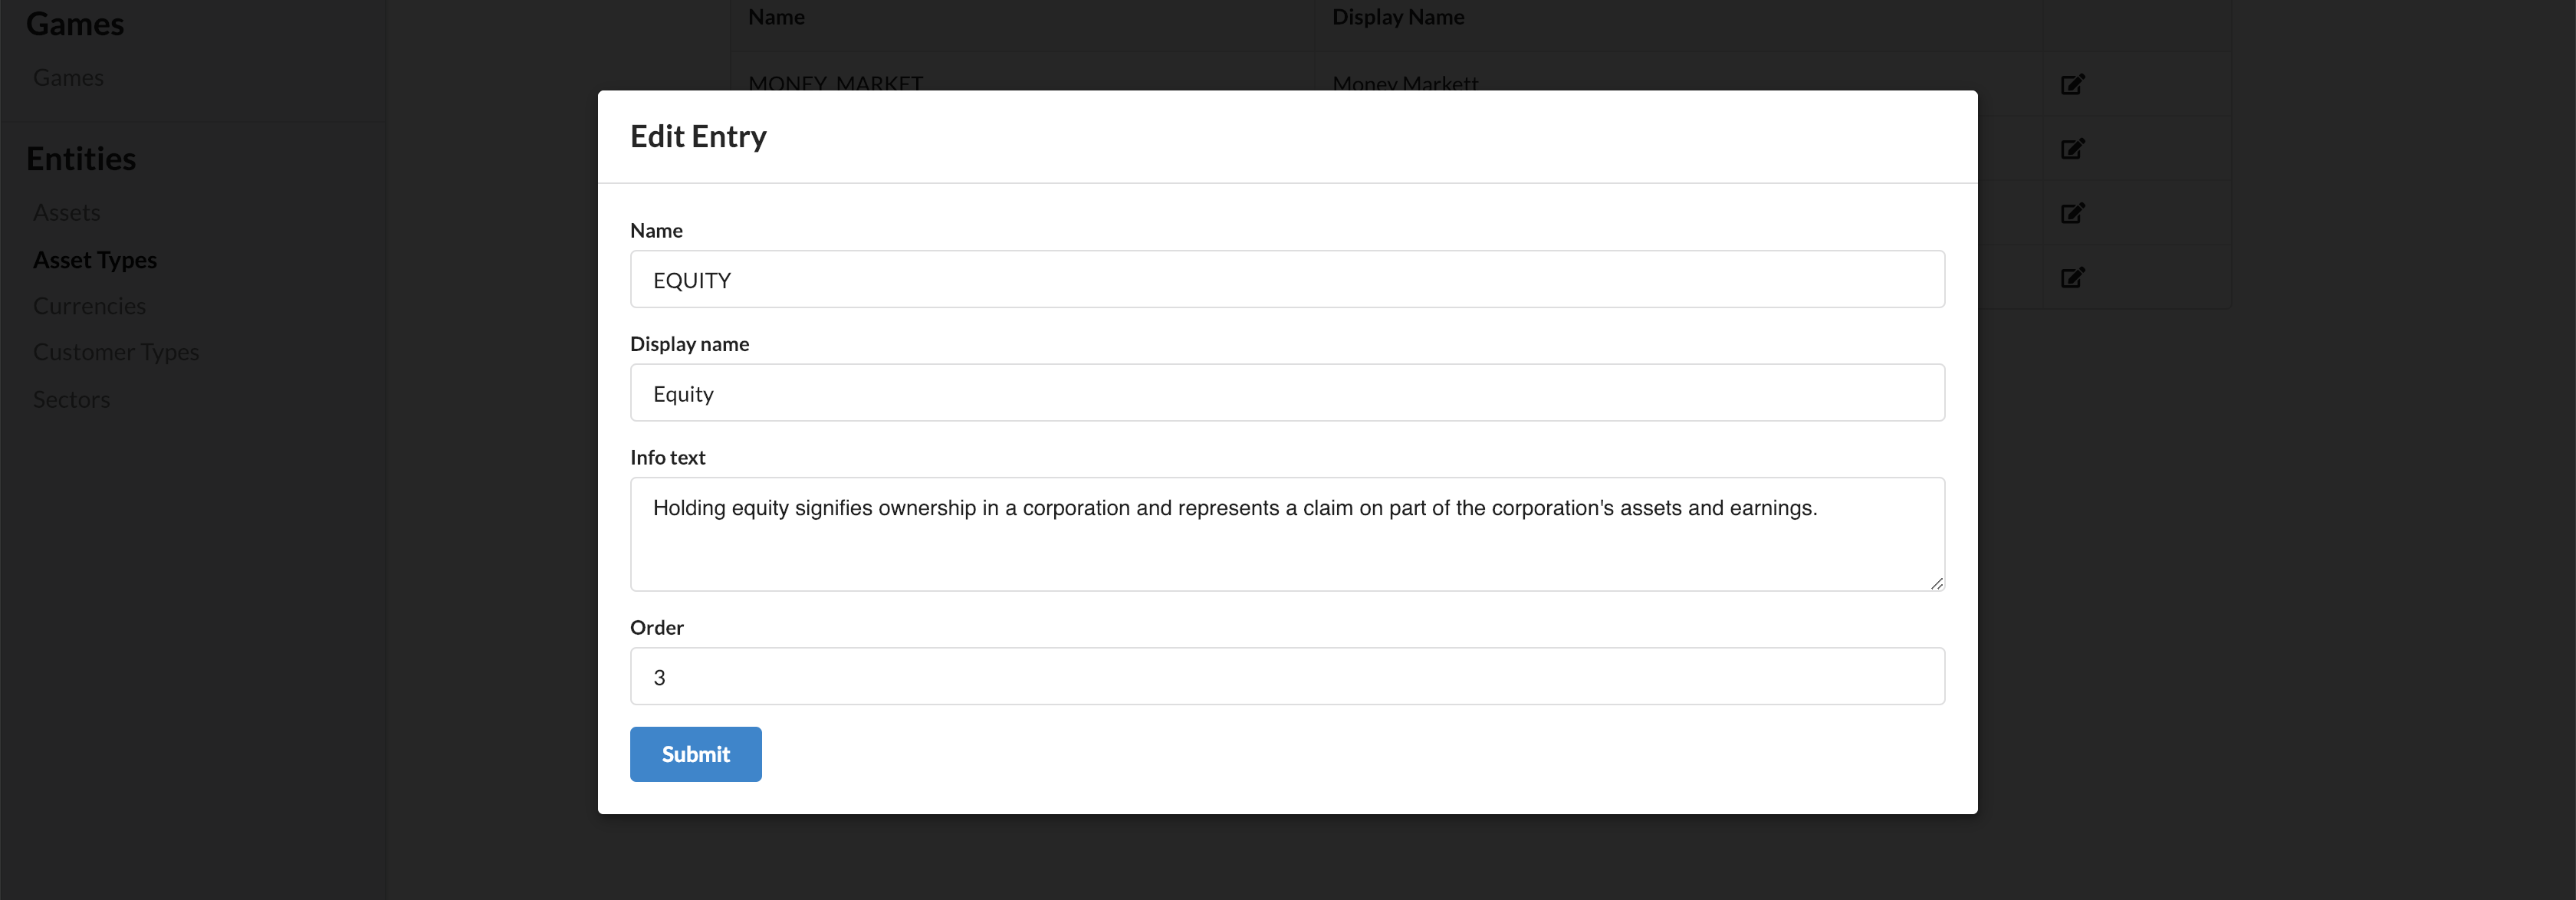
\includegraphics[scale=0.2]{img/application-overview/administrator/entities_asset_types.png}
  \caption{Asset Types Administration}
  \label{fig:asset_types}
\end{figure}

\paragraph{Currencies}
The currencies may be edited in the same manner as the asset types. By submitting changes, the displaying name or symbol of the corresponding currency will be edited.

\paragraph{Customer Types}
An overview of all available customer types is provided for the administrator. For each customer type, the ideal strategic asset allocation and the ranges for currencies and asset types (both dimensions) can be modified. Additionally, the info bullets and the displaying name may be modified. \Cref{fig:customer_types} shows the embedded allocation table with its ranges and the customer type's ideal SAA.

\begin{figure}[h!]
  \centering
  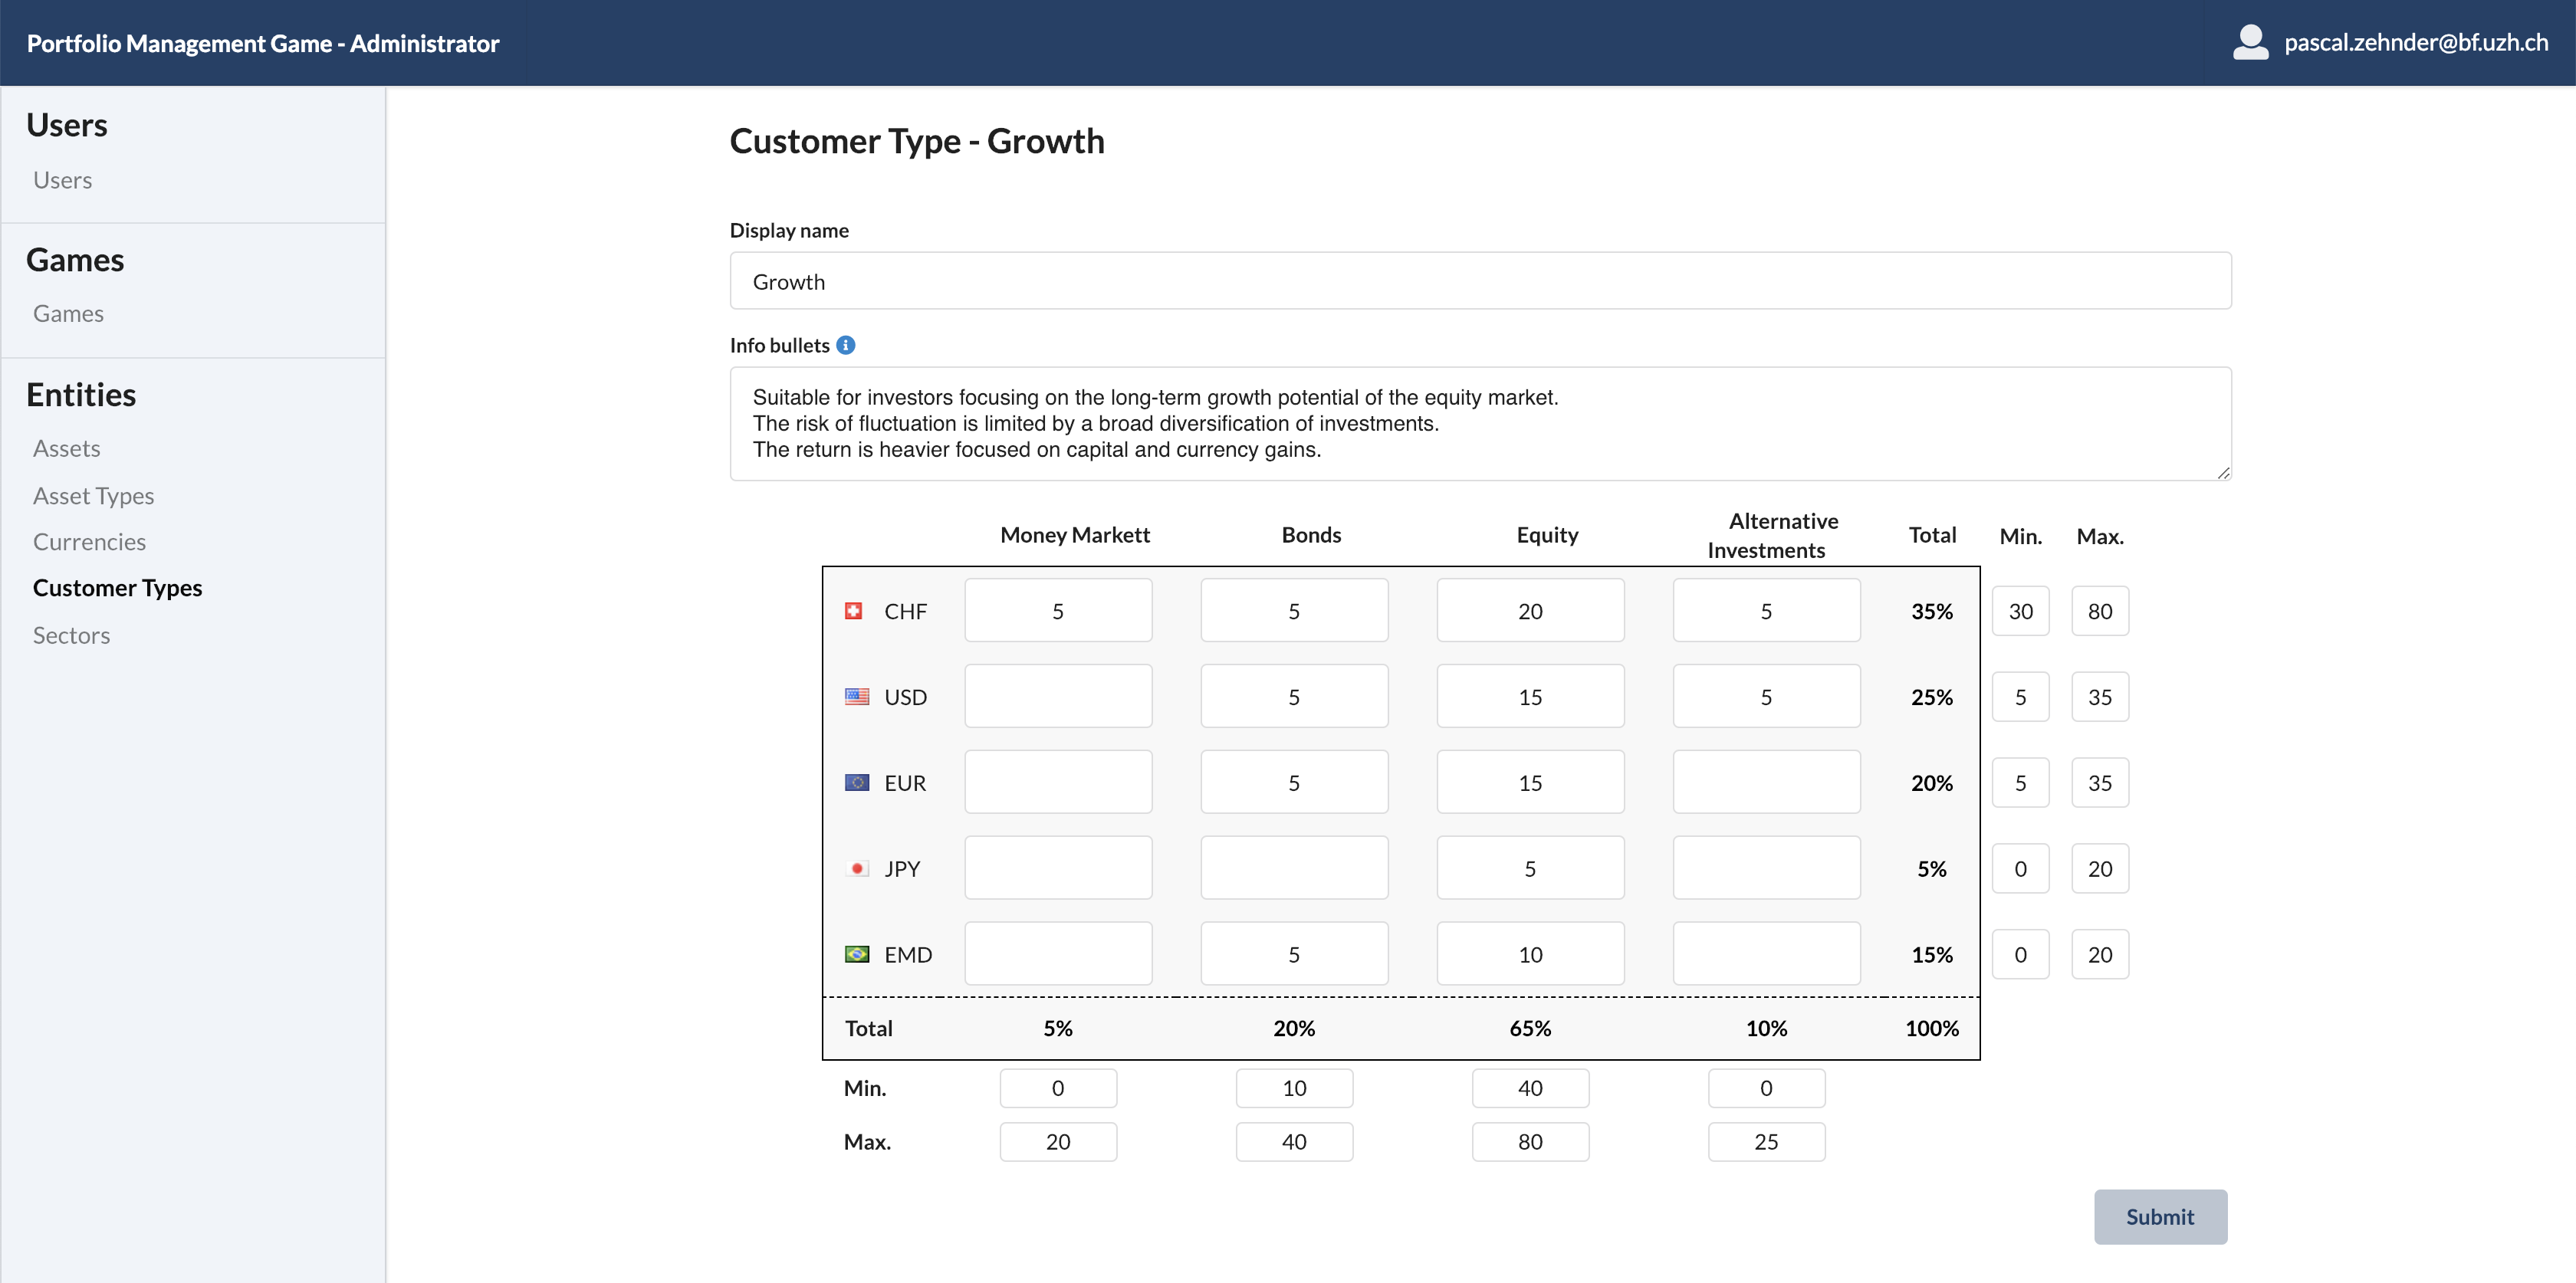
\includegraphics[scale=0.2]{img/application-overview/administrator/entities_customer_types.png}
  \caption{Customer Types Administration}
  \label{fig:customer_types}
\end{figure}

\paragraph{Sectors}
A short overview of all sectors which are used in the asset page when synchronizing all assets.


\subsection{Team Views}

\subsubsection{Team Login}
When accessing the landing page, a team has to input a game short id as provided by the administrator. Afterward, the team has to log in with valid credentials to participate within a game (\Cref{fig:team_login}). Teams are informed about possible inconsistencies when logging in on multiple devices and submitting their current decisions.
\begin{figure}[h!]
  \centering
  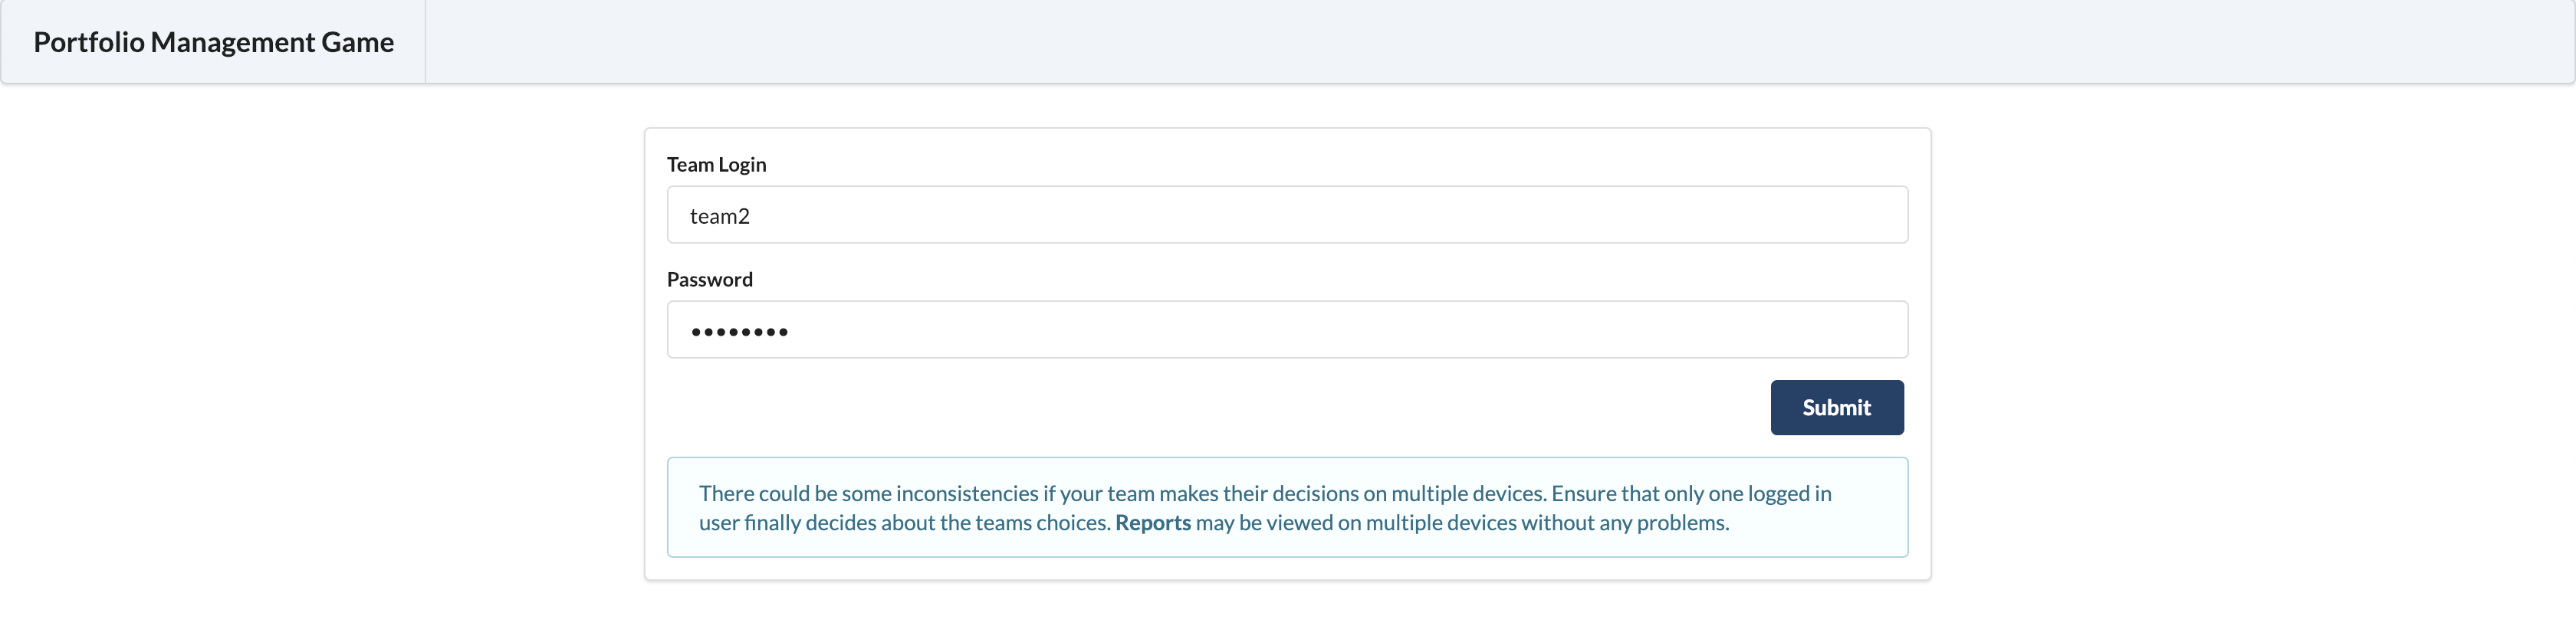
\includegraphics[scale=0.2]{img/application-overview/teams/01_login.png}
  \caption{Team Login}
  \label{fig:team_login}
\end{figure}

\subsubsection{SAA}
In period 0, which represents phase 1 of the game, the teams define their SAA for all customer types which are enabled by the administrator of the specific game (\Cref{fig:saa_decisions}). The teams need to fulfill the type and currency constraints for all dimensions to submit their decisions. Supportive graphs in form of pie charts help the teams to decide about the share of the two dimensions. Additionally, the players can name their team on the top left corner of the screen, but do not have to do so.
\begin{figure}[h!]
  \centering
  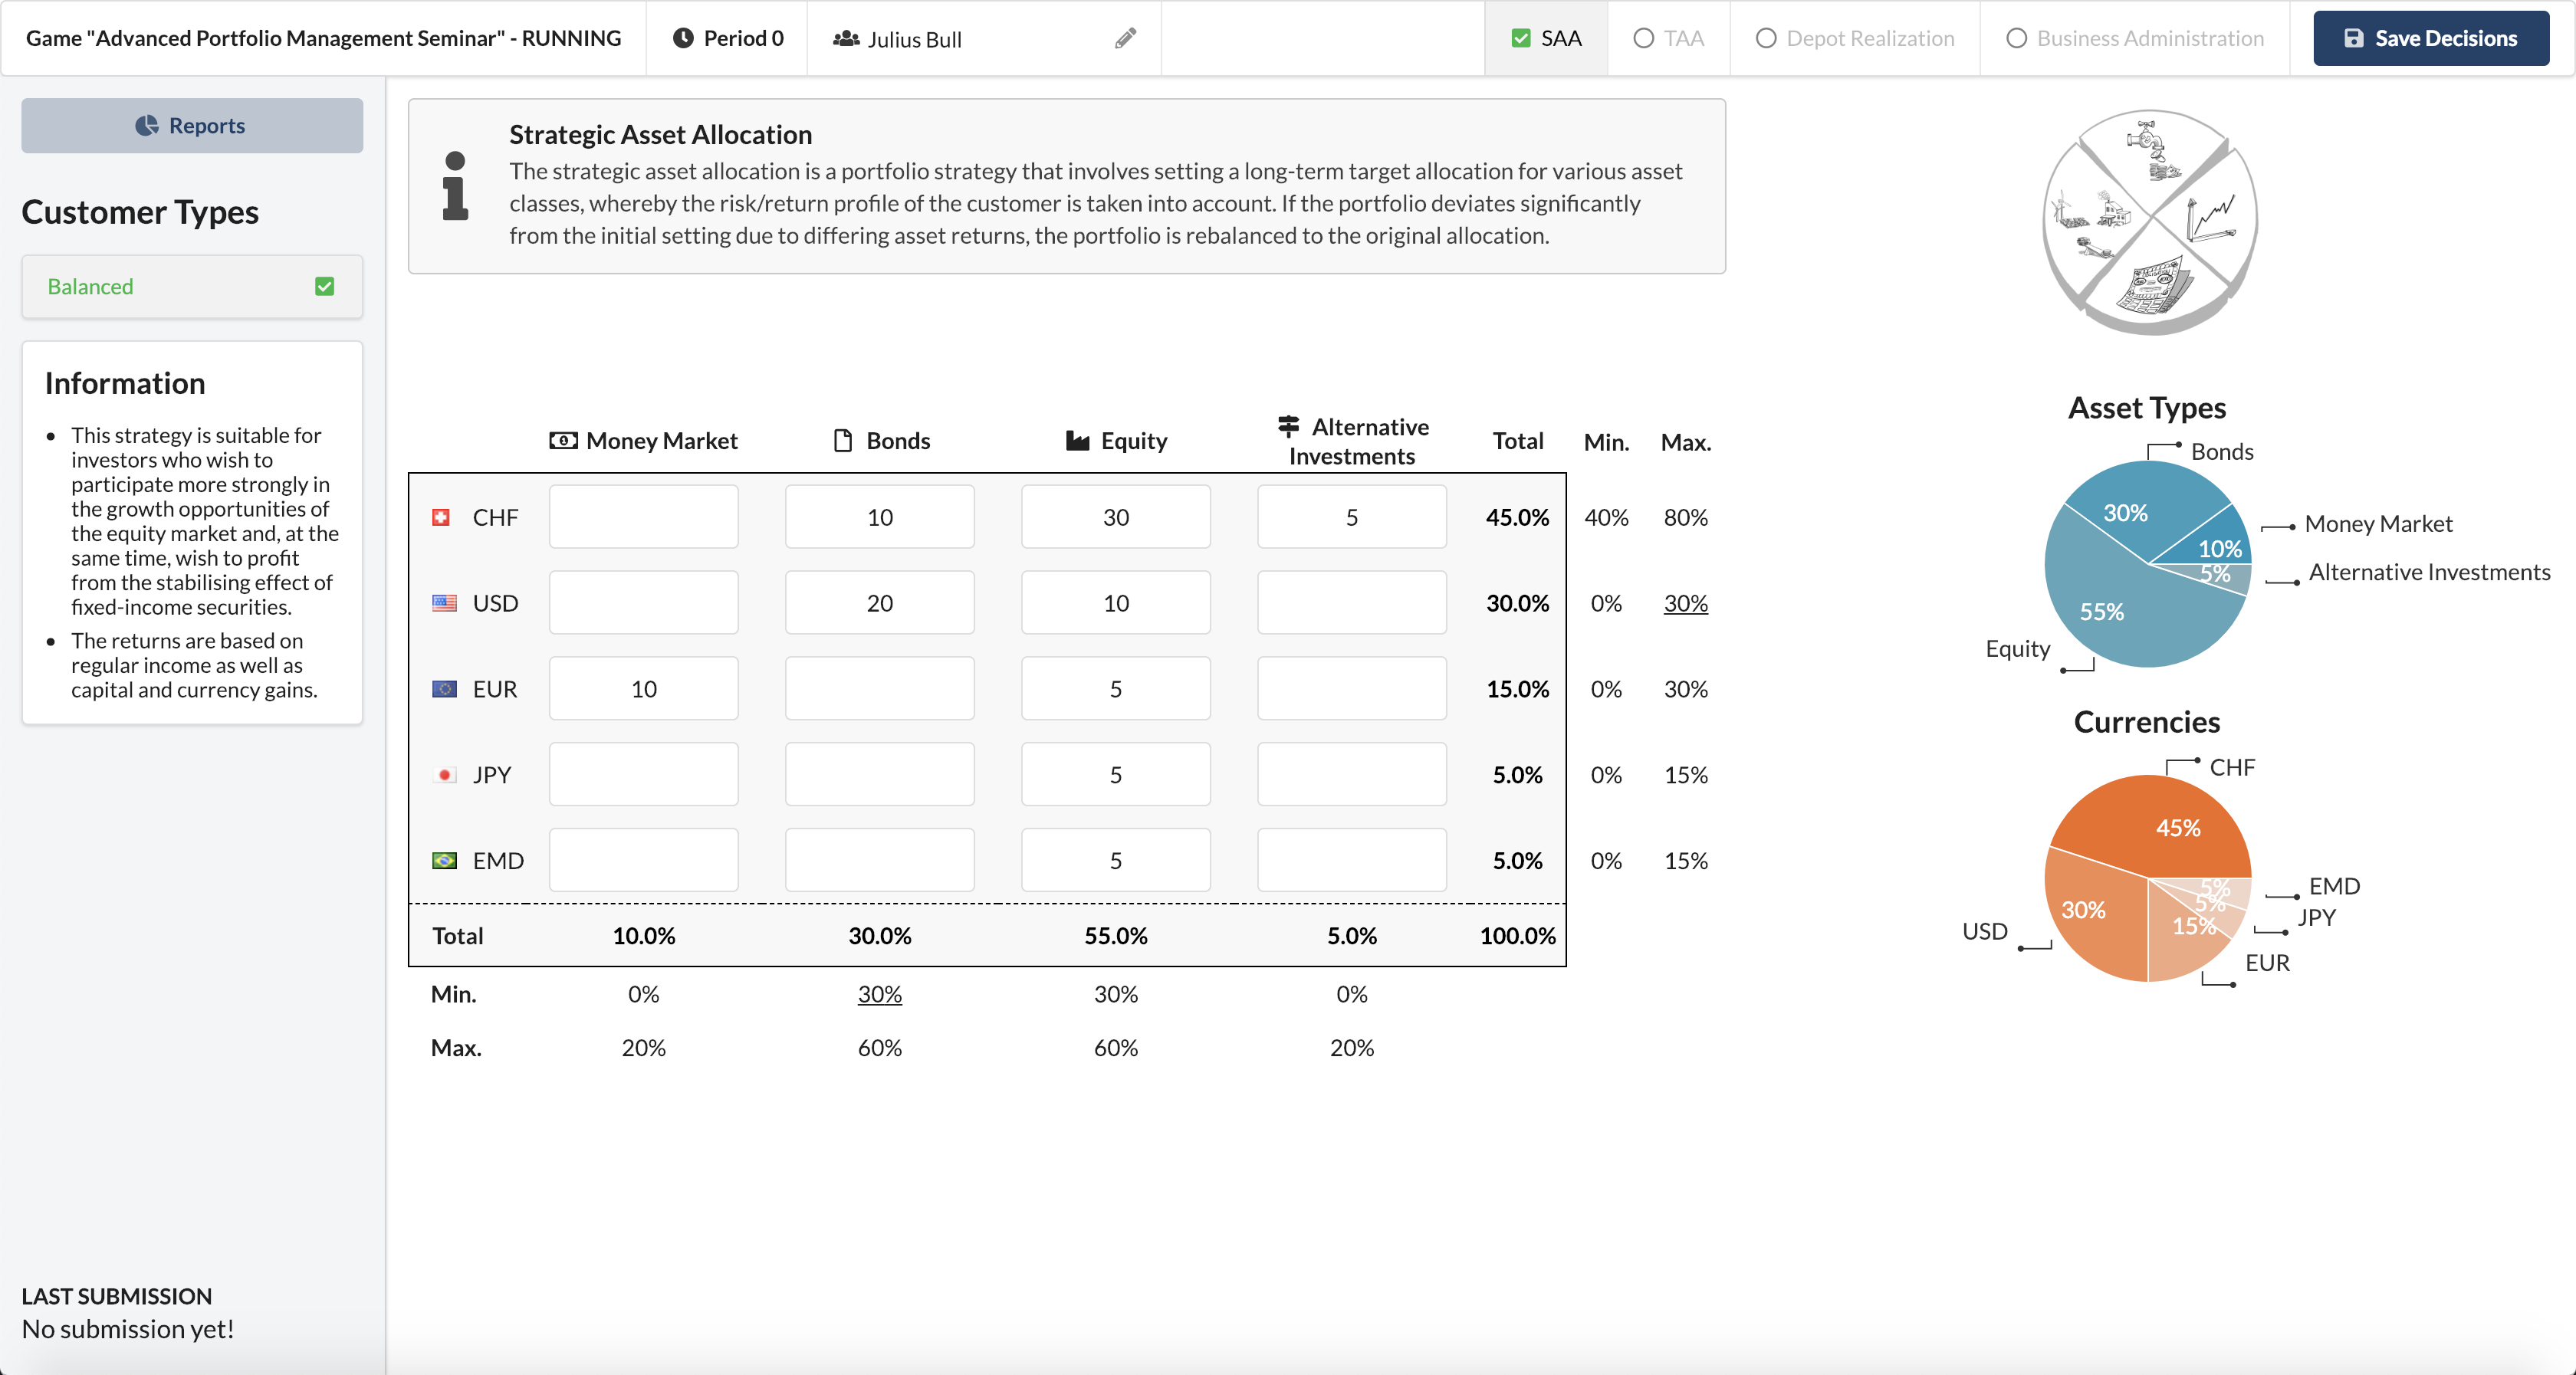
\includegraphics[scale=0.2]{img/application-overview/teams/02_period_zero_decisions.png}
  \caption{SAA Decisions in Period Zero}
  \label{fig:saa_decisions}
\end{figure}

\subsubsection{TAA}
Starting from period 1, a team has to complete multiple decisions separated into four pages. Strategic asset allocation is fixed and not editable for a customer type which was defined at the beginning of the game. When the administrator defines a new customer type for an upcoming period, the teams have to allocate both SAA and TAA for the new customer type. For each step within this process, a progress state helps the teams to understand the state of each step. For saving their decisions, all four steps have to be completed. In the bottom left corner, the submission state may be seen. \\

For the tactical asset allocation, the teams can deviate from the SAA based on their expectations on changes in the overall market. Equal to the strategic asset allocation screen, teams change the input within the table and get illustrative support with two graphs, displaying the allocations for both dimensions of the table (\Cref{fig:taa_decisions}). Initially, the inputs from the strategic asset allocation are loaded, whereas the students can adjust them to market changes. Arrows within the total summation of each asset type or currency show the status of being within the range of the current customer type.
\begin{figure}[h!]
  \centering
  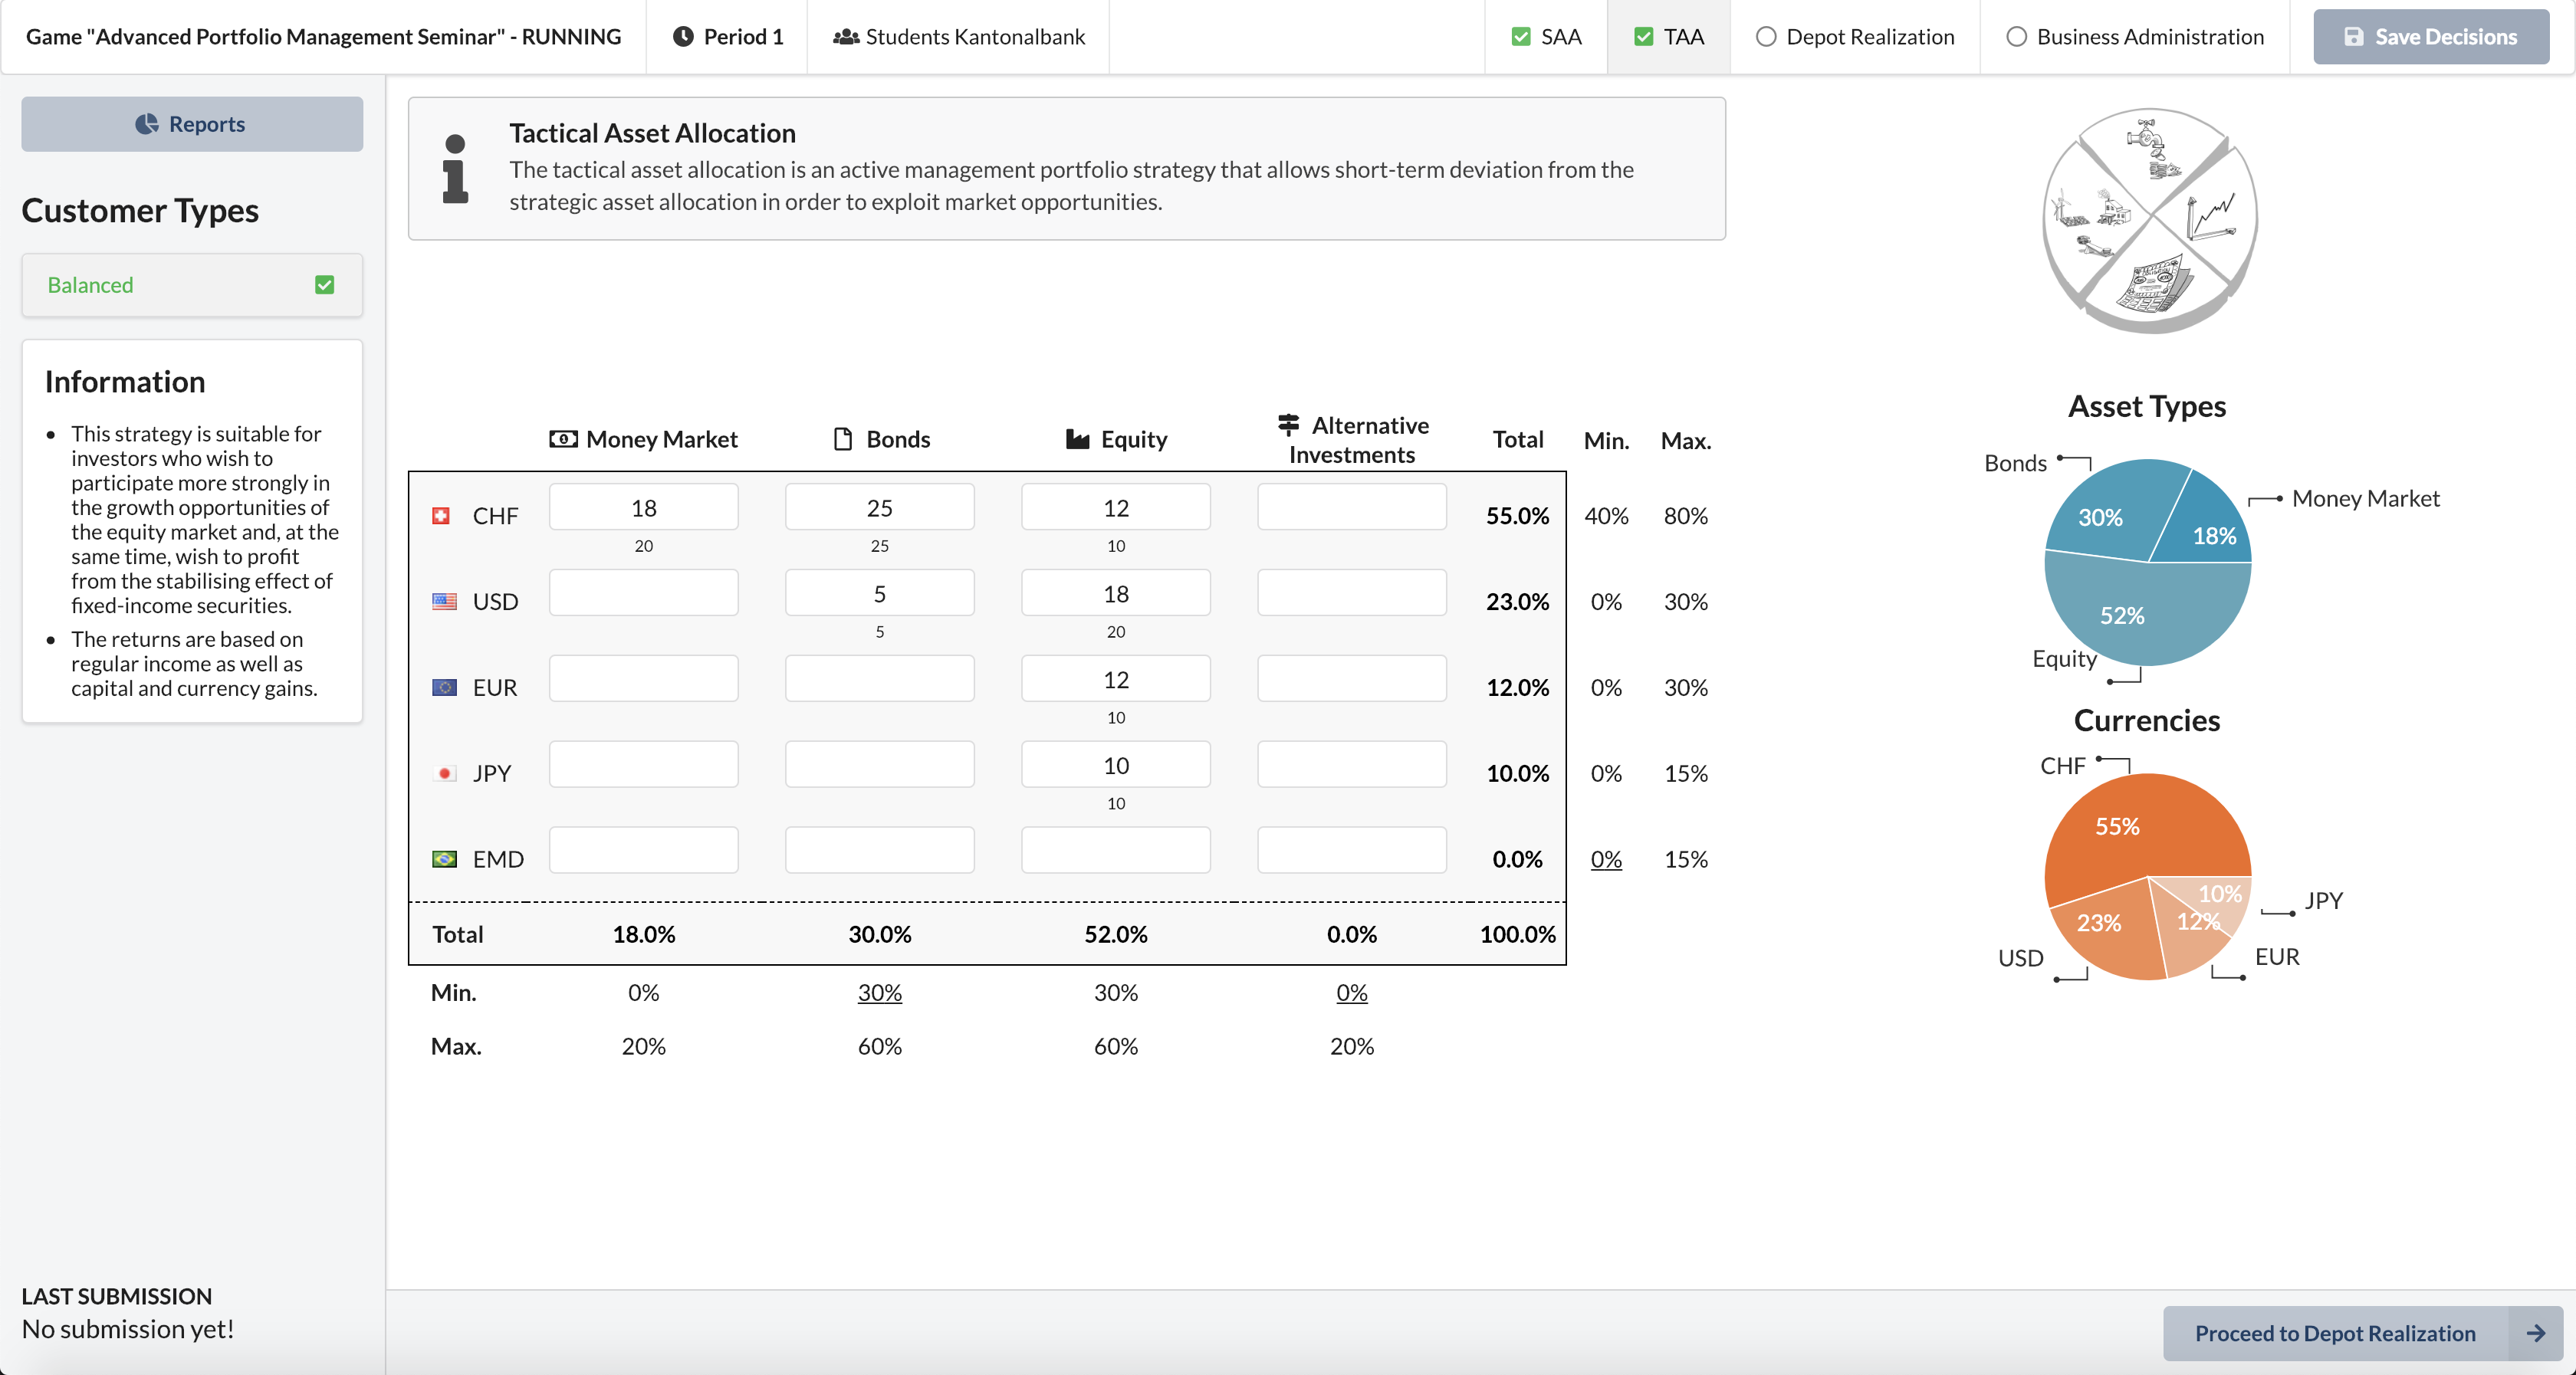
\includegraphics[scale=0.2]{img/application-overview/teams/04_taa.png}
  \caption{TAA Decisions in Periods > 0}
  \label{fig:taa_decisions}
\end{figure}

\subsubsection{Depot Realization}
Based on SAA and TAA, the teams finally have to allocate their money in specific assets. By having bar charts on the top of the screen, students have an overview of their SAA and TAA decisions of the current active customer type. A target for the students is to allocate assets such that the yellow realization bar aligns with TAA for each asset type/currency combination. On the top right corner, a short summary of the most important key numbers for the allocations is present. This process has to be repeated for each customer type defined by navigating on the left menu. Equal to the SAA and TAA screen, the progress of the customer types is highlighted with checkmarks and corresponding colors \Cref{fig:depot_realization}.

\begin{figure}[h!]
  \centering
  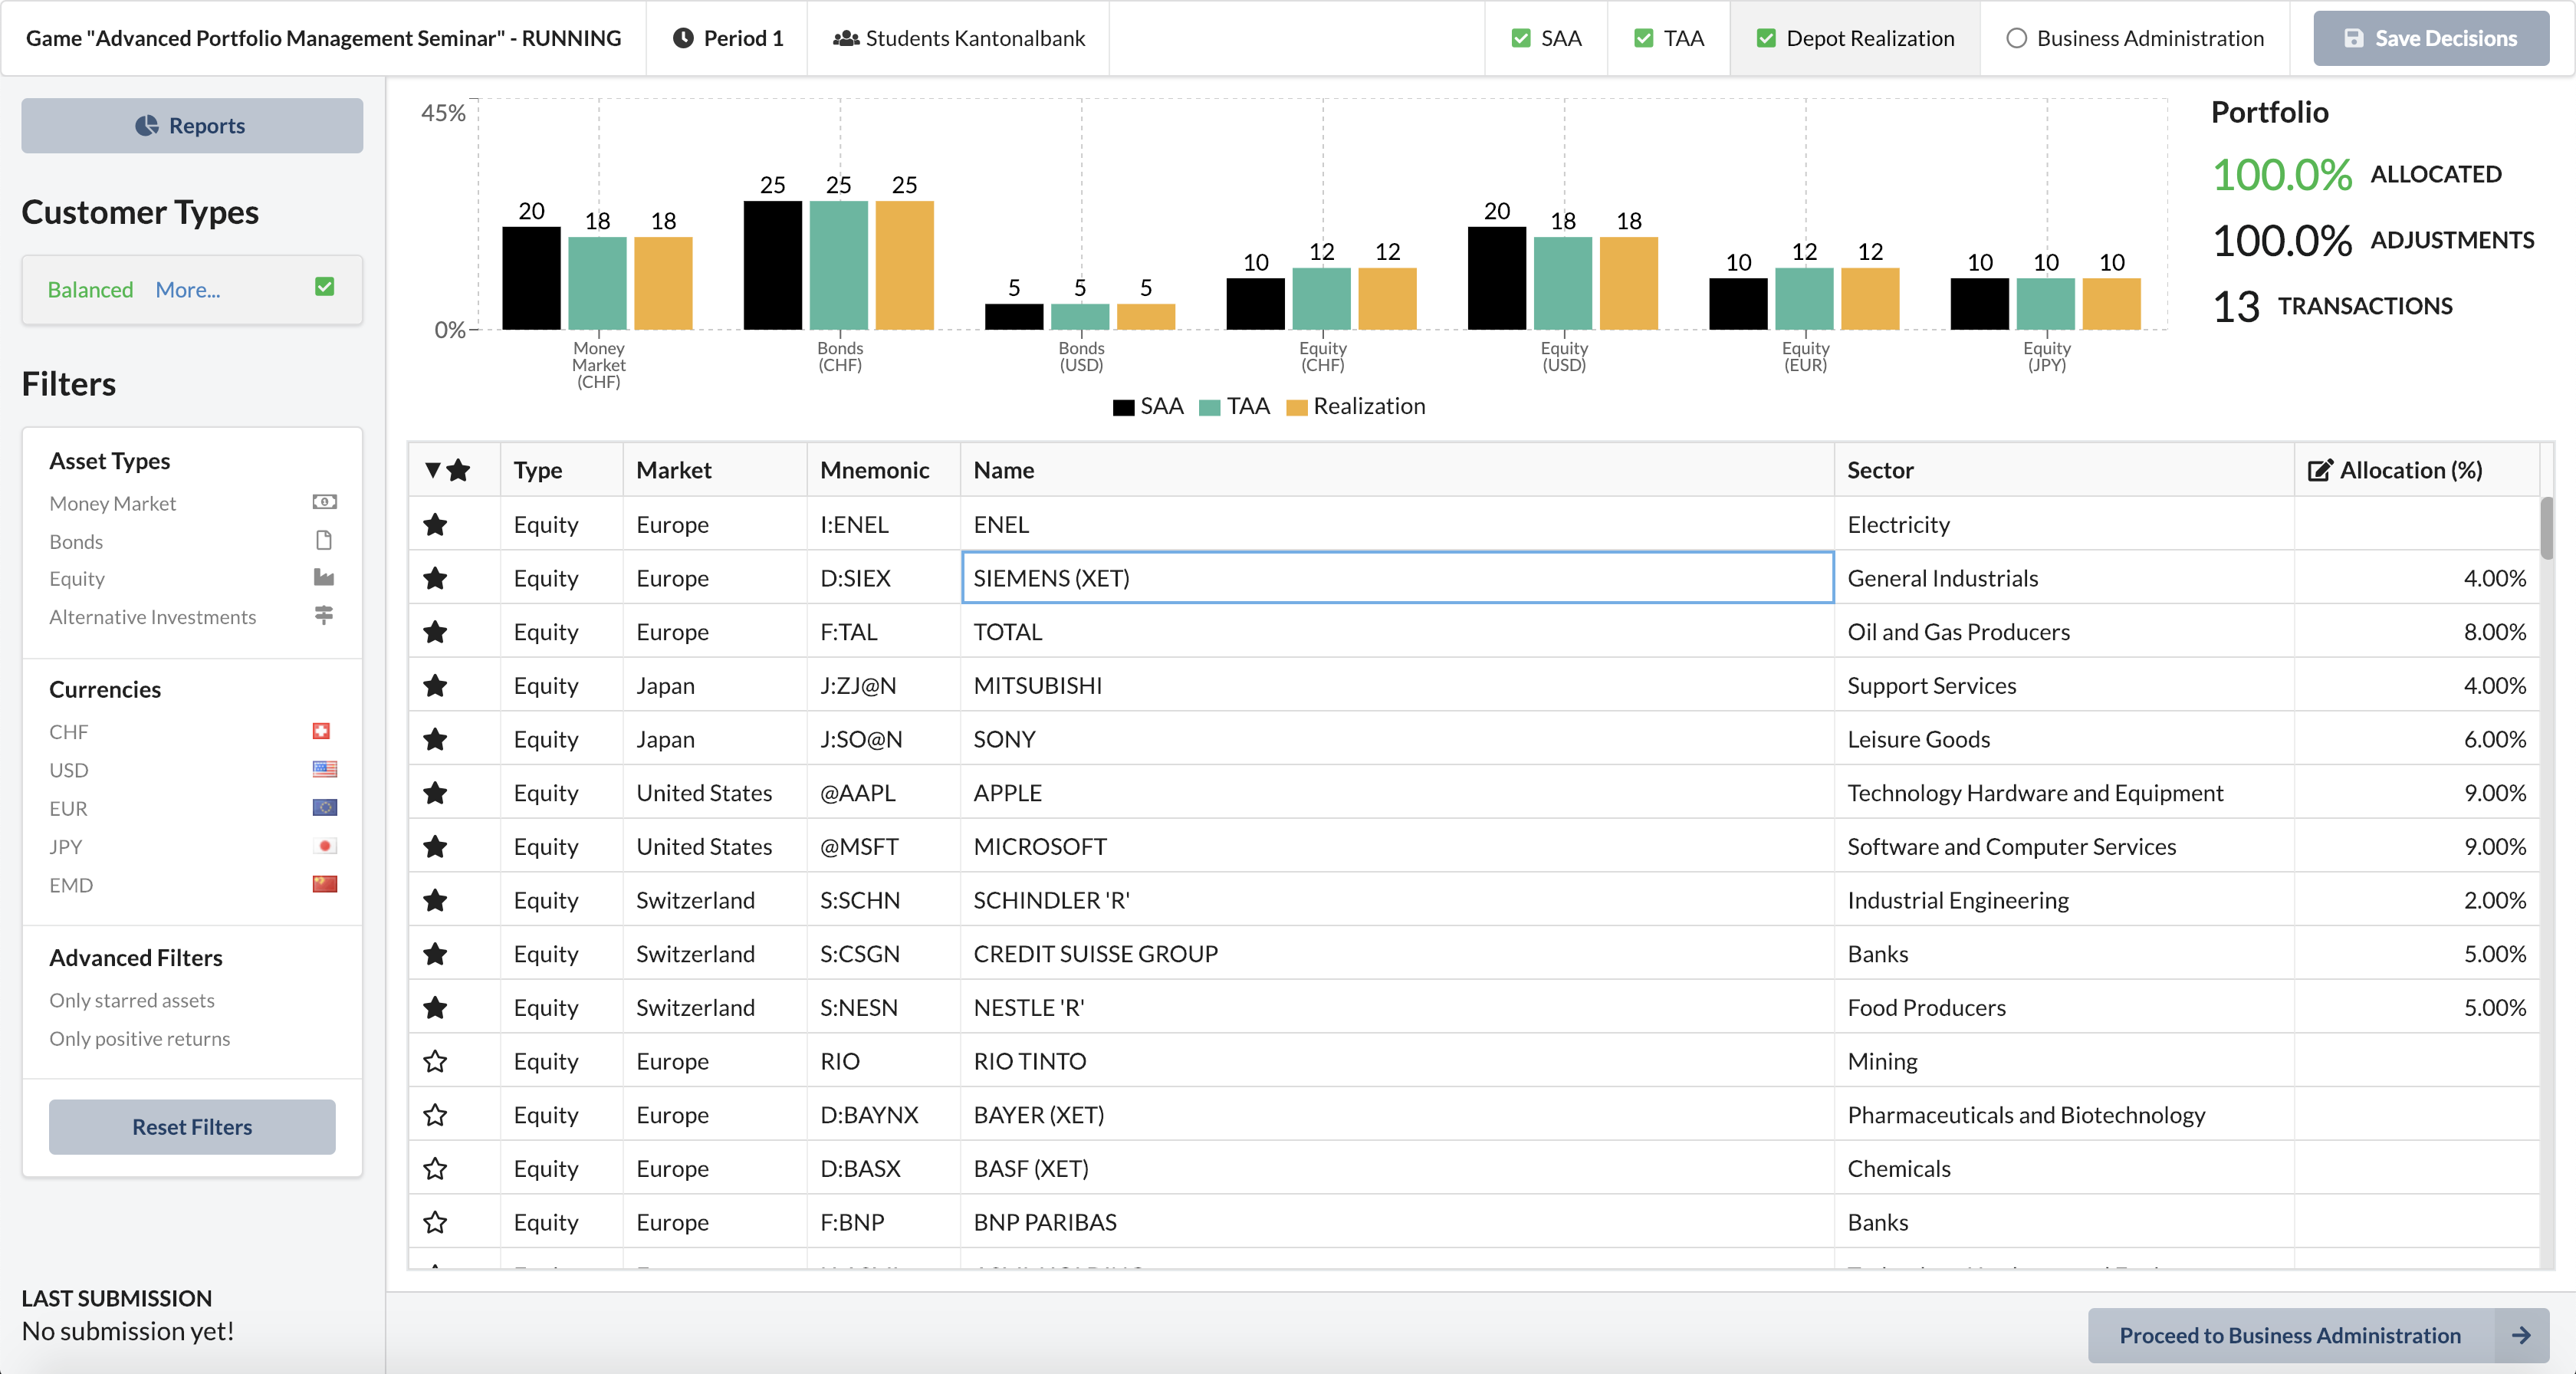
\includegraphics[scale=0.2]{img/application-overview/teams/05_depot_realization.png}
  \caption{Depot Realization}
  \label{fig:depot_realization}
\end{figure}

\subsubsection{Business Administration}
Business administration decisions are the final set of decisions made in a period \Cref{fig:business_admin}. On the left side of the screen, teams can input numbers for four different categories of decisions: conditions \& fees, hHuman resources, logistics, and profit distribution. For each input field, an initial value (in period 1) or the previous period value (for all other periods) is displayed next to the input field. On the right side of the page, the balance sheet from the previous period is visualized to inform teams about their business results. Further key information is displayed on top of the balance sheet.
\begin{figure}[h!]
  \centering
  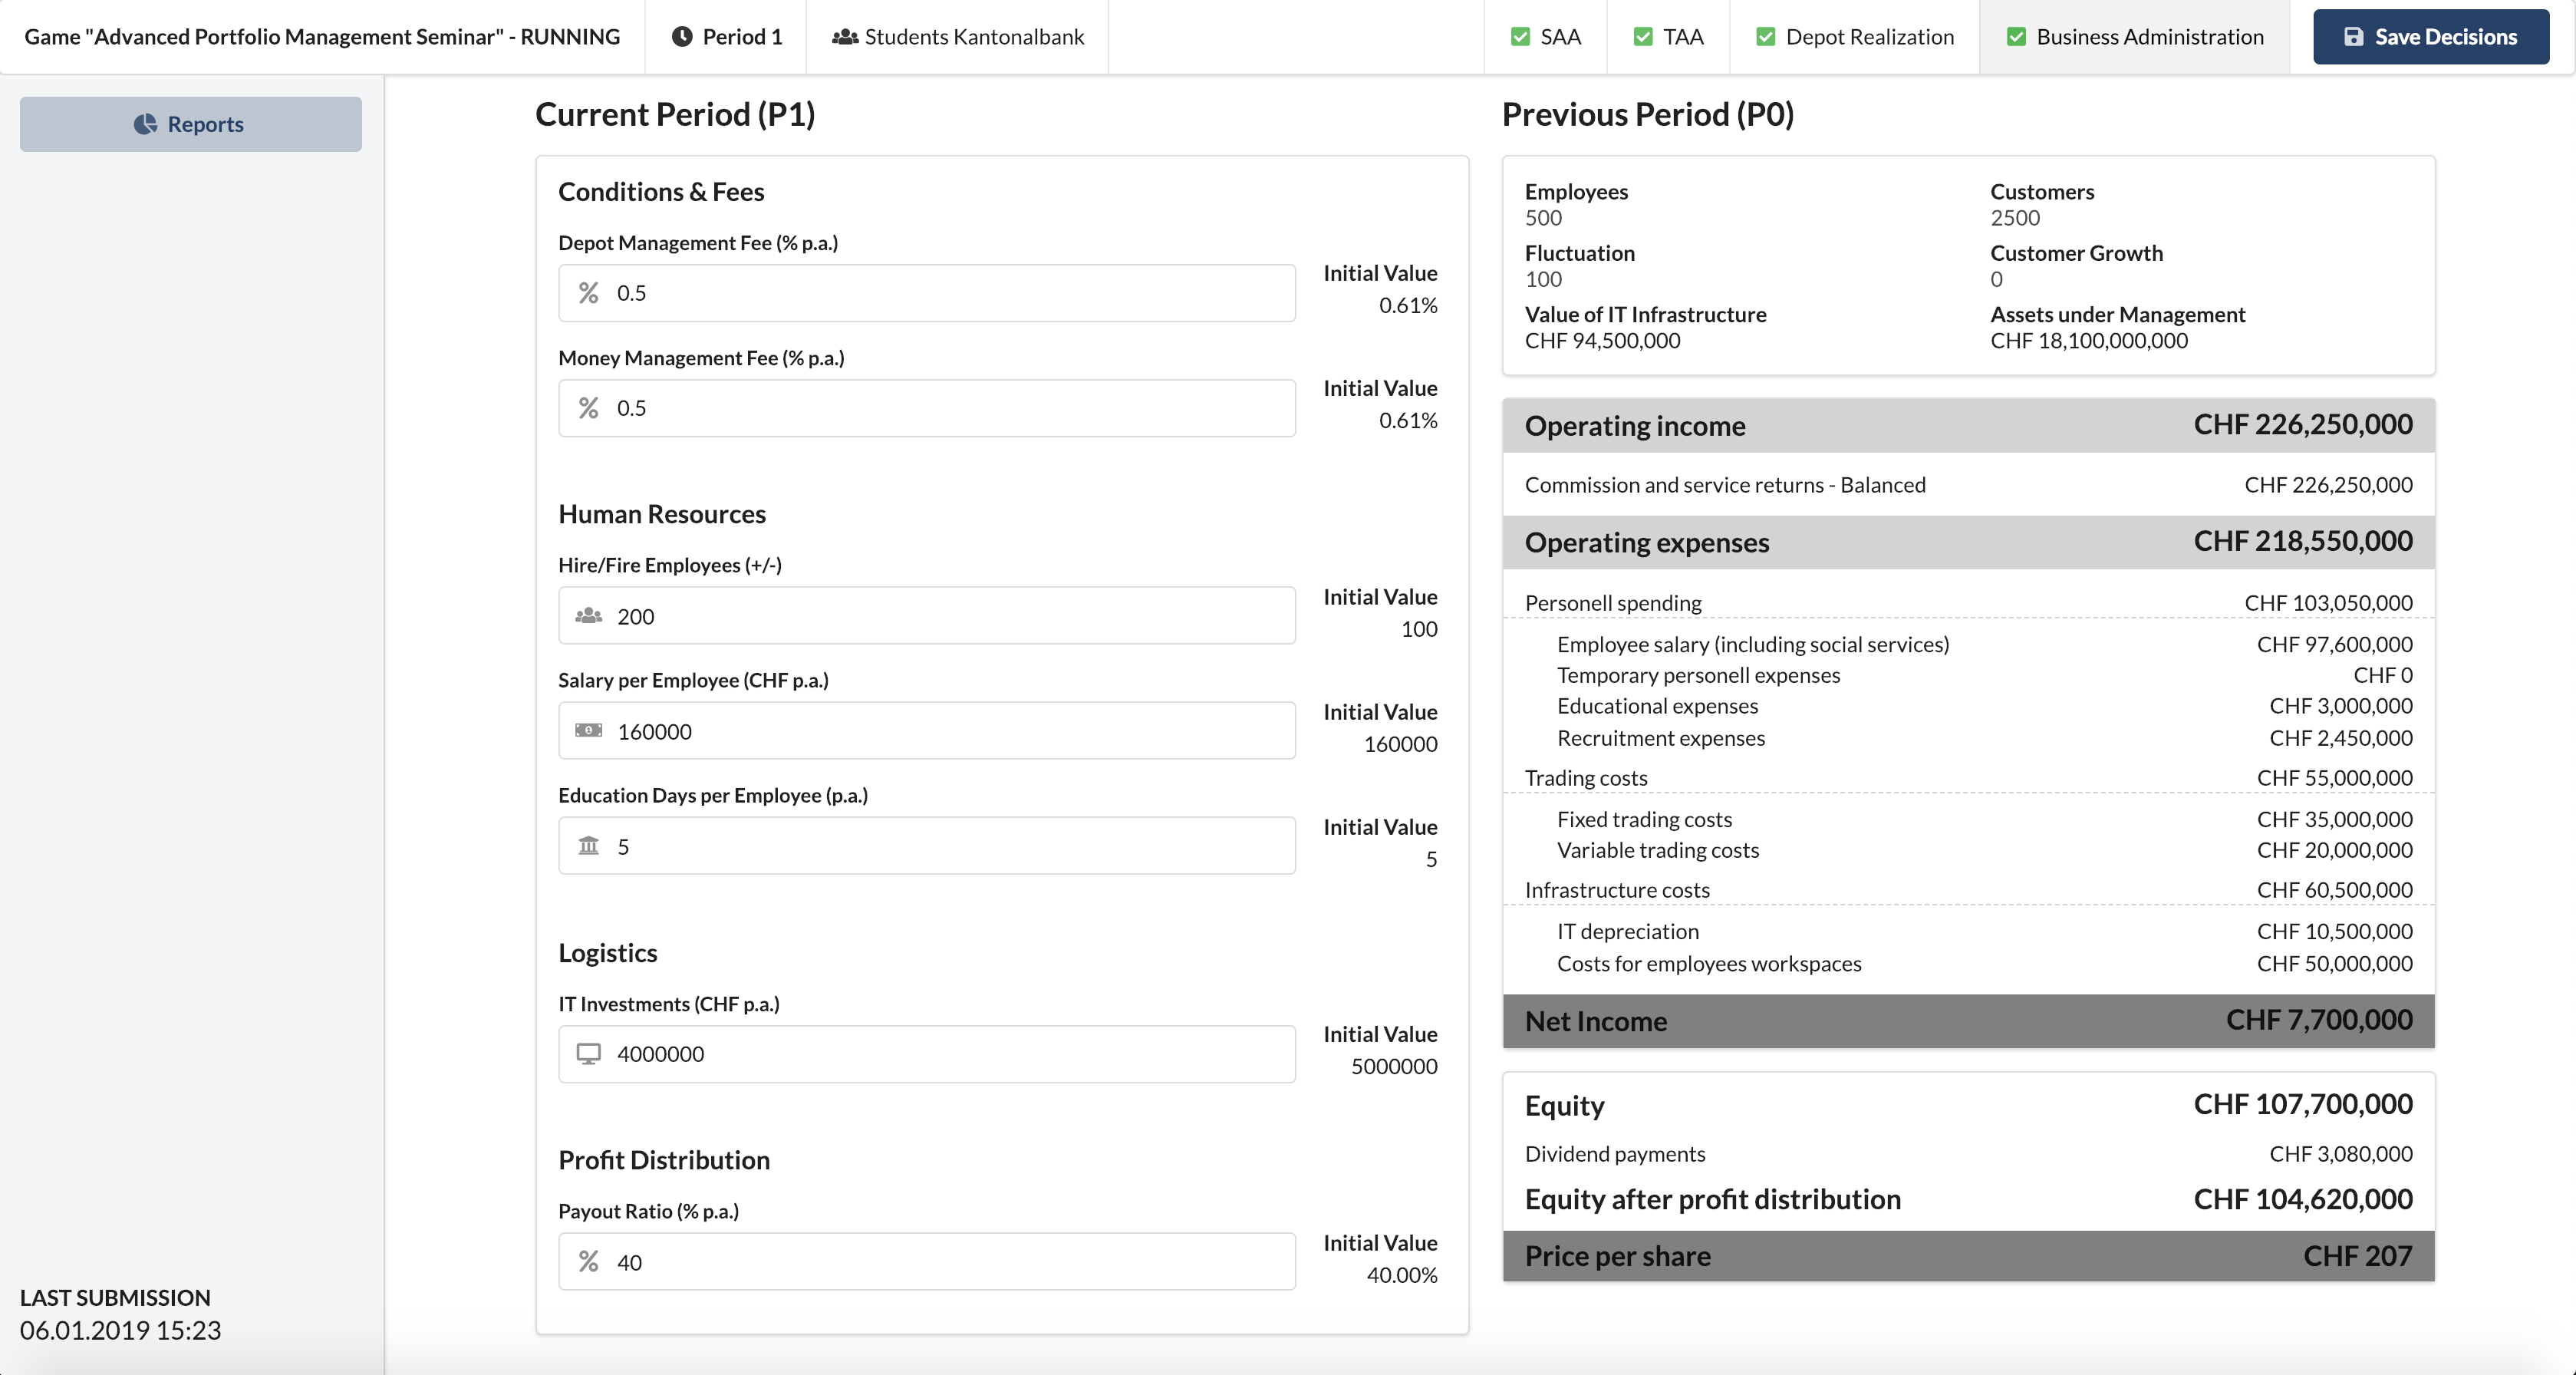
\includegraphics[scale=0.2]{img/application-overview/teams/06_business.png}
  \caption{Business Administration}
  \label{fig:business_admin}
\end{figure}


\subsection{Reports}
\label{subsec:reports}
Reports are available for both administrators of a game and teams. They explain the results of the different periods of each team and compare them to the results of the other teams. As there are many graphs available, they are structured into multiple tabs. The report section may be filtered by team and by periods to ensure that users can filter out the information that is relevant for them.

\subsubsection{Overview}
A short overview sets up the report page \Cref{fig:reports_overview}. A three-dimensional comparison between performance, total earnings, and assets under management should summarize up the investment profits of the teams, where each point represents a team at a specific period. The stock price development of the different teams shows the progress of the stock price over all periods. The best performing team concludes the last period of the game with the highest stock price. On the bottom of those graphs, there is a spider chart for each team describing all of the important indexes within a range of 0 to 10.
\begin{figure}[h!]
  \centering
  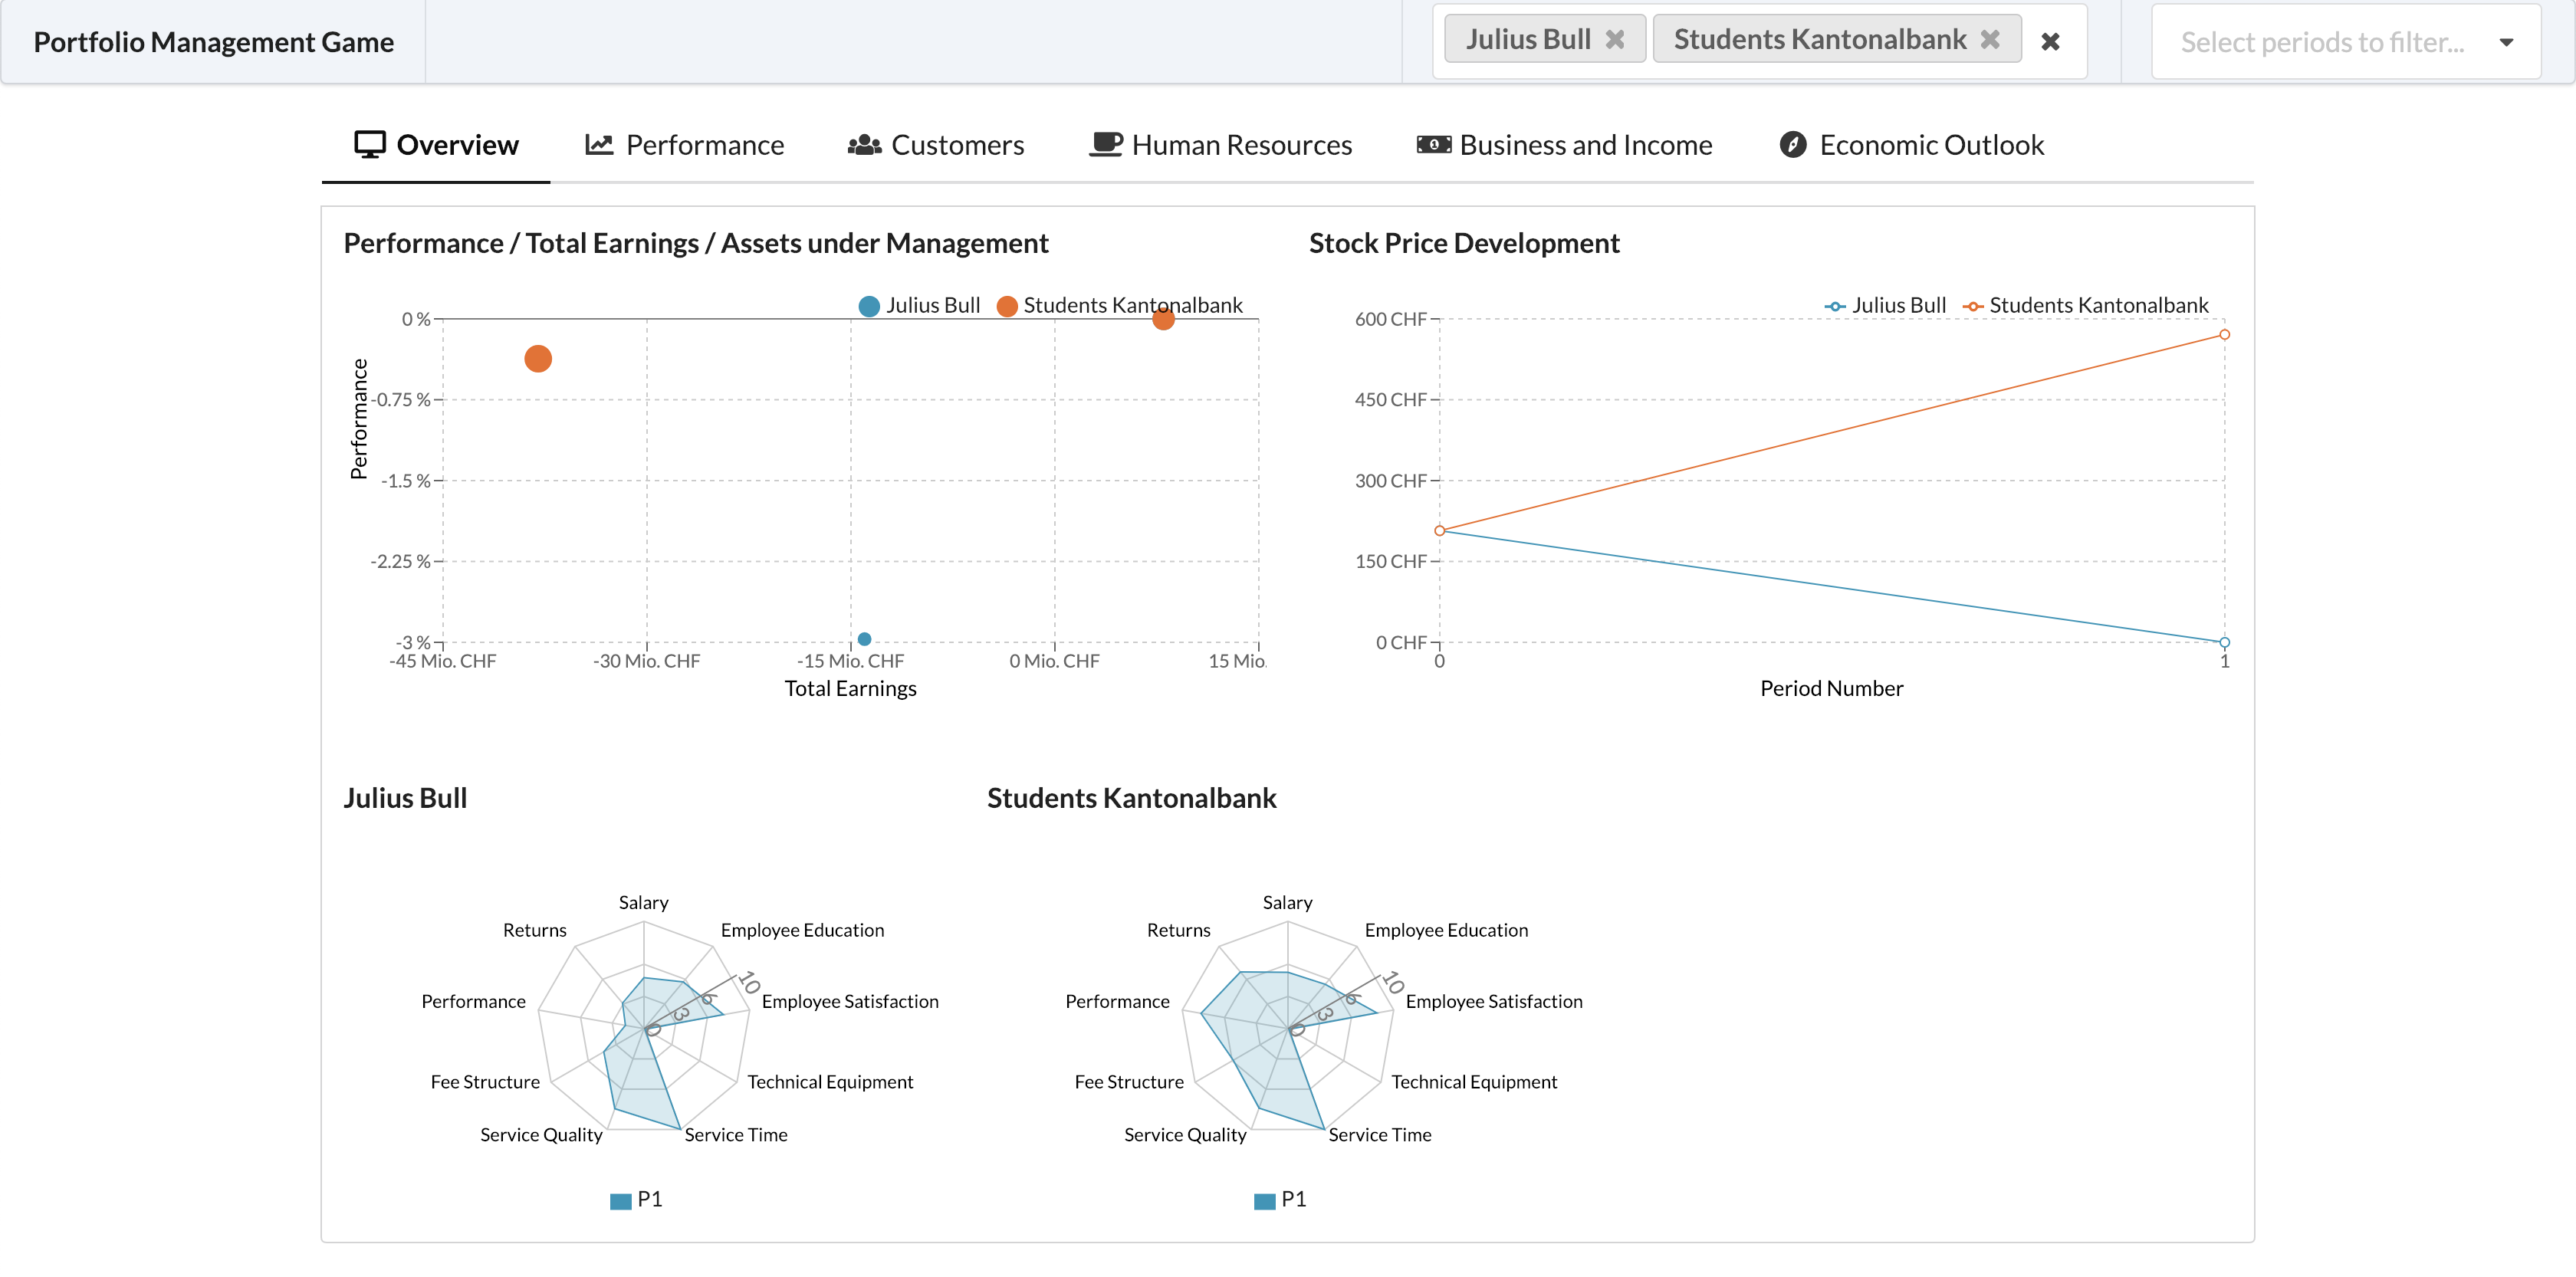
\includegraphics[scale=0.2]{img/application-overview/reports/01_overview.png}
  \caption{Reports - Overview}
  \label{fig:reports_overview}
\end{figure}

\subsubsection{Performance}
Multiple bar charts describe the performance of the teams for each customer type in each period. Exemplary measures include portfolio return, sharpe ratio, traynor ratio, jensen's alpha, and information ratio. An overview of those charts may be seen in \Cref{fig:reports_performance}
\begin{figure}[h!]
  \centering
  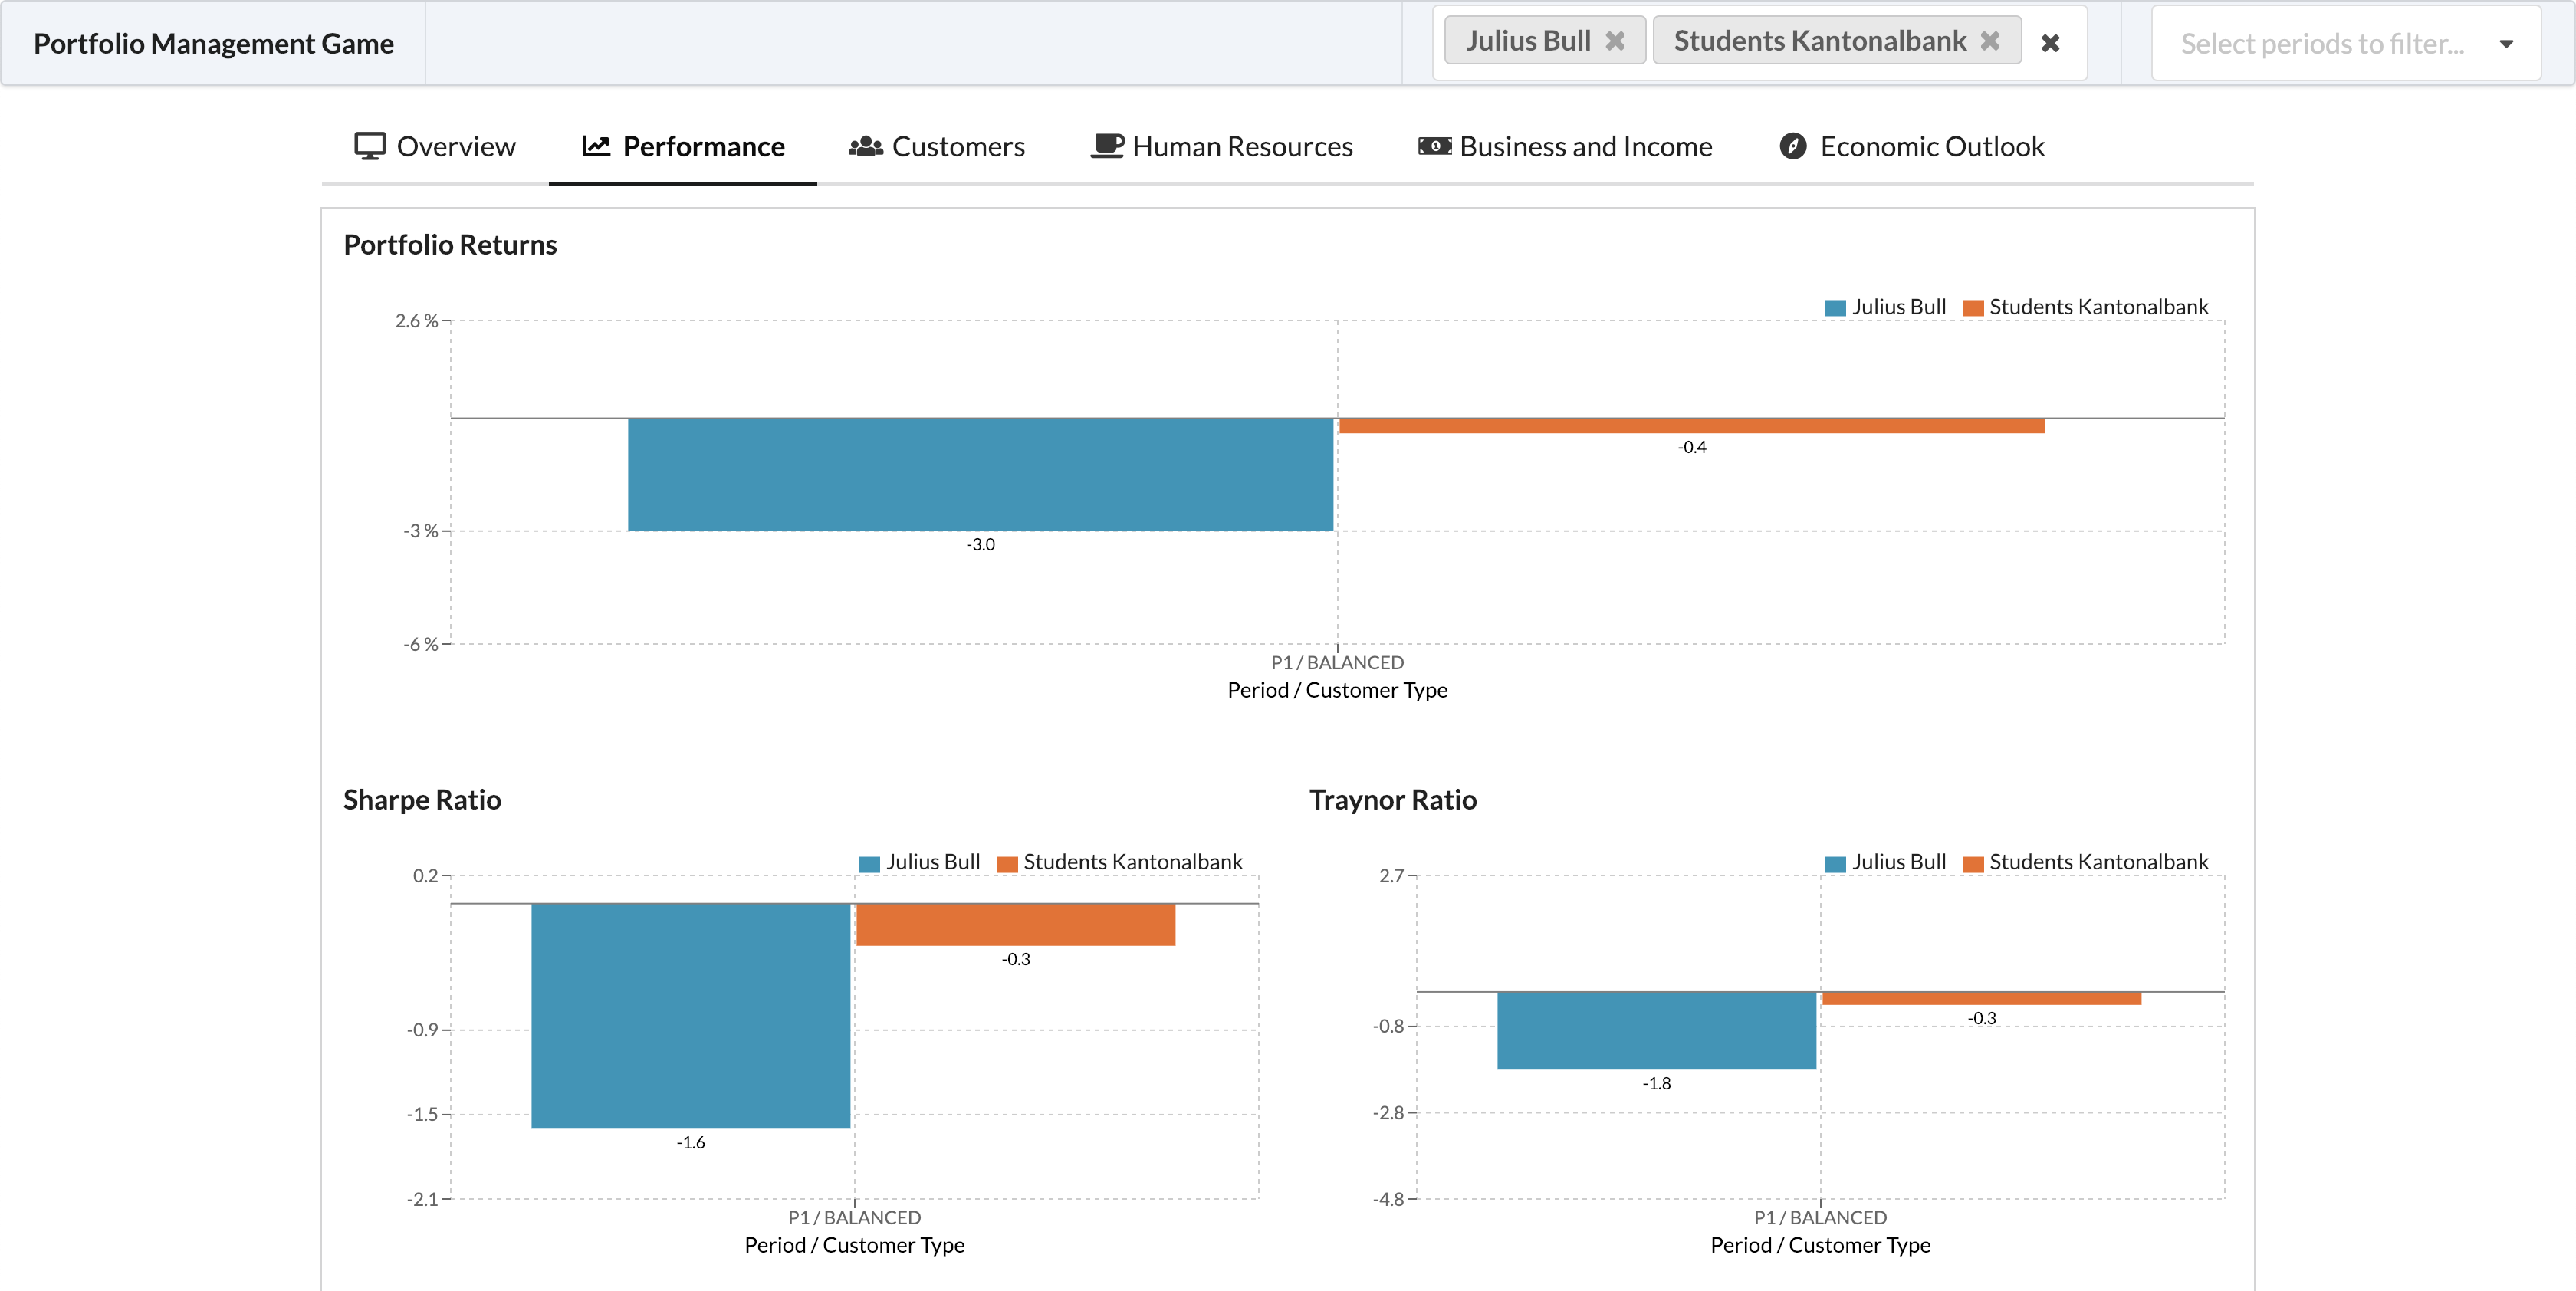
\includegraphics[scale=0.2]{img/application-overview/reports/02_performance.png}
  \caption{Reports - Performance}
  \label{fig:reports_performance}
\end{figure}

\subsubsection{Customers}
Similar to the performance tab, the customer section explains multiple key characteristics of customers for each team and period \Cref{fig:reports_customers}.
\begin{itemize}
  \setlength\itemsep{0.01em}
  \item Customer satisfaction index
  \item Number of Customers
  \item Customer growth
  \item Assets under management
  \item Net new money
  \item Relative TAA discrepancy (volume-weighted)
  \item Number of SAA violations
\end{itemize}
\begin{figure}[h!]
  \centering
  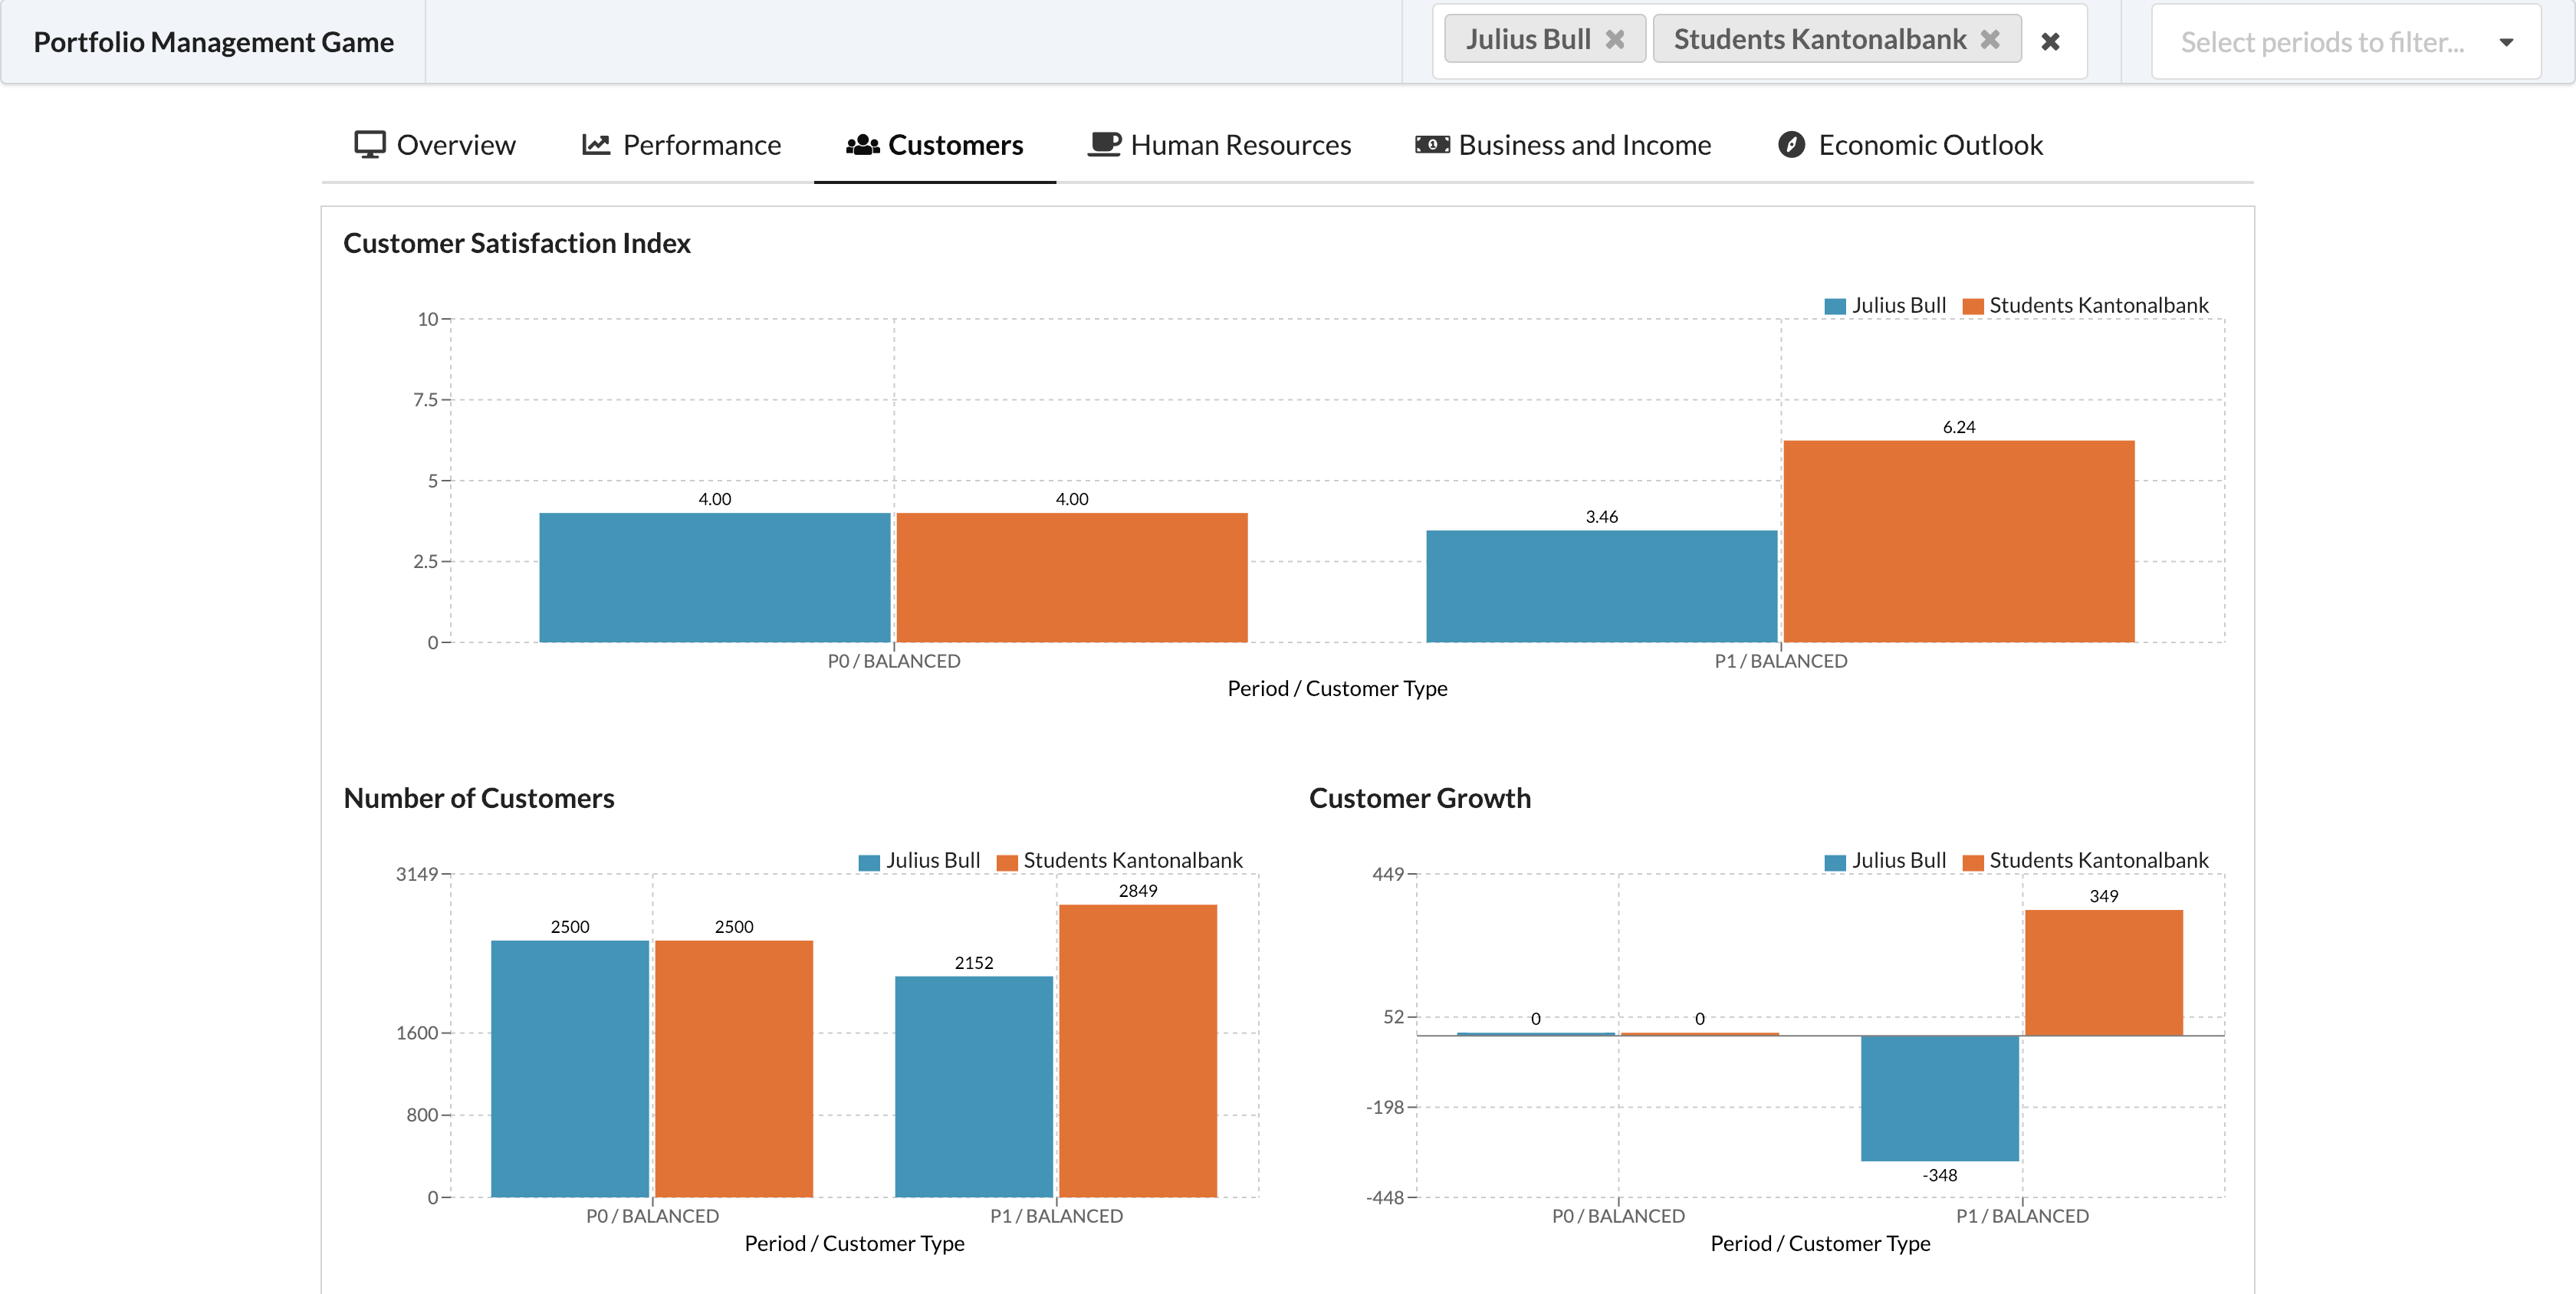
\includegraphics[scale=0.2]{img/application-overview/reports/03_customers.png}
  \caption{Reports - Customers}
  \label{fig:reports_customers}
\end{figure}

\subsubsection{Human Resources}
Information about human resources (HR) is currently displayed using four bar charts: employee satisfaction index, number of employees, salary index, and education index. \Cref{fig:reports_hr} shows an exemplary scenario.
\begin{figure}[h!]
  \centering
  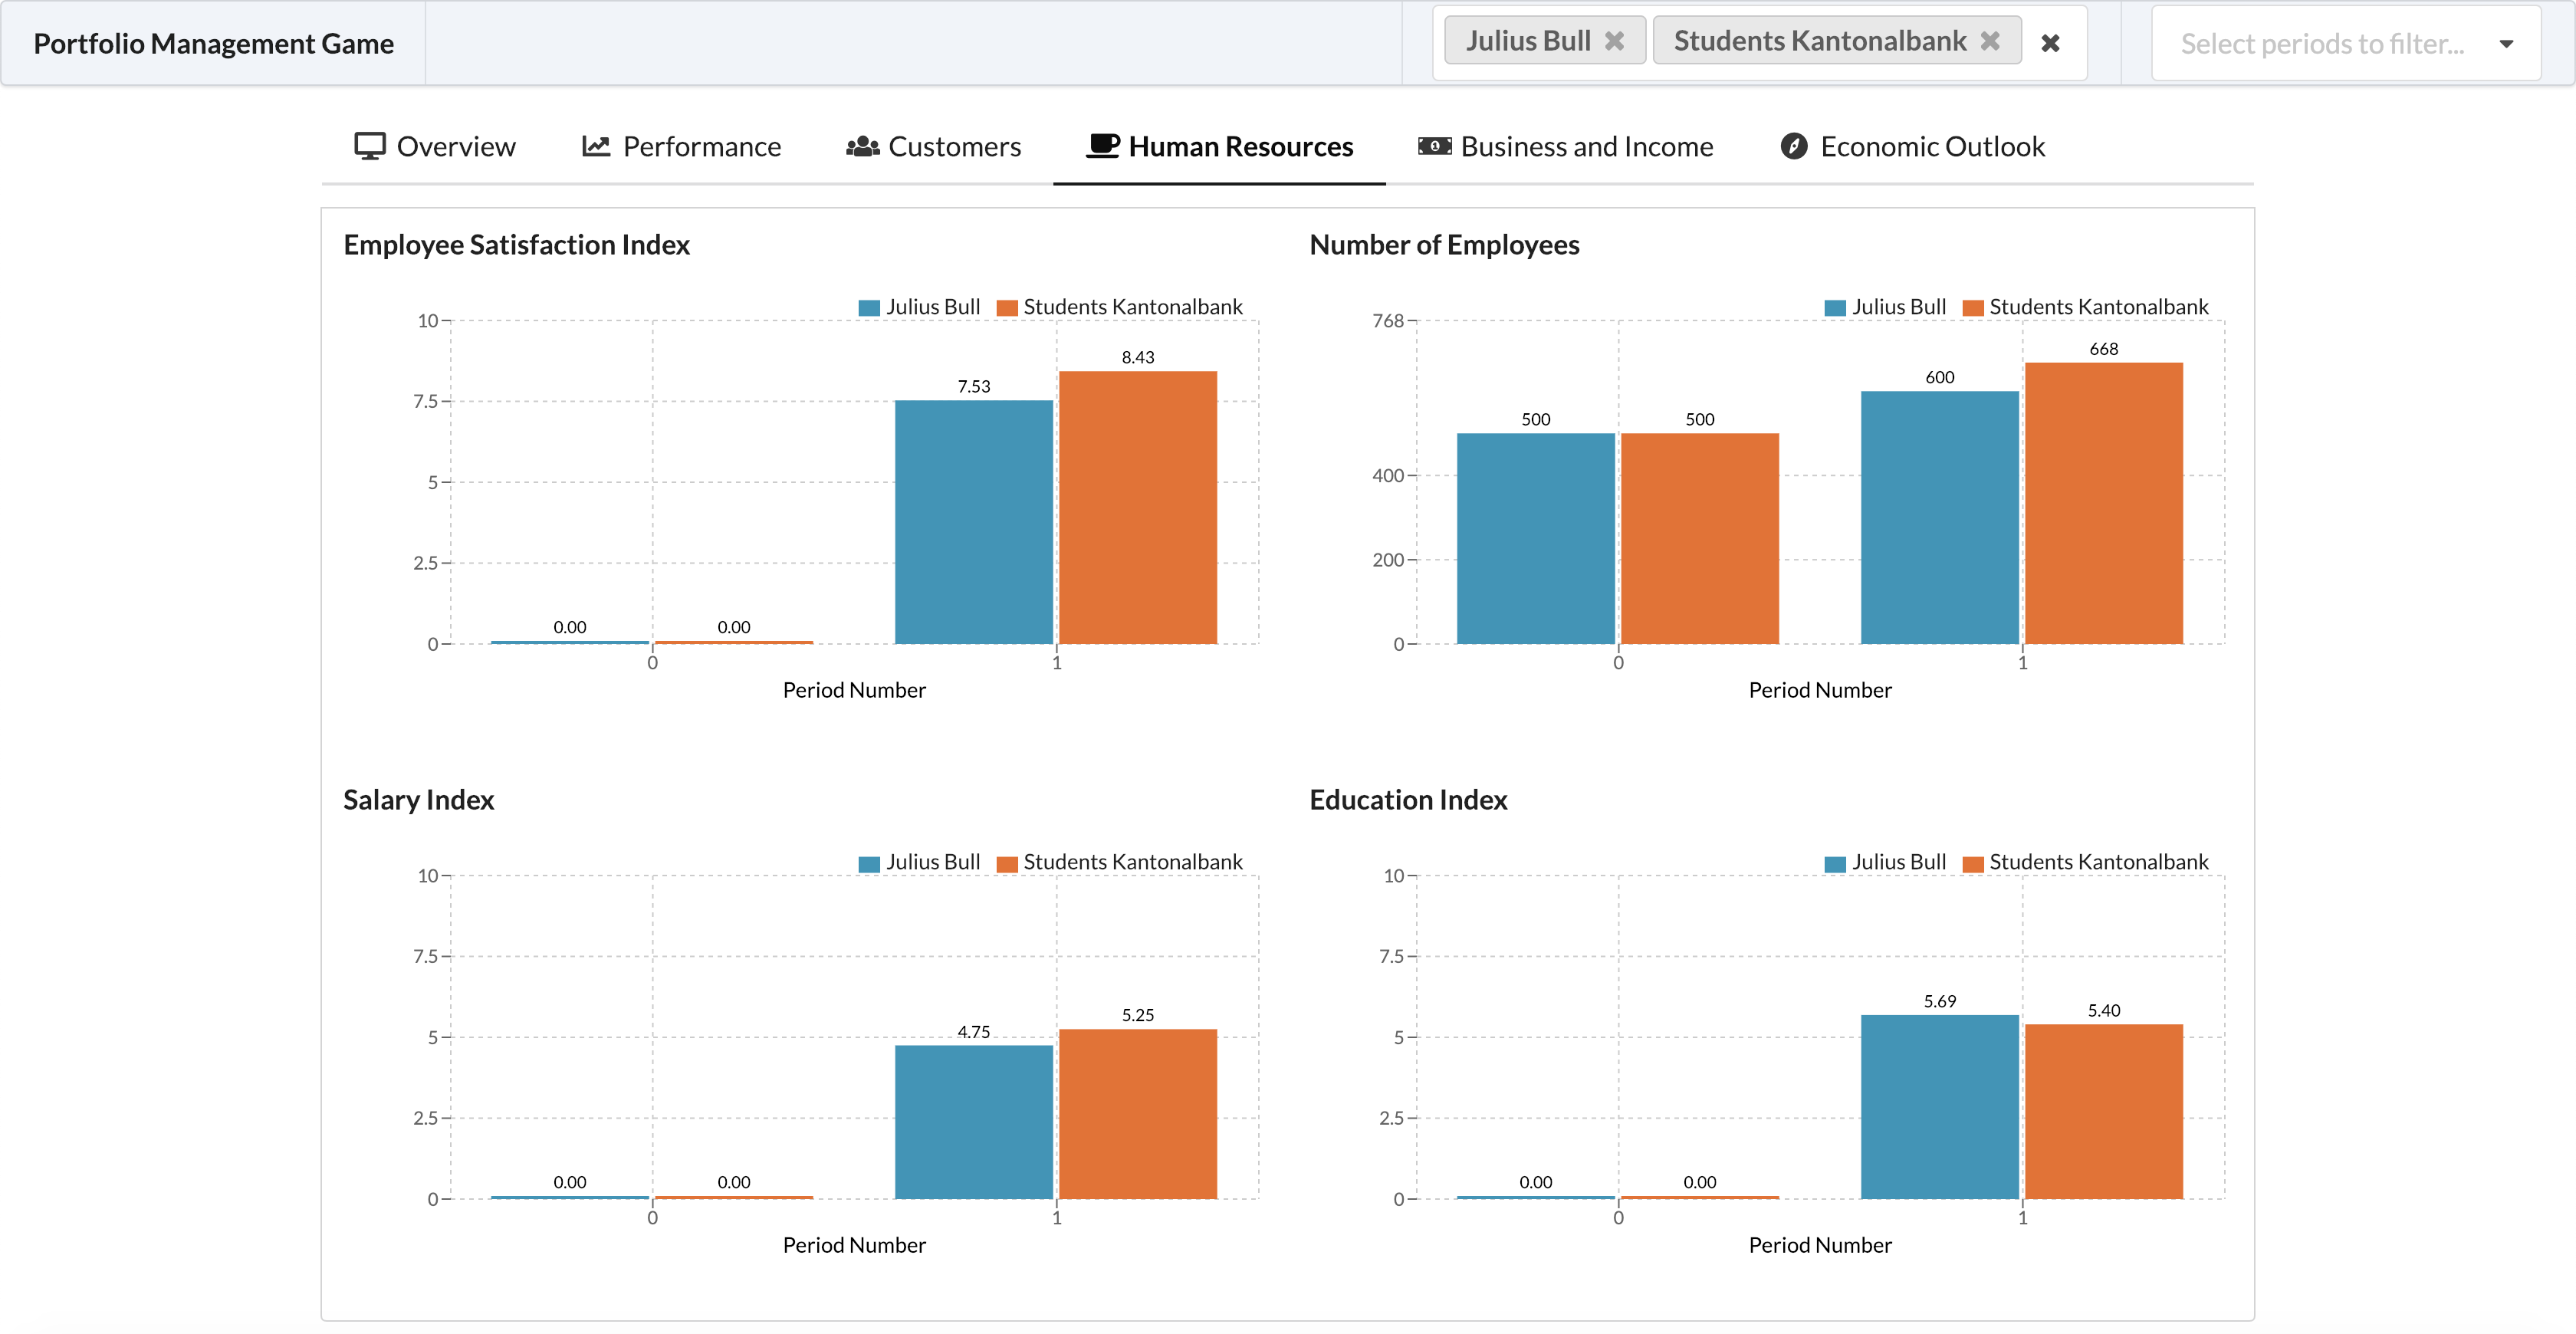
\includegraphics[scale=0.2]{img/application-overview/reports/04_hr.png}
  \caption{Reports - Human Resources}
  \label{fig:reports_hr}
\end{figure}

\subsubsection{Business and Income}
Starting with four bar charts (\Cref{fig:reports_business_income}) this tab explains the results of the teams' business decisions, such as operating income, operating expenses, cost income ratio, and net income. In \Cref{fig:reports_balance_sheet_comparison} different teams in different periods can be compared by their balance sheet. The users can either compare previous periods with upcoming of their own balance sheet or compare their own result to other teams in the same period.
\begin{figure}[h!]
  \centering
  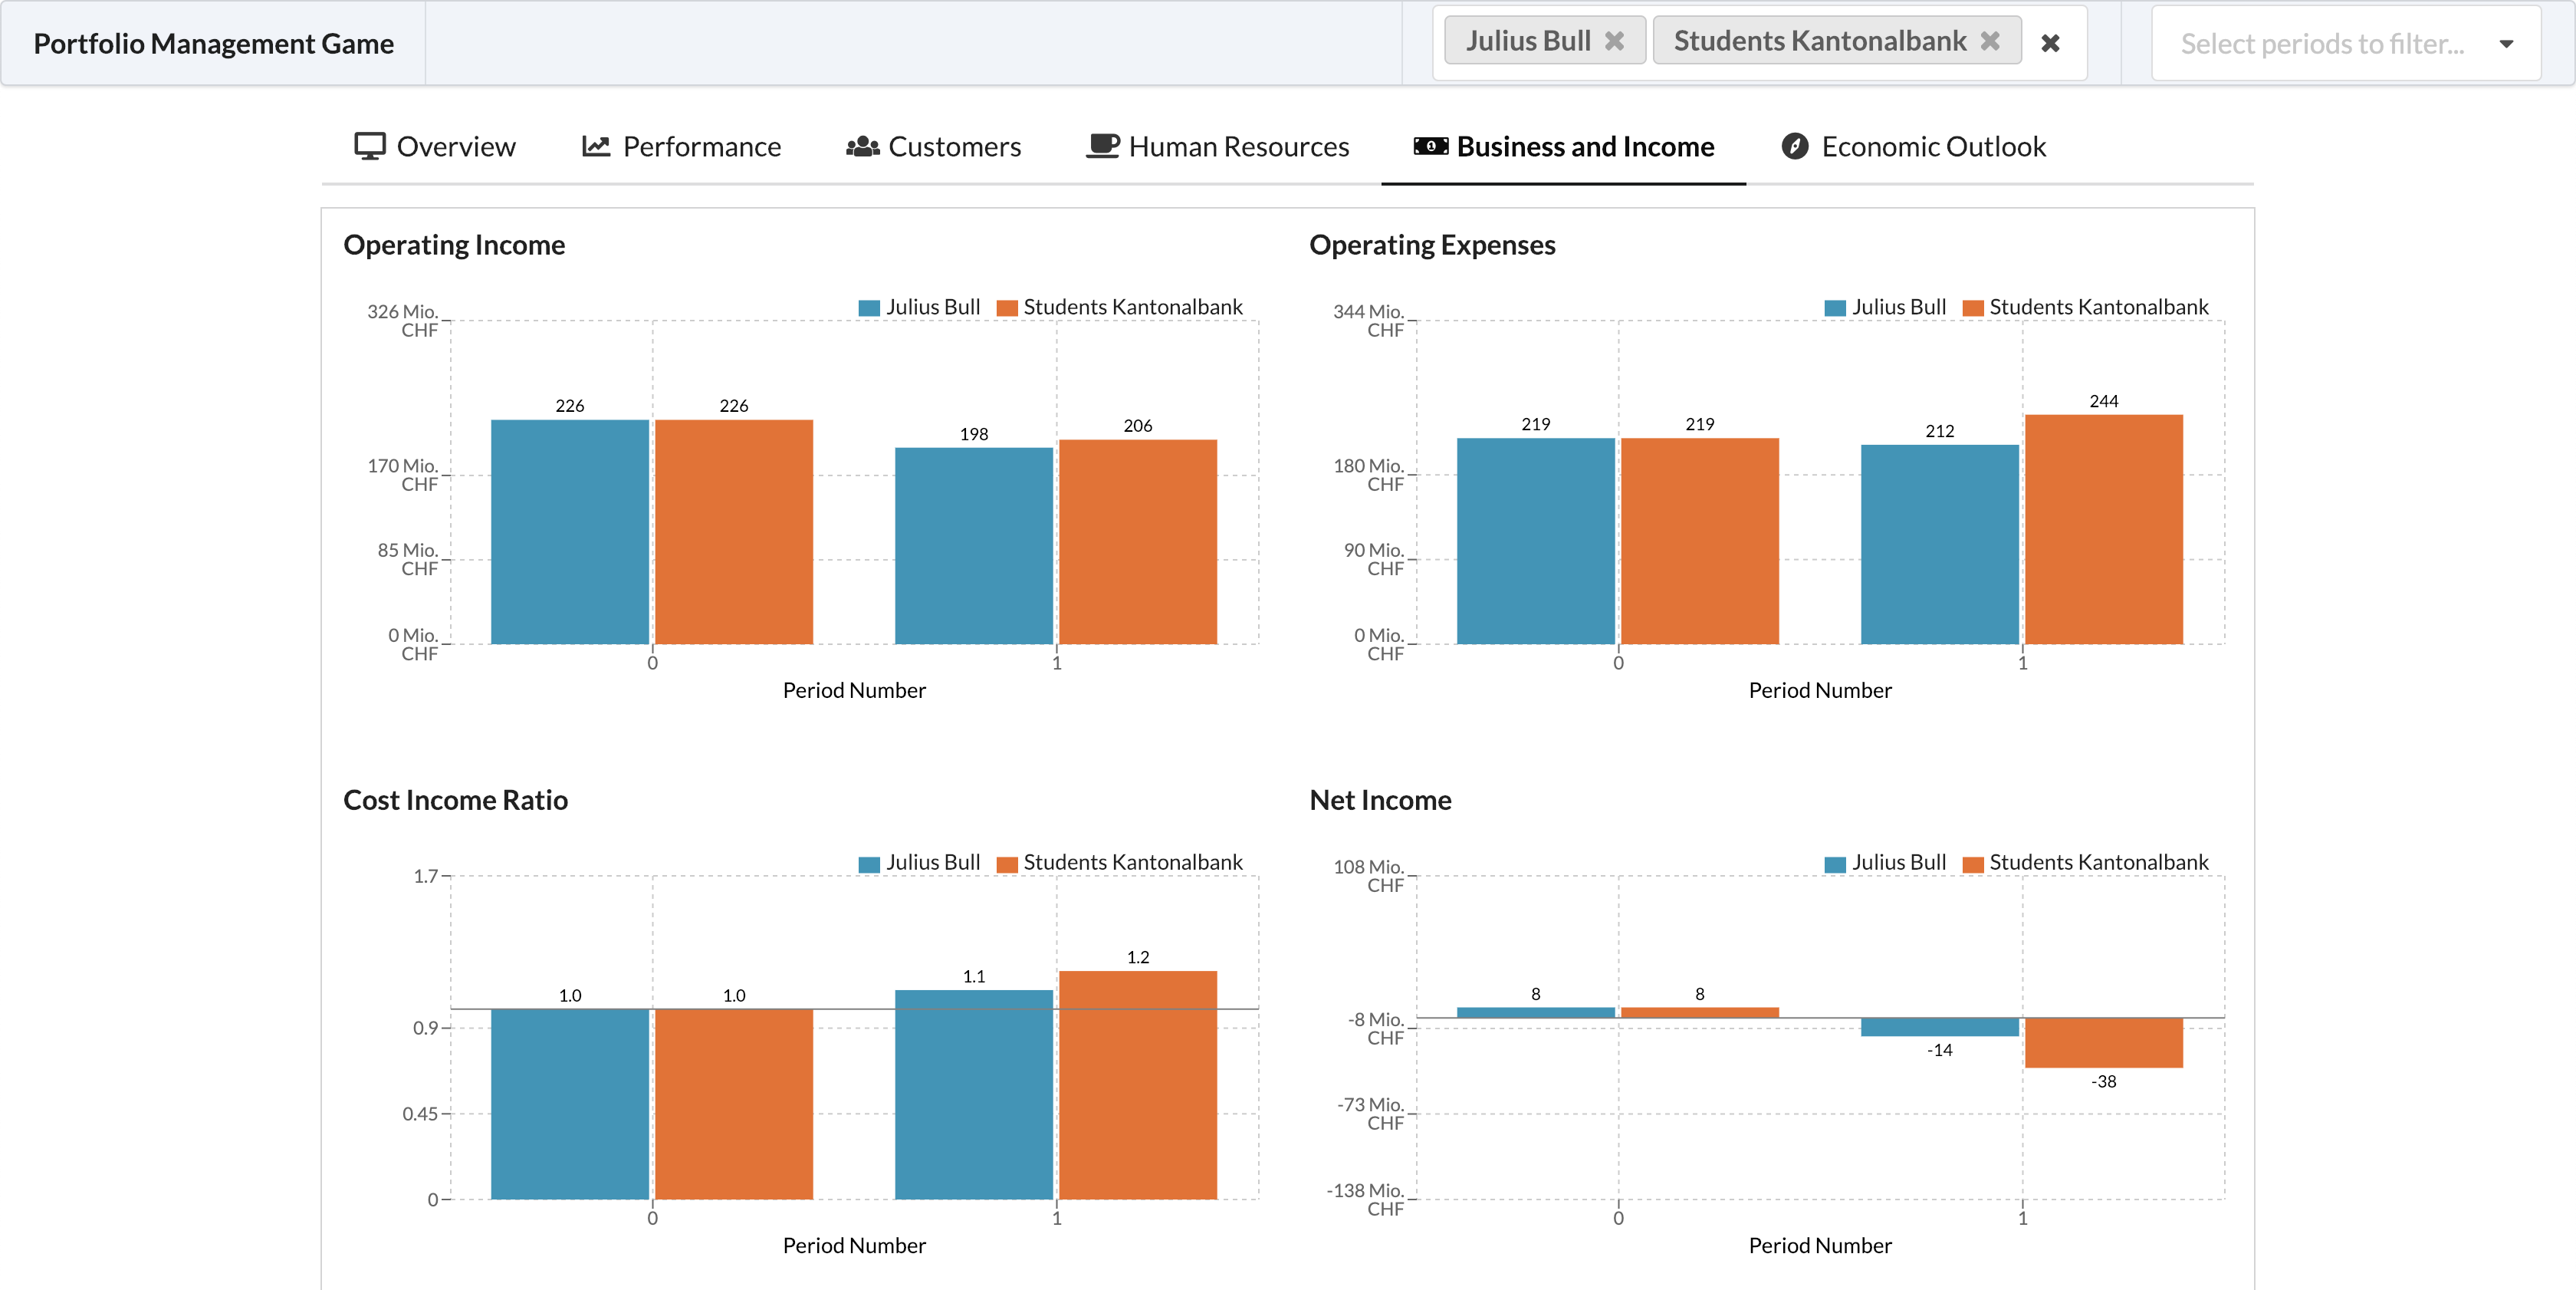
\includegraphics[scale=0.2]{img/application-overview/reports/05_business_income.png}
  \caption{Reports - Business and Income}
  \label{fig:reports_business_income}
\end{figure}
\begin{figure}[h!]
  \centering
  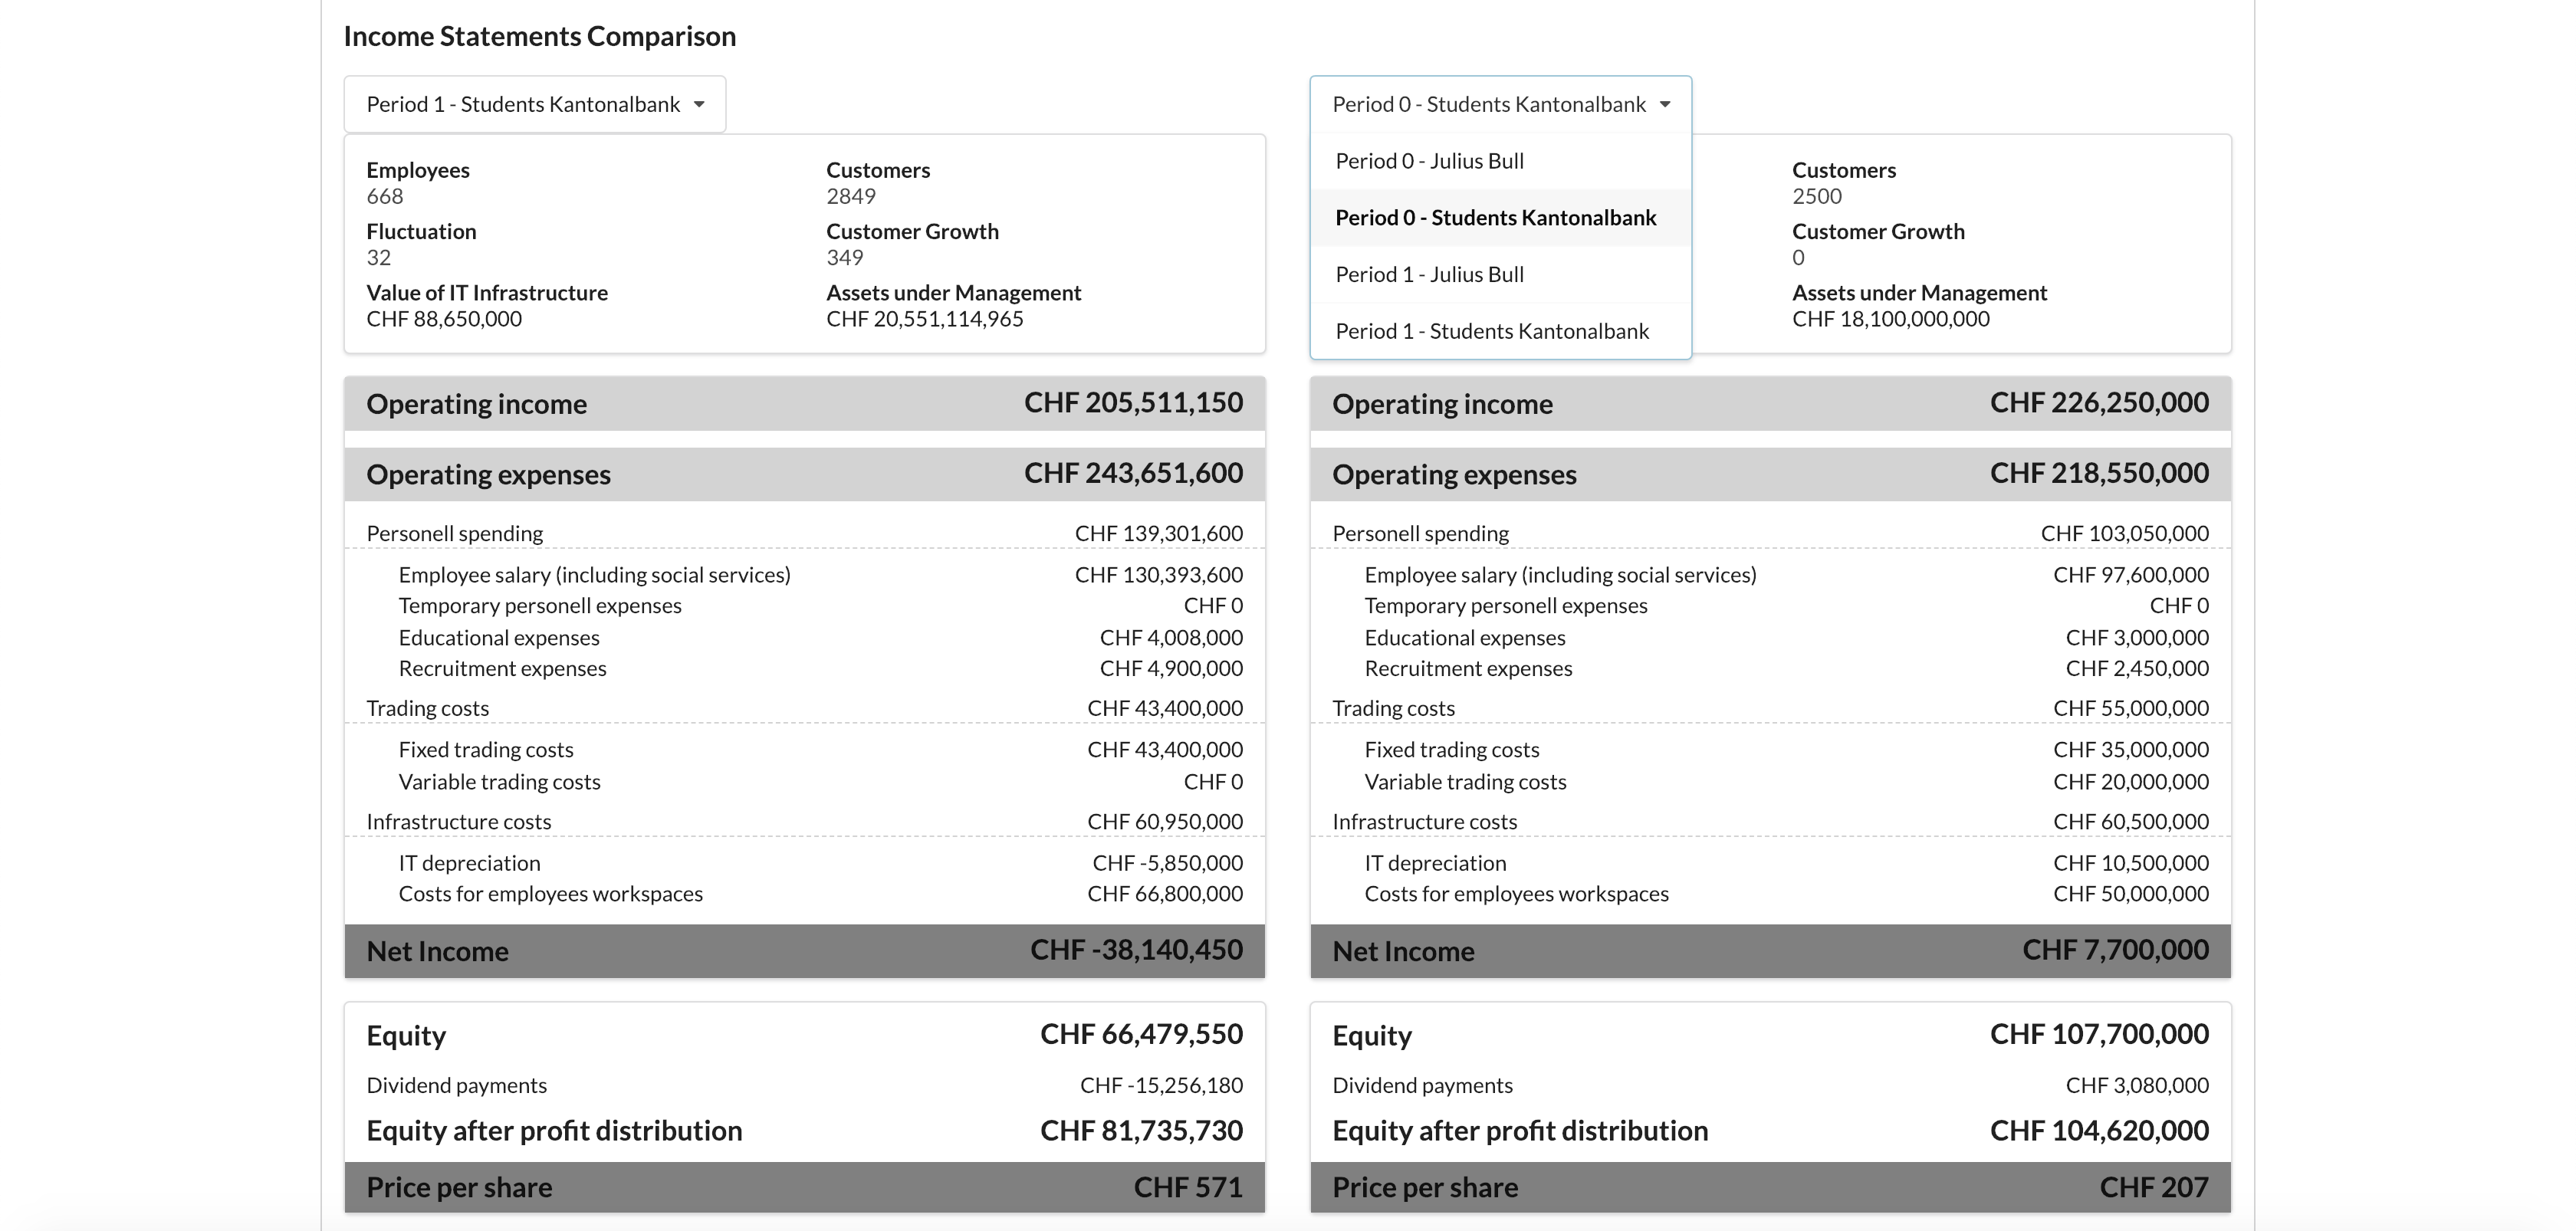
\includegraphics[scale=0.2]{img/application-overview/reports/05_business_income_balance_sheet_comparison.png}
  \caption{Reports - Balance Sheet Comparison}
  \label{fig:reports_balance_sheet_comparison}
\end{figure}


\subsubsection{Economic Outlook}
The economic outlook is the only tab that is already accessible starting from period 2, as all other graphs or tabs are only calculated once teams have made their first decisions in period one (\Cref{fig:reports_outlook}).
\begin{figure}[h!]
  \centering
  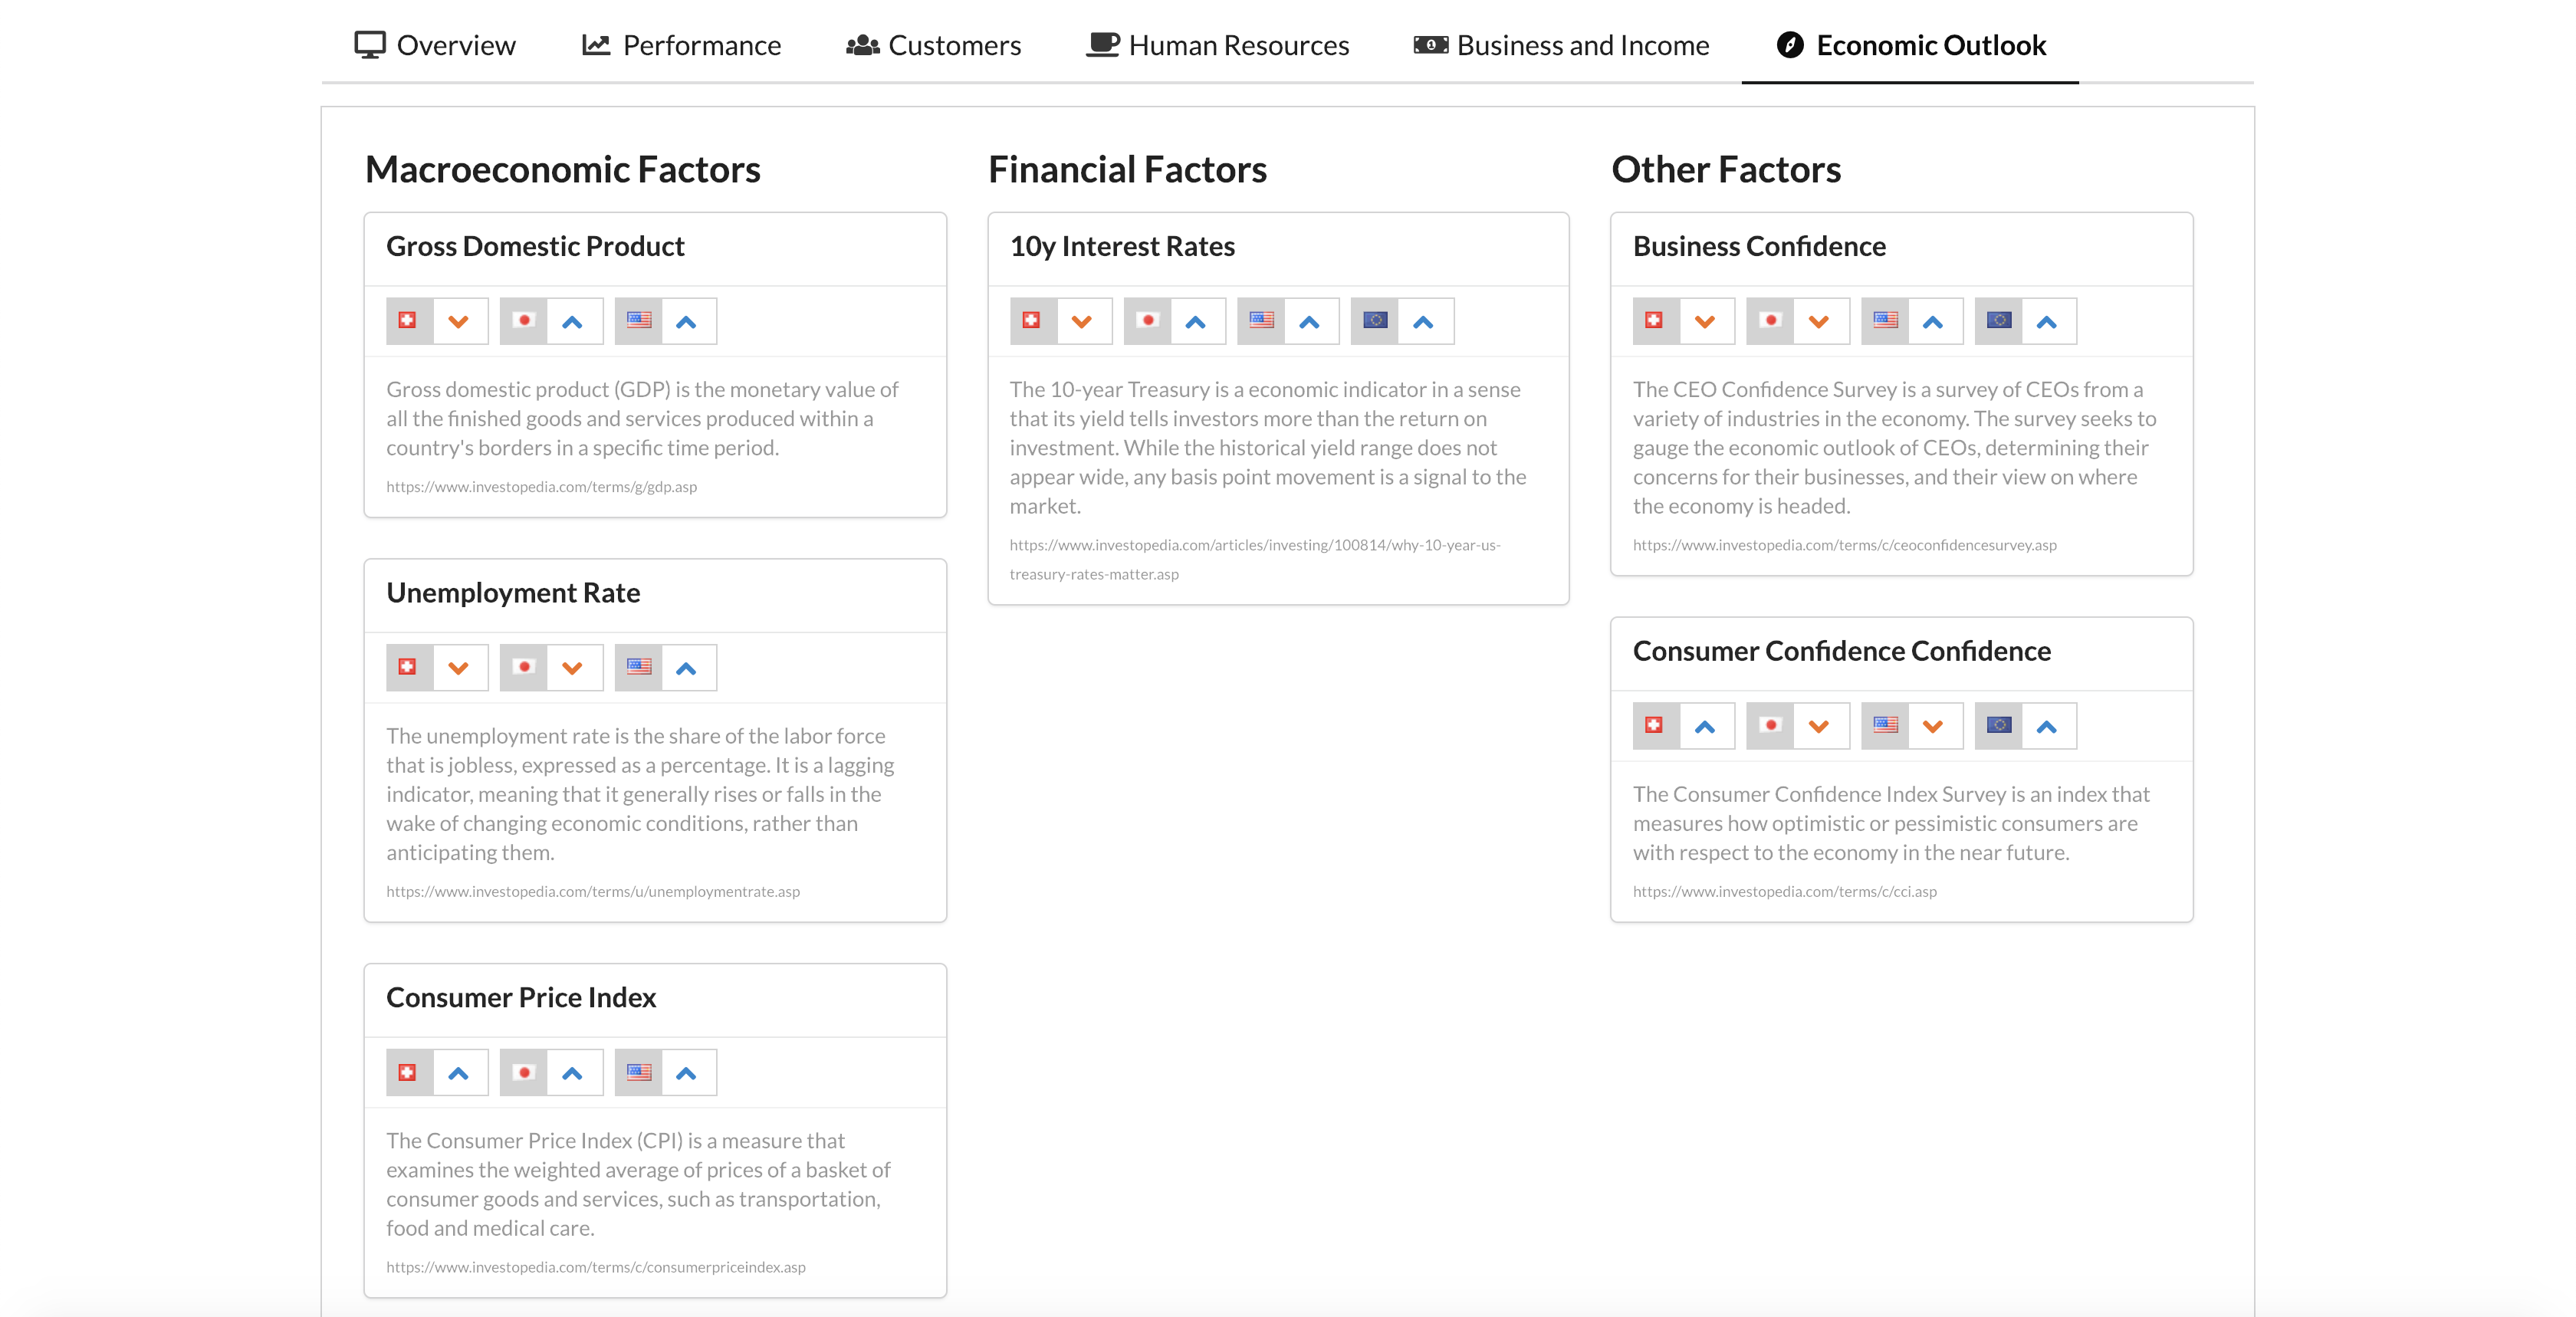
\includegraphics[scale=0.2]{img/application-overview/reports/06_economic_outlook.png}
  \caption{Reports - Economic outlook}
  \label{fig:reports_outlook}
\end{figure}
